\documentclass[11pt]{gsasthesis} % 10,11 and 12pt fonts allowed

%%%%%%%%%%%%%%%% PACKAGES YOU PROBABLY WANT %%%%%%%%%%%%%%%%
% Include packages you want. The gsasthesis style file already includes
% packages "setspace" and "tocbibind".

\usepackage{etex} % extend the number of registers

% GSAS: "all margins should be at least 1 inch."
\usepackage[margin={1.2in}]{geometry}
% If you want asymmetric margins for two-sided documents, use the "twoside"
% option, as in
% \usepackage[top=1in,bottom=1.5in,left=1in,right=1.5in,twoside]{geometry} The
% left and right options become inner and outer margins The default horizontal
% latex margin ratio is 2:3. The default vertical top:bottom margin ratio is 2:3
% also. You can also set it directly by passing the hmarginratio option to the
% geometry package, as in
% \usepackage[top=1in,left=1in,vmarginratio=2:3,hmarginratio=2:5,twoside]{geometry}

% Appendix package. Not necessary, but it does make managing appendices easier
\usepackage[titletoc]{appendix}

%%%%%%%%%%%%%%%% PACKAGES MAY WANT %%%%%%%%%%%%%%%%

% sideways tables and figures
\usepackage{rotating}

% tables that spill over multiple pages
\usepackage{longtable}

% references
\usepackage{natbib}

% fonts that are nicer than defaults
% \usepackage[sc]{mathpazo}
% \usepackage{courier}

% Use 8-bit encoding that has 256 glyphs, pretty please
\usepackage[utf8]{inputenc}
\usepackage[T1]{fontenc}

% babel is required for blindtext, which generates random text
\usepackage[english]{babel}
\usepackage{blindtext}

% math support
\usepackage{amsmath}
\usepackage{amssymb}
\usepackage{gensymb}

% Slightly tweak font spacing for aesthetics
\usepackage{microtype}
\usepackage{enumitem}

\usepackage{caption}    % Helps with subcaptions
\usepackage{subcaption} % For individual subfigures

% AAS macros
\usepackage{aas_macros}
\usepackage{hyperref}
\newcommand{\dodoi}[1]{\href{https://doi.org/#1}{doi:#1}}

\usepackage{color}
\usepackage{graphicx}

\usepackage{deluxetable}
% \usepackage{changepage,parskip}
\usepackage{changepage}

% \usepackage{bibentry}
% \nobibliography*

% You need the footmisc package with the stable option if you want to have
% footnotes inside section titles, for example to say that a particular chapter
% has been co-authored with someone. The multiple option ensures that there is a
% comma between two consecutive footnotes
\usepackage[stable,multiple]{footmisc}

\newcommand{\Msun}{\ensuremath{M_{\odot}}}
\newcommand{\Gyr}{\ensuremath{\textrm{Gyr}}}
\newcommand{\Myr}{\ensuremath{\textrm{Myr}}}
\newcommand{\yr}{\ensuremath{\textrm{yr}}}
\newcommand{\kpc}{\ensuremath{\textrm{kpc}}}
\newcommand{\ckpc}{\ensuremath{\textrm{ckpc}}}
\newcommand{\pc}{\ensuremath{\textrm{pc}}}
\newcommand{\kms}{\ensuremath{\textrm{km}/\textrm{s}}}
\newcommand{\tocite}{\textcolor{blue}{cite}}
\newcommand{\FeH}{\ensuremath{[\textrm{Fe}/\textrm{H}]}}
\newcommand{\MgFe}{\ensuremath{[\textrm{Mg}/\textrm{Fe}]}}
\newcommand{\OFe}{\ensuremath{[\textrm{O}/\textrm{Fe}]}}
\newcommand{\alphaFe}{\ensuremath{[\alpha/\textrm{Fe}]}}
\newcommand{\tform}{\ensuremath{t_{\textrm{form}}}}
\newcommand{\dex}{\ensuremath{\textrm{dex}}}
\newcommand{\Msunyr}{\ensuremath{\Msun/\textrm{yr}}}
\newcommand{\Msunyrdex}{\ensuremath{\Msun/\textrm{yr}/\textrm{dex}}}
\newcommand{\Atmax}{\ensuremath{A_{2,\textrm{max}}}}

\newcommand{\rhalf}{\ensuremath{r_{\star,\textrm{half}}}}
\newcommand{\SFR}{\ensuremath{\textrm{SFR}}}

\newcommand{\RCR}{\ensuremath{R_{\textrm{CR}}}}
\newcommand{\Rot}{\ensuremath{\mathcal{R}}}
\newcommand{\Vc}{\ensuremath{V_{\textrm{c}} }}
\newcommand{\PS}{\ensuremath{\Omega_{\textrm{p}}}}
\newcommand{\Rb}{\ensuremath{R_{\textrm{b}}}}

\newcommand{\Nbody}{$N$-body}
\newcommand{\AREPO}{\textsc{AREPO}}
\newcommand{\SMUGGLE}{SMUGGLE}

\newcommand{\doi}[2]{\href{http://dx.doi.org/#1}{{#2}}}
\newcommand{\arxiv}[3]{\href{http://arxiv.org/abs/#1}{{#2}\textcolor{black}{, \textit{Submitted to #3}}\ \textcolor{grey}{\texttt{arXiv:#1}}}}
\newcommand{\arxivaccept}[3]{\href{http://arxiv.org/abs/#1}{{#2}\textcolor{black}{, \textit{Accepted in #3}}\ \textcolor{black}{\texttt{arXiv:#1}}}}

% Nicer captions
\RequirePackage[font=small,format=plain,labelfont=bf,textfont=it]{caption}
\addtolength{\abovecaptionskip}{1ex}
\addtolength{\belowcaptionskip}{1ex}

%%%%%%%%%%%%%%%% COMPULSORY FIELDS %%%%%%%%%%%%%%%%

\title{Rising from the Ashes\\How the Milky Way Got Its Scars} % needs to match title on DAC
\author{Angus William Beane} % full name as it appears on your GSAS record, needs
                          % to match name on DAC
\degreename{Doctor of Philosophy}
\degreefield{Astronomy \& Astrophysics} % Official name of subject as listed in GSAS
                                % handbook
\department{The Department of Astronomy} % official name of department
\degreemonth{March} % Month of Defense (i.e. month when DAC was signed)
\degreeyear{2025} % Year the DAC was signed
\principaladvisor{Professor Lars Hernquist}

% Optionally, you can add a second advisor, but you can't have three
% \secondadvisor{Professor George Secondary}



\begin{document}

%%%%%%%%%%%%%%%% FRONTMATTER %%%%%%%%%%%%%%%%

\pagenumbering{roman} % GSAS wants roman page numbers for frontmatter

% the following four pages are required in that order. The first two pages are
% not allowed to have page numbers, this is taken care of in the class file.
\thesistitlepage
\copyrightpage
\begin{abstract}
  Understanding ancient events in the Milky Way's history is essential for building a consistent picture of galaxy formation and evolution, bridging stellar and chemical evolution models with the extragalactic population. Our galaxy experienced three simultaneous, transformative events $8\,\Gyr$ ago: our last major merger, the formation of a bar, and a transition chemical enrichment leading to an $\alpha$-element bimodality. The history of these events is encoded in the present-day observable properties of stars: dynamics (positions and velocities), chemical compositions, and ages. In this thesis, we will make use of numerical simulations tailored to understanding how these historical processes of the Milky Way led to its present-day properties. First, we will propose a solution to the mystery of why the bar rotates rapidly when it is old enough to have slowed down by now. Second, we will propose that our last major merger led to the emergence of the $\alpha$-bimodality via a metallicity-dependent halt in star formation. Finally, we will demonstrate that the formation of the bar might have triggered the formation of the bimodality through the same mechanism. This work demonstrates the rich understandings that can be gleaned from idealized simulations specifically tailored to the Milky Way.
\end{abstract}

% Center headings for table of contents, LOT, and LOF and make them smaller so
% that "Abstract", "Acknowledgments" and "Contents" all look alike. Comment out
% if you want the default. If you want more control, use the "tocloft" package.
\renewcommand{\contentsname}{\protect\centering\protect\Large Table of Contents}
\renewcommand{\listtablename}{\protect\centering\protect\Large List of Tables}
\renewcommand{\listfigurename}{\protect\centering\protect\Large List of Figures}

\tableofcontents % Table of contents

% The rest of the front matter: Lists of tables, figures, dedication and
% acknowledment is optional. Comment out whatever you don't like
% \listoftables
% \listoffigures
% !TEX root = ms.tex

\begin{acknowledgments}
  To be finalized

  % In many other programs with many other advisors, mentors, and peers, I might not have finished my PhD. I have been extraordinarily lucky to have stumbled from one mentor exemplifying dedication, kindness, selflessness, and the height of competency to another, providing me with an ideal container to start my academic career.

  % In order to understand the Milky Way one must first exist in it, and for that I have to thank my parents, Anne and Tim Beane. No matter who I become or what I choose to do, they have repeatedly ensured that I understand I have their unconditional love and support. They dedicated nearly three decades of their lives to raising myself and my siblings. Enumerating all of their sacrifices would lead the university to consider implementing a strict page limit on acknowledgments. 

  % As the youngest, my siblings have literally always been there for me. 

  % I was encouraged by numerous teachers to pursue all my interests, including not just in physics. The math and science specialty center gave me an environment to see what science is at an early stage. I learned a lot from my teachers, including Mrs. Cope, Mrs. Delano, Mr. Fetsko, Mr. Gallo, and Mrs. Watson.

  % However, no one was as impactful during my high school years than Todd Phillips, my AP Statistics teacher. He sacrificed more than could ever be expected from a teacher in terms of time and energy because he wanted every student to achieve their full potential. He stayed after school and led nearly 20 review sessions, half of them late in the evening so that student athletes could attend. At these review sessions, I learned so much more than statistics. When I went to college, I would visit and enthusiastically tell him about all I was learning -- my way of saying thank you. He left us too early.

  % My time in high school was supplemented by work at the University of Richmond, where I had a unique opportunity to conduct research in the computational chemistry lab of Carol Parish. I was incredibly lucky to have benefited from her deep commitment to the advancement of so many young scientists. And I learned so many lessons from the many direct interactions of Prof. Dr. Billy Miller, III, PhD, including to approach science with very serious levity.

  % During the formative years of my undergrad, I had the great fortune of interacting with a large number of excellent teachers, including Mirjam Cvetic, Herman Gluck, A.~T. Charlie Johnson, Justin Khoury, Alexandre Kirillov, Phil Nelson, Masao Sako, and Ravi Sheth. But my most meaningful interaction with the department was through my advisor Adam Lidz, who patiently advised me from the day I started undergrad as I slowly got up to speed until I could say one or two useful things. He was so generous with his time, and he is an advocate I know I can count on for the rest of my career.

  % I am also thankful to the Roy \& Diana Vagelos Molecular Life Sciences Program -- in particular to the co-director Ponzy Lu for allowing me to interlope as a physicist (and, in doing so, evade some of the requirements). With the generous financial support that the program provided, I was able to do the research that put me on the track I am on now. And the program itself pushed me to better myself as a scientist. I made many good friends through this program who helped me along the way, including the OG4: Tibby, Josh, and Ivan. Tibby, in particular, was a highly needed source of strength during those years.

  % I was also fortunate during my undergrad to spend some time at the CCA, where I saw with my own eyes the power and utility of astronomy's open and collaborative culture. My mentors Melissa Ness, Megan Bedell, Robyn Sanderson, and Mordecai-Mark Mac Low gave me the guidance and environment to mature as a scientist. I am so thankful to them, along with the many postdocs and faculty in the area, including Daniel Angl\'es-Alc\'azar, Shy Genel, David Hogg, Kathryn Johnston, Chervin Laporte, Sarah Pearson, and Adrian Price-Whelan. I cannot wait to return to NYC.

  % Deep gratitude as well to the extensive lineage of vipassan\={a} teachers and practitioners. To Medawi, Ledi Sayadaw, and Mahasi Sayadaw for reintroducing and popularizing ancient meditation techniques, and the many before who preserved them. To Sayadaw U Tejaniya for a creative style of practice that has been highly compatible with my nervous system and deeply helpful during my PhD. And to the teachers I have sat on retreat with: Ajahn Amaro, Devin Berry, Rebecca Bradshaw, Chas DiCapua, Shelly Graf, Matthew Hepburn, Ayya Khemak\={a}, Cara Lai, Neesha Patel, Alexis Santos, Greg Scharf, and Carol Wilson -- especially to Shelly. And to the many friends also on the path.

  % To the so many friends I have made during my PhD: 

  % Chima
  % Lieke


  % . And to Kiernan, Dan, Billy, Ivan, Mike, Andy, Sweenie, OG Josh, Speags, 

  % To the officemates: Lieke, Chris, and Jesse. e

  % As part of Lars' group, I have had the fortune of interacting with a wide network of collaborators, including

  % To Alyssa and Charlie, and their groups, many thanks for allowing me to hitch a ride -- or in some cases hijack. I remember fondly the times of making the group spend 15 minutes trying to understand how stairs work or 30 minutes drawing with colored pencils. Some good science also happened. I have always felt like a part of their groups. During some of the most difficult periods of my PhD, Charlie never wavered in his support for me, and for that I am eternally grateful. They, along with the other members of the committee, Lisa and Tom, have provided me with

  % And to my partner and best friend, Elena. When we first met, it felt like I was talking to an old friend. She is always right there beside me, ready to defend and support. She has a deep heart that can hold all beings, and the energy to act on it. She is the love of my life, and I look forward to ``spending a really long time'' together.

  % And to my advisor, Lars. His words are remarkable not for their number but for their quality. I have learned so much not only from what he knows and how he thinks about science, but also how he treats his students, his groups, and the community at large. He is an impeccable prioritizer stemming from an unmatched talent for discerning what is important. And when I had lost faith in myself, I borrowed some from him -- and he had so much to give.

  % Finally, I would like to offer unconditional forgiveness for any harm that anyone has done to me over the course of my PhD, whether intentional or unintentional. And I would like to ask for forgiveness for any harm that I have done to others over the course of my PhD, whether intentional or unintentional.

\end{acknowledgments}
\begin{dedication}
  In memory of Todd Phillips
\end{dedication}
\begin{epigraph}
\textit{Spend as little time on your thesis as possible.}

\vspace{3cm}
\hspace{9cm} -- Lars Hernquist
\end{epigraph}


%%%%%%%%%%%%%%%% MAIN BODY %%%%%%%%%%%%%%%%
\pagenumbering{arabic} % reset page numbering and switch to arabic

% Introductory chapter. Comment out if you don't have an intro chapter, but I
% think most committees expect you to have one.
% Don't number the intro chapter, but add to to the table of contents
\addcontentsline{toc}{chapter}{Introduction}
\chapter{Introduction}\label{ch:intro}
% !TEX root = ../ms.tex

% \textit{\hspace{24pt}\\ 
% \hspace{92pt}-Siddhartha Gautama}

\begin{adjustwidth}{.8cm}{0cm}
\textit{Do not believe in anything simply because you have heard it. Do not believe in anything simply because it is spoken and rumored by many. Do not believe in anything simply because it is found written in your religious books. Do not believe in anything merely on the authority of your teachers and elders. Do not believe in traditions because they have been handed down for many generations. But after observation and analysis, when you find that anything agrees with reason and is conducive to the good and benefit of one and all, then accept it and live up to it.}

\hspace{9cm} -- Siddhartha Gautama
\end{adjustwidth}

\section{Overview}
\label{sec:overview_MW}

\subsection{Why the Milky Way?}
By virtue of being embedded within the Milky Way \citep{1610snml.book.....G}, we have a unique perspective on its formation and evolution. Crucially, our ability to observe it on a star-by-star basis has led to an exquisitely detailed understanding. We can decipher events in its past that we have no chance of replicating for any external galaxies in the near future. 

However, this vantage point that provides us with an intimate view of our galaxy's internals also obscures some of its most basic features. The first barred galaxy was observed over 235 years ago, well before it could be interpreted \citep{1789RSPT...79..212H}. The idea that the Milky Way might have a bar was not seriously considered until 175 years later \citep{1964IAUS...20..195D} and was not definitively discovered for another 27 years \citep{1991ApJ...379..631B}. Studying the Milky Way would be like studying the Sun from its interior, blind to its surface, and then trying to compare it to other stars.\footnote{Other complications may arise.}

This discrepancy between our vantage point of the Milky Way and that of other galaxies complicates the transfer of knowledge of one to the other. Nonetheless, demanding that our understanding of the Milky Way is \textit{consistent} with that of external galaxies can lead to useful insights into either. For example, in Chapter~\ref{ch:gasbar}, we will discuss how the Milky Way's bar rotates quickly, much in line with the rotation rates of bars in exteranl galaxies. And in Chapters~\ref{ch:GSEgas} and~\ref{ch:Mgdec}, we will discuss the possibility that a quiescent phase in the Milky Way's past led to the emergence of the $\alpha$-bimodality, a proposal that aligns with quiescent galaxies at high-$z$ now routinely observed by \textit{JWST}.

And above all else, the Milky Way is an interesting object of study because it is our home.

\subsection{Structural Properties}\label{intro:ssec:struct_prop}
It has become common practice to decompose the Milky Way into distinct structural components: a dark matter halo, a stellar bulge, thin and thick stellar disks, a gas disk, and the gaseous circumgalactic medium \citep[for an extensive review, see][]{2016ARA&A..54..529B}.\footnote{The gas phases are often further divided into cold and hot, or ionized and neutral, components.}

The Milky Way's dark matter halo has a mass of $\sim1$--$2\times10^{12}\,\Msun$ \citep[Table 8 in][]{2016ARA&A..54..529B}. Halos at this mass are the most efficient at producing stellar material, with a stellar to halo mass fraction of $\sim2$--$3\%$ \citep{2013ApJ...770...57B}. It is commonly understood that halos less massive than $\sim10^{12}\,\Msun$ have their star formation inhibited by stellar feedback (e.g., stellar winds and supernovae) while more massive halos are inhibited by feedback from active galactic nuclei (AGN) 

In the stellar mass-color plane, most galaxies lie either in a star-forming blue sequence or a quenched red sequence \citep{2006MNRAS.373..469B}. The Milky Way appears to lie in the relatively underpopulated ``green valley'' \citep{2011ApJ...736...84M}, implying a modest star formation rate (SFR) of $\sim1.7\,\Msunyr$ \citep{2015ApJ...806...96L}. Like the vast majority of galaxies, the Milky Way hosts a supermassive black hole (SMBH) at its center (Sgr~A$^{\star}$) which has a mass very precisely measured to $4.3\times10^{6}\,\Msun$. However, there is a strong correlation between a galaxy's bulge mass and its central black hole mass, and Sgr~A$^{\star}$ lies a factor of $\sim5$--$6$ below this relation \citep{2013ARA&A..51..511K}.

A more detailed summary of its structural properties can be found in \citet{2016ARA&A..54..529B}.

\subsection{Observations}
This thesis will mostly concern stellar observations, for which there are three main properties that can be measured. In order of increasing difficulty to measure, these are dynamics (position and velocity), chemical abundances, and age.

\subsubsection{Dynamics}
For dynamics, radial velocities can be measured relatively easily from the redshifting of certain spectral lines, which can be done from the ground. The other five components are inferred from highly precise measurements of the on-sky position of a source over a long period of time. Using the parallax effect, one can simultaneously fit for the distance of a source as well as its apparent motion on the sky (proper motion), which can be converted to a 3D velocity when combined with the radial velocity and distance measurement. The \textit{Gaia} mission, the successor to the \textit{Hipparcos} mission \citep{1997ESASP1200.....E}, has used this technique to measure the six-dimensional positions and velocities of $\sim1.46$~billion sources \citep{2023A&A...674A..37G}.

\subsubsection{Chemistry}
Much has been learned about the history of the Galaxy from precise measurements of stellar positions and velocity. However, this inference suffers from an inherent difficulty in needing to know the potential of the Galaxy, which is uncertain even just at present. On the other hand, surface abundances -- the precise ratio of different chemical elements on the surfaces of stars -- do not change over time.\footnote{With some exceptions, e.g., drudge up, binary mass transfer, and disk accretion. However, for most elements in most stars, surface abundances do not change.} Therefore, the surface abundances of stars reflect the composition of the interstellar medium (ISM) at the time of their formation, and precise measurements of these abundances gives a history of the composition of the Galaxy. Unlike in dynamics, the observational campaigns to observe these abundances is much more heterogeneous, with surveys including SAGES \citep{2023ApJS..268....9F}, GALAH \citep{2015MNRAS.449.2604D}, H3 \citep{2019ApJ...883..107C}, LAMOST \citep{2012RAA....12..723Z}, and APOGEE, a part of the SDSS surveys \citep{2017AJ....154...94M}. The last of these, APOGEE, has measured the abundances of over 650,000 stars in its most recent data release based on SDSS-IV, with millions more to come with SDSS-V \citep{2017arXiv171103234K}.

\subsubsection{Ages}
Because we do not \textit{a priori} know when and where a given star formed, interpreting the record encoded in the chemical abundances of stars is far from straightforward. Precisely determining where a given star formed is impossible from present-day measurements, but inferring a star's age from its properties is, in principle, possible. The prospects for measuring ages of old field stars (i.e., not in clusters) is bleak. Unfortunately, it is precisely these stars which this thesis is chiefly concerned with. Stellar ages can be inferred from the decay of radioactive elements, but this can only be done on very metal poor stars where such lines can be observed \citep[e.g.][]{2010A&A...509A..84L}. Ages can be inferred from the slowdown of stellar rotation due to magnetic braking, but this is difficult for older stars because the slowdown becomes increasingly gradual with age \citep[e.g.][]{2020AJ....160...90A}.

The most promising approach currently is through astroseismology. Here, the masses of evolved stars (e.g., red giant or red clump) is inferred from measurements of resonant oscillations -- in particular, the frequency of peak amplitude and the frequency spacing between modes. This technique does become more difficult towards lower metallicity, yet it remains tractable. A total of $\sim9000$ stars have relatively precise ($\sigma_{\textrm{age}}/\textrm{age} < 0.25$) ages \citep{2024arXiv241000102P}.

\subsubsection{Key Events}
From these three properties of stars in the Milky Way, two key events in the history of the Milky Way have been inferred. These events are the main interest of this thesis. There is strong evidence that the Milky Way underwent a significant merger with the satellite galaxy termed \textit{Gaia}-Sausage-Enceladus (GSE) $\sim8\,\Gyr$ ago \citep{2018MNRAS.478..611B,2018Natur.563...85H}. This satellite galaxy had a stellar mass of $\sim5\times10^8\,\Msun$ (a total mass ratio of $1:2.5$ with the proto-Milky Way), and approached on a retrograde orbit that radialized after its first pericentric passage \citep{2021ApJ...923...92N}. Nearly all stars on radial orbits in the inner $25\,\kpc$ of the Galaxy are linked to GSE \citep{2020ApJ...901...48N}, and the inner halo is tilted as a result of the merger \citep{2022AJ....164..249H}.

Additionally, the bar is thought to have formed around the same time \citep{2019MNRAS.490.4740B,2024MNRAS.530.2972S}.

\subsection{Simulation Techniques}
We are mostly concerned with the application of simulation techniques to interpreting observational understandings of the Milky Way. We next turn to a brief overview of the specific techniques used in this thesis. Because our main focus is not on these techniques themselves but rather on their application to the Milky Way, we will almost exclusively focus on the techniques used in this work. In particular, we have made use of the \AREPO{} code. The details of this code is documented in the original release paper \citep{2010MNRAS.401..791S}, as well as subsequent work that improved its convergence properties and its public release \citep{2016MNRAS.455.1134P,2020ApJS..248...32W}. Additional information on certain algorithms is available in the \texttt{GADGET} papers \citep{2001NewA....6...79S,2005MNRAS.364.1105S,2021MNRAS.506.2871S}.

\subsubsection{Gravity}
In \AREPO{}, gravity is treated using a \citet{1986Natur.324..446B} oct-tree algorithm. Each particle is assigned to a tree that splits the domain into hierarchical subboxes by splitting any region with more than one particle into eight new nodes. At each level of the hierarchy, the multipole moments and center of mass of each node is stored.\footnote{In \AREPO{} only the monopole moment (i.e., total mass) is used.} The force on a particle is then computed as a particle--node interaction using the multipole moment approximation. Nodes are descended further if they are sufficiently close to a particle to warrant the approximation too inaccurate. This algorithm has a $\mathcal{O}\left(N \log{N}\right)$ scaling, as opposed to the $\mathcal{O}\left(N^2\right)$ for the brute force approach.

Optionally, a particle mesh algorithm can be used for long-range forces in which the mass distribution is binned onto a regular Cartesian grid and the force is computed using a Fourier transform version of the Poisson equation. This is typically used in cosmological simulations.

To avoid spurious heating and prohibitively small timesteps from short-range interactions, gravity is softened at small scales. Each resolution element is assigned a softening length $\epsilon$. Beyond $2.8\epsilon$ the force between two particles is Newtonian, but the force between the two particles is diminished when their separation is $\lesssim\epsilon$.

\subsubsection{Magnetohydrodynamics}
In \AREPO{}, magnetohydrodynamics (MHD) is solved using a second-order, finite-volume method. The fluid is discretized as an unstructured Voronoi mesh, with the primitive variables density, energy density, velocity, and magnetic fields ($\rho$, $u$, $\mathbf{v}$, and $\mathbf{B}$, respectively) at each cell's center stored with the element. The gradient of these quantities within each cell is fit using a least squares estimate with the neighboring cells. These gradients are used for a piece-wise linear reconstruction of the fluid quantities to the center of mass of each cell face. The Riemann problem is then solved at the cell faces in order to compute the flux of each fluid quantity between each cell.

\subsubsection{Radiative Cooling}
Gas elements are typically allowed to lose thermal energy in galaxy formation simulations through atomic metal-line cooling \citep{1992ApJ...399L.109K,1996ApJS..105...19K}. In Illustris~TNG, the elements H, He, C, N, O, Ne, Mg, Si, and Fe are followed. The cooling rate of a specific cell is computed by interpolating from a cooling table which uses the total metallicity of the table \citep{2008MNRAS.385.1443S,2009MNRAS.393...99W}, with an additional heating term from the uniform UV background.

\subsubsection{Time Integration}
Numerous criteria impose timestep constraints on each resolution element, and the element's actual timestep must satisfy the most restrictive constraint. The gravitational constraint scales inversely with a particle's acceleration, limiting the timestep of particles with high accelerations. For hydrodynamics it is determined by the cell's signal speed (incorporating both the sound speed and Alfvén speed). Additional physics, such as star formation, can introduce further constraints \citep[see Section~7.1 in][]{2020ApJS..248...32W}.

Advancing the simulation with a global timestep equal to the smallest timestep of all particles is prohibitively expensive, especially in galaxy simulations where the necessary timesteps can vary by orders of magnitude. To allow for resolution elements to have individual timesteps, \AREPO{} employs a base-2 timebin hierarchy. The total simulation time is divided by powers of two, generating a set of discrete timestep sizes. Each resolution element is assigned the largest of these discrete timesteps that still satisfies all of its individual criteria. As conditions evolve, a particle's timebin is updated.

For gravitational evolution, a leapfrog, or kick-drift-kick, integration scheme is used. Here, velocities are evolved for half a timestep, followed by a full-timestep update of particle positions, and then another half-timestep velocity update. This scheme is second-order accurate.

For fluid dynamics, a similar second-order strategy is adopted. Each cell's quantities are updated using the average of fluxes computed at the beginning and end of the timestep. The end-of-timestep fluxes are evaluated on an updated mesh, with fluid variables extrapolated forward in time via local gradients and Euler's equations. This approach blends the Runge–Kutta and MUSCL–Hancock methods, achieving second-order accuracy while still requiring only a single mesh construction per timestep.

\subsubsection{Wind-based Subgrid Models}
Many physical processes important to galaxy formation occur at scales far too small to be explicitly included in simulations. This has led to the development of a wide variety of so-called ``subgrid'' models which approximate these physical effects on a coarser scale. These can be separated into two broad classes -- wind-based and explicit models. We have employed simulations which use both classes, and so we will summarize each in turn. For the wind-based models, we make use of the implementation in the Illustris~TNG simulation suite \citep{2003MNRAS.339..289S,2013MNRAS.436.3031V,2014MNRAS.444.1518V,2017MNRAS.465.3291W,2018MNRAS.473.4077P}.

On small scales, the ISM is composed of a hot ambient and cold condensed phase \citep{1977ApJ...218..148M}. However, this cold phase is unresolved for simulations with mass resolution $\gtrsim10^4\,\Msun$, and so an approximate multiphase approach was developed \citep{2003MNRAS.339..289S}. Here, each resolution element has a cold and hot component, with mass exchange allowed between the two components based on the expected supernova rate. Only elements above a certain density have a distinct cold phase.

Star formation is typically accounted for by estimating the SFR of a given gas element and then probabilistically converting all or a portion of it into a star particle. Some criterion is used to mark certain gas elements as star forming (usually all cells above a density threshold), and then estimating the SFR as the mass of the cell divided by its free-fall time multiplied by an efficiency parameter which is typically $\sim0.01$--$1$. Each star particle is a simple stellar population composed of hundreds to hundreds of thousands of stars with identical ages and compositions.

It is also necessary to include some prescription for the effects of stellar feedback, a catch-all term for things like photoionization, stellar winds, and supernovae. These processes are thought to drive large-scale outflows of gas from galaxies that suppress their star formation. A common way of accounting for this effect is to probabilistically convert star-forming gas elements into ``wind particles,'' which are decoupled from the hydrodynamic scheme and allowed to propagate for a certain time or distance from their launching point. Inclusion of such a scheme suppresses the cosmic star formation rate density and brings it in line with observational expectations \citep{2003MNRAS.339..312S}.

Another important source of energy comes from AGN. As gas accretes onto a galaxy's central SMBH, it is heated and compressed, and strong magnetic fields develop. As a result, large amounts of thermal and kinetic energy can be launched from its center, a process especially efficient in halos more massive than the Milky Way's. Significant uncertainties lie in how to include this effect. TNG takes an approach by injecting a certain amount of energy as a function of a SMBH's accretion rate, which is itself estimated from the Bondi accretion rate (limited by the Eddington accretion rate). At low accretion rates (the radio mode) energy is injected in a relatively efficient kinetic mode. At high accretion rates (the quasar mode) energy is injected through a relatively inefficient thermal mode.

Another important aspect of subgrid models comes from the chemical enrichment of gas. This will be discussed in Section~\ref{intro:ssec:alpha_elem_chem}.

\subsubsection{Explicit Subgrid Models}
More recently, as higher resolutions can be achieved ($\lesssim10^4\,\Msun$), the cold phase is more resolved, allowing for a more explicit inclusion of certain feedback sources. In particular, the stellar feedback from young stars can be included in a more physically realistic manner. This approach has been adopted by the FIRE \citep{2018MNRAS.480..800H} and VINTERGATAN simulations \citep{2021MNRAS.503.5826A}. We have made use of the SMUGGLE model, which is implemented in \texttt{AREPO} \citep{2019MNRAS.489.4233M}.

In this model, stellar winds, photoionization, and radiative feedback from massive stars is included through the deposition of mass, energy, and momentum. Individual supernovae are modeled using an estimate of the total momentum they will impart -- an approach of simply injecting thermal energy is not sufficient because the momentum-generating Sedov-Taylor phase is not resolved, and so the energy is quickly radiated away.

In this model, no hydrodynamically-decoupled wind particles are used, and there is no subgrid multiphase method. Otherwise, SMUGGLE adopts much of same structure and content as older wind-based models.

\subsubsection{Initial Conditions}
In this work, we make use of idealized, non-cosmological simulations. Unlike in cosmological simulations where the generation of initial conditions (ICs) is relatively straightforward, for idealized systems much effort must be made in generating useful ICs. In Chapters~\ref{ch:gasbar} and~\ref{ch:GSEgas} we will discuss in detail novel developments of prior routines for generating ICs. Here, we will summarize the base technique introduced in \citet{2005MNRAS.361..776S} (and based on \citet{1993ApJS...86..389H,2000MNRAS.312..859S}).

The dark matter halo and stellar bulge are constructed by sampling from a \citet{1990ApJ...356..359H} profile. The stellar disk is constructed using an exponential radial profile and isothermal vertical profile, with the radial scale length chosen to give the stellar disk a given total angular momentum. The vertical scale length of the stellar disk is a chosen fraction of the radial scale length. The gas disk is given the same radial profile while the vertical profile is solved for numerically to satisfy hydrostatic balance.

For particle velocities, the distribution function is approximated as a Gaussian. For the bulge and halo, it is assumed that the distribution function is a function only of $E$ and $L_z$. Mixed second order moments and first order in $R$ and $z$ are assumed to vanish. We can then compute $\left<v_{R}^2\right>$, $\left<v_{\phi}^2\right>$, and $\left<v_{z}^2\right>$ from the Jeans equations. For the bulge, it is assumed that $\left<v_{\phi}\right>=0$, while for the halo a small amount of rotation is added to match the angular momentum of the disk. For the latter, it is added as a fixed fraction of the circular velocity.

In the disk, the distribution function is more complicated and does not depend only on $E$ and $L_z$. $\left<v_{z}^2\right>$ is computed from the Jeans equation and it is assumed that $\left<v_{R}^2\right> = f_R \left<v_{z}^2\right>$, where $f_R\sim1$. The epicyclic approximation is assumed and so the azimuthal velocity dispersion can be inferred from the radial velocity dispersion and the force field.

For the gas, the azimuthal velocity is set to the circular velocity after accounting for the pressure support (the gas is assumed to be isothermal at $10^4\,\textrm{K}$). Its vertical and radial velocity are zero. We will build on this basic routine in Chapters~\ref{ch:gasbar} and~\ref{ch:GSEgas}.

\section{The Bar}
About two-thirds of galaxies host a bar structure at their center \citep{2000AJ....119..536E, 2007ApJ...657..790M}, as does the Milky Way \citep{1991ApJ...379..631B}. Bars exert a large influence on the internal structure and dynamics of their host galaxy. They also lead to evolution on timescales longer than the galaxy's dynamical timescale (secular evolution).

\subsection{Bar Formation}
The formation of galactic bars is a natural consequence of gravitational instability in stellar disks. Isolated stellar disks without a strong spherical potential from a bulge or dark matter halo readily develop bars. However, such simulations predict that nearly all galaxies should host bars \citep{1971ApJ...168..343H}. Hot, centrally concentrated mass distributions, such as stellar bulges or dark matter halos, stabilize disks against bar formation \citep[e.g.,][]{1973ApJ...186..467O, 1976AJ.....81...30H}.

These instabilities are driven by the amplification of non-axisymmetric disturbances through a process known as swing amplification. This process begins when shearing forces transform density waves -— initially seeded by, e.g., turbulence or tidal interactions -- from leading to trailing. During this swing, the relative motion between stars and the wave decreases, allowing self-gravity to enhance the wave's density \citep{1965MNRAS.130..125G,1966ApJ...146..810J,1981seng.proc..111T}. As these waves propagate to the galaxy's center, they transition back to leading, resulting in an amplification cycle. This manifests as an exponential growth in the second Fourier mode of the surface density, described by
\begin{equation}
\frac{\Sigma\left(R, \phi\right)}{\Sigma\left(R\right)} = \sum_{m=0}^{\infty} A_{m}\left(R\right) e^{im\left[\phi-\phi_m(R)\right]}\textrm{.}
\end{equation}
The bar structure stabilizes in the non-linear regime when stars become trapped on resonant bar-supporting orbits, typically when the $m=2$ amplitude reaches $A_2/A_0\gtrsim0.1$ \citep[e.g.][]{2018MNRAS.477.1451F,2023ApJ...947...80B}.

While internal dynamics represent the primary path to bar formation, external forces can also trigger bar development. Specifically, tidal interactions with satellite galaxies can induce bar formation even in otherwise stable disks \citep{1986A&A...166...75B}. However, this mechanism seems to be only efficient when the satellite is on a prograde orbit so that the small relative motion of the satellite and disk stars maximizes the gravitational interaction \citep[e.g.][]{2018ApJ...857....6L}. In the case of the Milky Way, there is no compelling evidence for such an interaction in its history, suggesting its bar formed through internal processes.

\subsection{Slowdown of Bars}
A key parameter of a bar's evolution is the angular rate at which its $m=2$ pattern rotates (its pattern speed $\Omega_p$). This is typically normalized by the bar's corotation radius (the radius at which the circular velocity matches the pattern speed) and the bar length defined by the parameter $\Rot=\RCR/\Rb$. Bars with $\Rot < 1.4$ are considered ``fast rotators'' while those with $\Rot > 1.4$ are ``slow rotators'' \citep{2000ApJ...543..704D}. Bars cannot maintain stable configurations with $\Rot < 1$ since orbits that extend beyond corotation are unstable \citep{1980A&A....81..198C}.

Observationally, bar pattern speeds can be measured using the Tremaine-Weinberg method \citep{1984ApJ...282L...5T}, which has been applied to large samples of galaxies through integral field unit surveys like MaNGA and CALIFA \citep{2019MNRAS.482.1733G, 2015A&A...576A.102A}, though this is a challenging measurement to reliably make due to, e.g., the difficulty of precisely estimating the position angle of the bar \citep{2019ApJ...884...23Z}. These studies consistently find that most bars are fast rotators, with $1 < \Rot < 1.4$.

This observational picture poses a challenge for theoretical models. Simulations consistently show that bars should slow down due to a transfer of angular momentum to their dark matter halos \citep{1981A&A....96..164C, 2000ApJ...543..704D}. This process, studied in detail by \citet{1984MNRAS.209..729T} and \citet{1985MNRAS.213..451W}, is analogous to the classical dynamical friction that causes satellite galaxies to spiral inward, but acts on non-axisymmetric disturbances like bars \citep{1972MNRAS.157....1L}. In the case of a bar, there is an interaction in which the bar torques halo material on near-resonant orbits, causing the bar to slow down over time. As a result, simulations tend to predict that \Rot{} increases beyond $1.4$ within a Hubble time \citep{2000ApJ...543..704D}.

This theoretical expectation -- that bars should progressively become slow rotators ($\Rot > 1.4$) over time -- is in stark contrast to the observed predominance of fast bars. This discrepancy remains one of the key outstanding problems in bar dynamics and suggests the need for some drastic solutions, like modified gravity \citep{2021MNRAS.508..926R} or altering the baryon to halo mass fraction \citep{2021A&A...650L..16F}.

\subsection{Influence of Bar on Gas}
While the interaction between bars and dark matter halos is well understood, the relationship between bars and gas disks is unsettled. Gas can exchange angular momentum with the bar through non-resonant interactions due to its collisional nature (as opposed to resonant interactions for stars), allowing it to have an outsized influence despite typically contributing only $\sim10$--$20\%$ of a galaxy's mass at the present day. Some argue that gas should enhance the bar's slowdown \citep{2003MNRAS.341.1179A}, while others suggest that the bar-driven inward flow of gas leads to an acceleration of the bar \citep{2013MNRAS.429.1949A, 2014MNRAS.438L..81A}.

This strong inflow of gas can build up central mass concentrations and nuclear stellar disks \citep{2010ApJ...719.1470V} and potentially fuel active galactic nuclei \citep{1989Natur.338...45S}. By age dating stars in the Milky Way's nuclear stellar disk, it has been shown that the Milky Way's bar formed $\sim8\,\Gyr$ ago \citep{2024MNRAS.530.2972S}. The inflow process is the natural result of mild shocks generated at the tips of the bar where gas orbits intersect \citep{1992MNRAS.259..345A,2011MNRAS.415.1027H,2013MNRAS.429.1949A}. Inside corotation, gas loses angular momentum and flows inward, whereas outside corotation, gas gains angular momentum and moves outward. Since significantly more gas is inside corotation and the effect is stronger closer to the bar, the net effect is for the gas disk to experience a bulk negative torque.

The gas disk simultaneously exerts a positive torque on the bar, competing with the negative torque exerted by the dark matter halo. We explore the possibility that the bar--gas interaction could solve the slowdown tension in Chapter~\ref{ch:gasbar}.

\section{Chemical Decomposition of the Disk}
As discussed in Section~\ref{intro:ssec:struct_prop}, much interest has been devoted towards decomposing the Galaxy into distinct components. The intention here is that each distinct component has a unique formation history or channel, and so a refined decomposition will untangle the Galaxy's history. Chapters~\ref{ch:GSEgas} and~\ref{ch:Mgdec} are concerned with the chemical decomposition of the disk into the high- and low-$\alpha$ sequences. To provide context, we first discuss the kinematic decomposition of the disk into its thin and thick components.

\subsection{Kinematic Decomposition}\label{intro:kin_decomp}
It was first realized by \citet{1983MNRAS.202.1025G} that the vertical distribution of stars near the Sun is well-fit by a double exponential. This naturally led to a decomposition of the disk into a thick and thin component. Subsequent work showed that, relative to the thin disk, the thick disk is metal-poor and $\alpha$-enhanced \citep{1998A&A...338..161F}, kinematically hotter \citep{2000AJ....119.2843C}, and old \citep{2005A&A...433..185B}. The commonly accepted formation scenario for the thick disk is that the 

These abundances can be used to decompose the Milky Way's disk, which has a long history dating back to the work of \citet{1983MNRAS.202.1025G}, who noted that the vertical distribution of stellar altitudes is well-fit by a double exponential. This led naturally to a ``thin'' and ``thick'' disk, whose membership can be reasonably determined through kinematics \citep[e.g.][]{2003A&A...410..527B}. It was quickly realized that the thick disk is more $\alpha$-enhanced than the thin disk \citep{1996ASPC...92..307G,1998A&A...338..161F}. However, it has been shown that when stars are binned in \FeH{} and \alphaFe{}, the double-exponential fit from \citet{1983MNRAS.202.1025G} vanishes, and the distribution is well-fit by a single exponential where the scalelength is \FeH{}- and \alphaFe{}-dependent \citep{2012ApJ...751..131B}.

\subsection{\texorpdfstring{$\alpha$}{α}-elements and Nucleosynthesis}
A more promising avenue of decomposing the disk lies in the chemical composition of stars. Most elements heavier than hydrogen are produced through fusion, either in stellar interiors, supernovae, or neutron star mergers \citep[e.g.][]{2023A&ARv..31....1A}. Because stellar surface abundances generally remain unchanged throughout a star's lifetime, and stars inherit the composition of their natal gas clouds, we can use stellar chemistry to reconstruct the Galaxy's enrichment history.

While stellar abundances span a high-dimensional space of elements \citep[e.g., 32 elements in][]{2024ApJ...961L..41J}, much of the information content is contained in just two quantities: the iron abundance \FeH{} and the abundance of $\alpha$-elements relative to iron \alphaFe{}.\footnote{$\alpha$-elements are elements produced through the $\alpha$-capture process and include O, Ne, Mg, Si, and S.} Iron is produced in both Type~Ia and Type~II supernovae (SNe), making it a useful proxy for total metallicity. In contrast, $\alpha$-elements are primarily produced in Type~II SNe. These SNe channels have largely disparate timescales. Type~II SNe result from the core collapse of high-mass stars, which occurs on timescales $\lesssim40\,\Myr$, while Type Ia~SNe originate from thermonuclear explosions of white dwarfs, either through accretion-induced collapse or mergers, occurring on $\sim\Gyr$ timescales. As a result, the ratio \alphaFe{} traces the relative contribution of the two enrichment channels, and generally decreases with time as Type~Ia SNe become more important \citep{1979ApJ...229.1046T}. Because of this much attention has been aimed at the \alphaFe{}-\FeH{} plane in order to understand galactic chemical evolution and interpret the Milky Way's structure.

\subsection{High- and Low-\texorpdfstring{$\alpha$}{α} Sequences}
Recent studies have shown that the Galactic disk exhibits two chemically distinct sequences -- high- and low-$\alpha$ -- which can be separated independently of kinematics \citep{2011A&A...535L..11A,2012A&A...545A..32A}.\footnote{\citet{2003A&A...410..527B} first noted that the kinematically-selected thin and thick disks do not overlap in the \alphaFe{}-\FeH{} plane, hinting at a bimodal $\alpha$-element distribution.} The high-$\alpha$ sequence is older, more centrally compact, and more vertically extended than the low-$\alpha$ sequence \citep{2013A&A...560A.109H, 2024IAUS..377..115N}. While the thick disk is systematically more $\alpha$-enhanced than the thin disk, and there is substantial overlap between the high-$\alpha$ and thick disk populations (as well as the low-$\alpha$ and thin disk populations), it remains unclear whether the chemical and kinematic distinctions originate from the same physical process. These questions are explored in detail in Chapters~\ref{ch:GSEgas} and~\ref{ch:Mgdec}, where we examine a wide range of formation scenarios proposed in the literature and introduce two new models.

\section{Thesis Outline}
\label{sec:thesis_outline}
This thesis primarily investigates the Milky Way's bar and chemical abundance patterns, exploring their formation, evolution, and observational signatures. We approach these topics through a combination of numerical simulations and theoretical modeling, examining how the Milky Way's bar has evolved and deciphering the history encoded in the Galaxy's abundance plane. Throughout this work, all simulations, figures, and analysis were performed by AB, except where noted otherwise.

\subsection*{Chapter 2: Stellar Bars in Isolated Gas-Rich Spiral Galaxies Do Not Slow Down}
Using simulations of Milky Way-like galaxies, we examine how gas affects the evolution of galactic bars. While theoretical models predict that bars should slow down over time due to angular momentum transfer to the dark matter halo, we find that even a small gas fraction ($\sim5\%$) can maintain a constant bar rotation rate. Our results challenge previous expectations and provide a mechanism for sustaining rapid bar rotation in galaxies.

\subsection*{Chapter 3: A Metallicity-Dependent Star Formation Gap Splits the Milky Way's $\alpha$-Sequences}
We propose that the bimodal structure in the \alphaFe{}-\FeH{} plane arises from a short-lived ($\sim300\,\Myr$) pause in star formation at fixed metallicity. Using simulations, we demonstrate that the GSE merger could have induced such a pause in the Milky Way, leading to the observed separation between high- and low-$\alpha$ sequences. This model predicts a corresponding stellar age gap at fixed metallicity.

\subsection*{Chapter 4: The Bar-driven Abundance Bimodality of the Milky Way}
Using the TNG50 cosmological simulation, we identify a galaxy that develops a chemical bimodality through the formation of its bar. This event leads to a sequence of starburst, quiescence, and rejuvenation, inducing a bimodality in the same manner as in Chapter~\ref{ch:GSEgas}, but without relying on a merger. We predict that bimodal abundance patterns should be more common in barred galaxies.

\chapter{Stellar Bars in Isolated Gas-Rich Spiral Galaxies Do Not Slow Down\footnote{This chapter originally appeared as Beane,~A., Hernquist,~L., D'Onghia,~E., Marinacci,~F., Conroy,~C., Qi,~J., 
Sales,~L.~V., Torrey,~P., \& Vogelsberger,~M., 2023, \doi{10.3847/1538-4357/ace2b9}{Stellar Bars in Isolated 
Gas-rich Spiral Galaxies Do Not Slow Down}, \textit{Astrophys.\,J.} \textbf{953}~173.}}\label{ch:gasbar}
% \textit{This chapter originally appeared as Beane,~A., Hernquist,~L., D'Onghia,~E., Marinacci,~F., Conroy,~C., Qi,~J., 
% Sales,~L.~V., Torrey,~P., \& Vogelsberger,~M., 2023, \doi{10.3847/1538-4357/ace2b9}{Stellar Bars in Isolated 
% Gas-rich Spiral Galaxies Do Not Slow Down}, \textit{Astrophys.\,J.} \textbf{953}~173.}
% !TEX root = ../ms.tex

\begin{adjustwidth}{.8cm}{0cm}
\textit{We must love them both, those whose opinions we share and those whose opinions we reject, for both have labored in the search for truth, and both have helped us in finding it.}

\hspace{8cm} -- Aristotle

\hspace{9cm} -- Thomas Aquinas
\end{adjustwidth}

\section{Abstract}

  Elongated bar-like features are ubiquitous in galaxies, occurring at the
  centers of approximately two-thirds of spiral disks in the nearby Universe.  
  Due to gravitational interactions between the bar and the other components of
  galaxies, it is expected that angular momentum and matter will redistribute
  over long (Gyr) timescales in barred galaxies. Previous work ignoring the gas
  phase of galaxies has conclusively demonstrated that bars should slow their
  rotation over time due to their interaction with dark matter halos. We have
  performed a simulation of a Milky Way-like galactic disk hosting a strong bar
  which includes a state-of-the-art model of the interstellar medium and a live
  dark matter halo. In this simulation the bar pattern does not slow down over
  time, and instead remains at a stable, constant rate of rotation. This
  behavior has been observed in previous simulations using more simplified
  models for the interstellar gas, but the apparent lack of secular evolution
  has remained unexplained. We find that the presence of the gas phase
  arrests the process by which the dark matter halo slows down a bar, a
  phenomenon we term bar locking. This locking is responsible for stabilizing
  the bar pattern speed. We find that in a Milky Way-like disk, a gas fraction
  of only about 5\% is necessary for this mechanism to operate. Our result
  naturally explains why nearly all observed bars rotate rapidly and is
  especially relevant for our understanding of how the Milky Way arrived at its
  present state.

\section{Introduction}
\label{ch2:sec:intro}
\begin{figure*}
    \centering
    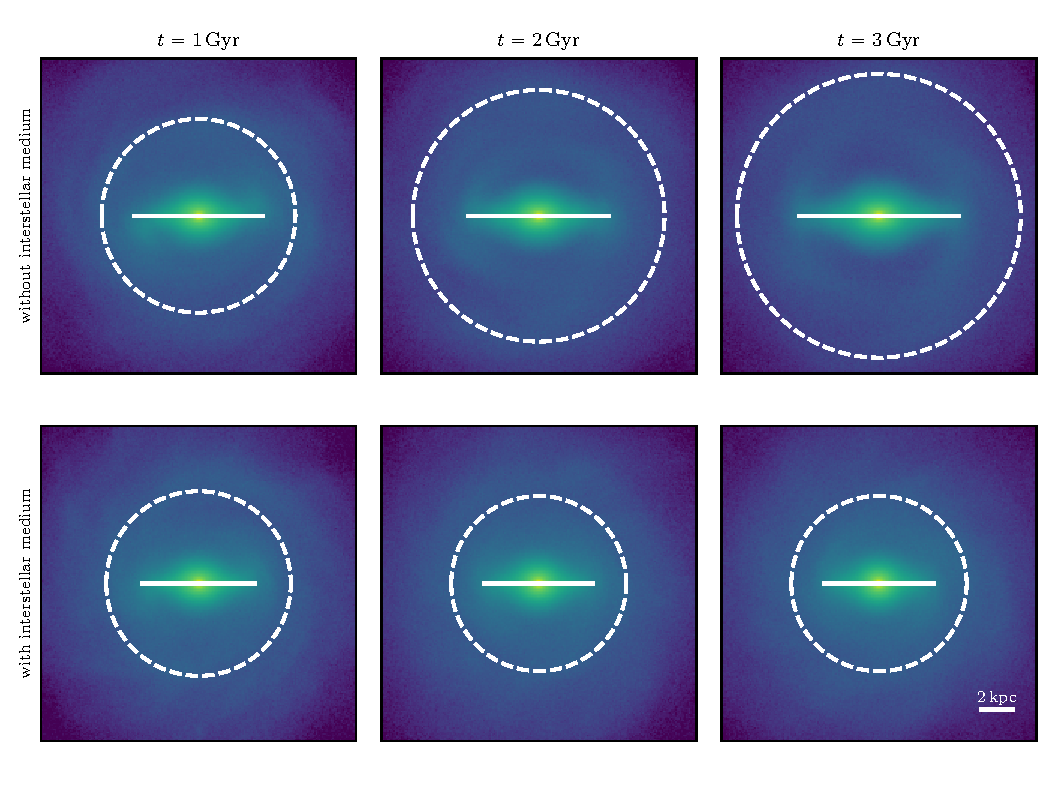
\includegraphics[width=\textwidth]{fig/fig1.pdf}
    \caption{Stellar mass distribution of our simulations with and without
    the interstellar medium. The upper panels show an \Nbody{} only simulation
    while the lower panels show a simulation which includes the \SMUGGLE{} model
    for the interstellar medium. Each panel is $20\,\textrm{kpc}$ to a side.
    The bar length is shown as a solid white bar (details on its
    computation are given in the text). The corotation radius is shown as a
    dashed white circle. Columns show different points in time, separated by
    $1\,\textrm{Gyr}$. We can see that in the \Nbody{} run, the bar grows in
    length and strength. In the \SMUGGLE{} run, the bar remains at approximately
    the same length and strength over the course of the simulation. The \Nbody{}
    model is identical to the GALAKOS model (with different particle
    numbers and softening lengths), discussed in the text.}\label{ch2:fig:overview}
\end{figure*}

Approximately two-thirds of spiral disks host an elongated bar-like feature at
their centers \citep{2000AJ....119..536E, 2007ApJ...657..790M}, including our
own Milky Way \citep{1957AJ.....62...19J, 1991ApJ...379..631B}. The ubiquity of
bars is not difficult to explain, since stellar disks simulated in isolation
almost always form bar-like structures \citep{1971ApJ...168..343H}. Several
studies have shown that a hot, centrally concentrated mass distribution,
such as a stellar bulge or dark matter halo, acts to stabilize stellar disks
against bar formation \citep[e.g.,][]{1973ApJ...186..467O, 1976AJ.....81...30H}.

It is more difficult to reconcile numerical simulations with the observed
pattern speeds of extragalactic bars. Currently, the best technique for
measuring the pattern speeds of individual galaxies is the Tremaine-Weinberg
method \citep{1984ApJ...282L...5T, 2011MSAIS..18...23C}. This approach has
recently been applied to samples of galaxies from the MaNGA survey
\citep{2019MNRAS.482.1733G, 2020MNRAS.491.3655G} and CALIFA survey
\citep{2015A&A...576A.102A}. These studies confirm what was found in earlier
works, that nearly all extragalactic bars are fast rotators (i.e., they rotate
close to their maximum rotation rate).

This is a problem for theoretical simulations, for which there is ample evidence
that galactic bars should resonantly interact with the dark matter halo, causing
the bar to slow down over time \citep{1981A&A....96..164C, 1992ApJ...400...80H,
2000ApJ...543..704D, 2002MNRAS.330...35A, 2002ApJ...569L..83A,
2003MNRAS.341.1179A, 2003MNRAS.346..251O, 2005MNRAS.363..991H,
2006ApJ...637..214M, 2007MNRAS.375..460W, 2009ApJ...697..293D}. The physical
mechanism of this interaction can be understood as an angular form of dynamical
friction between the bar and the dark matter halo. While studied in detail for
the bar \citep{1984MNRAS.209..729T, 1985MNRAS.213..451W}, this process is
generic for any non-axisymmetric disturbance \citep{1972MNRAS.157....1L}. (For
an old but still useful review of bar dynamics, see
\citet{1993RPPh...56..173S}.)

Bar pattern speeds are usually measured using the parameter $\Rot=\RCR/\Rb$,
where \RCR{} is the corotation radius and \Rb{} is the bar length.\footnote{The
radius of corotation \RCR{} is defined for circular orbits as the radius at
which the orbital frequency is equal to the pattern speed, \PS{}, of a given
non-axisymmetric feature. In a galaxy with a constant circular velocity \Vc{},
it is given by $\RCR = \Vc / \PS$.} Bars with $\Rot < 1.4$ are considered
``fast rotators'' while bars with $\Rot > 1.4$ are considered ``slow
rotators'' \citep{2000ApJ...543..704D}. Bars with $\Rot < 1$ are not
thought to be stable \citep{1980A&A....81..198C}. Observational estimates of the
pattern speeds of bars indicate that nearly all galaxies have $1 < \Rot < 1.4$
\citep{2011MSAIS..18...23C, 2015A&A...576A.102A, 2019MNRAS.482.1733G,
2020MNRAS.491.3655G}. We note that \citet{2017ApJ...835..279F} argue that the
pattern speed should be measured relative to a characteristic angular velocity
of the outer disk.

While the fact that a bar is slowed down by a dark matter halo is
well-understood theoretically, this is not the case for the interaction between
a bar and a gaseous disk. Some argue that the gas disk should slow down the bar
more \citep{2003MNRAS.341.1179A}, while others argue that the tendency of the
bar to drive gas inwards means the bar should speed up due to the effect of the
gas disk \citep{2013MNRAS.429.1949A, 2014MNRAS.438L..81A}. Since the gas phase
typically contributes only about $10-20\%$ of the mass of a galaxy at the
present day, one might naively expect it to have a subdominant effect on the
bar. However, because gas is collisional, it can participate in non-resonant
angular momentum exchange with the bar \citep{2011MNRAS.415.1027H}. Thus,
numerical work has shown that the gas phase can have a stronger influence on a
bar than its contribution to the mass of a galaxy would suggest
\citep[e.g.,][]{2010ApJ...719.1470V, 2013MNRAS.429.1949A}.


In the last decade, stellar bars have been studied mainly in the context of the
instability processes that lead to their formation and their ability to drive
gas toward the galaxy center and contribute to the formation of supermassive
black holes (SMBH). The primary interest of these studies mainly was in the loss
of angular momentum of the gas and the associated  gaseous flow down to the
inner disk, possibly forming a central mass concentration
\citep{2010ApJ...719.1470V}, and fueling the central SMBH
\citep[e.g.][]{1989Natur.338...45S, 1990Natur.345..679S}. A revisit of the more
general problem of galactic bar properties and formation, including the case of
disk galaxies with very large gas fraction is timely since it is clear now that
galactic disks show massive bars already at redshift $z>2$
\citep{2022arXiv221008658G}. At that time the universe was 2.5 billion year old
and galaxies might have as high gas fraction as 80\% \citep{2020ARAA..58..157T}.
Furthermore, unlike nearby disk galaxies, the high-redshift disks also
continuously accrete cold gas from the cosmic web, making the formation,
stability and evolution of non-axisymmetric features a key question to address
since they can play a fundamental role in the more general problem of disk
galaxy evolution.



We have performed a simulation of a disk galaxy using the finite-volume,
gravito-hydrodynamics code \AREPO{} \citep{2010MNRAS.401..791S}. We use the
galaxy formation model Stars and MUltiphase Gas in GaLaxiEs
\citep[\SMUGGLE{};][]{2019MNRAS.489.4233M}. This disk galaxy exhibits almost no
evolution in the bar pattern speed over several Gyr when the gas phase is
accounted for and robustly modeled. This behavior has been observed in
previous works \citep{1993A&A...268...65F, 2007ApJ...666..189B,
2009ApJ...707..218V, 2010ApJ...719.1470V, 2014MNRAS.438L..81A}. We propose a new
physical explanation for this stable behavior.

In particular, we find that the presence of a gas phase in a barred
galaxy can arrest the process by which the dark matter halo brakes the bar. The
constant positive torque on the bar by the gas causes the bar's resonance to
reside in regions which have become depopulated. In the halo wake picture, this
is equivalent to no new material being available to reinforce the wake. We show
that this occurs in a Milky Way-like disk with gas fractions as low as
about $5\%$.

We show stellar mass distributions of our barred galaxy in a case with and
without gas in Fig.~\ref{ch2:fig:overview}. We see that the bar grows longer and
stronger without gas (bar length shown as a white bar), while it remains
at approximately the same length and strength when gas is included. As the
bar without gas slows down, the corotation radius (white dashed circle) grows
larger with time.

% In this work, we present a simulation of an isolated, gas-rich disk galaxy. Our
% galaxy exhibits some similarities to the Milky Way, described in more detail in
% Section XX. Surprisingly, we find that the pattern speed of the bar in this
% galaxy is constant with time. We find that with even modest gas fractions of
% about 5\%, our isolated galaxy displays no evolution in pattern speed over many
% $\textrm{Gyr}$. 

In Section~\ref{ch2:sec:methods}, we describe our initial setup, numerical model,
and details on our bar analysis procedures. In Section~\ref{ch2:sec:results}, we
summarize the main results from our findings. We discuss these findings at more
length and in the context of previous research in Section~\ref{ch2:sec:discussion}
before concluding in Section~\ref{ch2:sec:conclusions}.

% The expectation that a dark matter halo acts to slow down a bar is in conflict
% with observational estimates of bar pattern speeds. Bar rotation rates are
% typically classified by the dimensionless ratio
% % \begin{equation}
% % \Rot = \RCR/R_b\textrm{,}
% % \end{equation}
% where \RCR{} is the radius of corotation and $R_b$ is the length of the
% bar.\footnote{The radius of corotation \RCR{} is defined for circular orbits as
% the radius at which the orbital frequency is equal to the pattern speed,
% $\Omega_p$, of a given non-axisymmetric feature. In a galaxy with a constant
% circular velocity $V_c$, it is given by $\RCR = V_c / \Omega_p$.} Galaxies with
% $\Rot < 1.4$ are considered ``fast rotators'' while galaxies with $\Rot > 1.4$
% are considered ``slow rotators''\cite{2000ApJ...543..704D}. Galaxies with $\Rot
% < 1$ are not thought to be stable\cite{1980A&A....81..198C}. Observational
% estimates of the pattern speeds of bars indicate that nearly all galaxies have
% $1 < \Rot < 1.4$\cite{2011MSAIS..18...23C, 2015A&A...576A.102A,
% 2019MNRAS.482.1733G, 2020MNRAS.491.3655G}.

% The role of gas on the evolution of the bar is less well-understood. Since the
% gas phase typically only contributes about $10-20\%$ of the mass of a galaxy at
% the present day, one might naively expect it to have a subdominant effect on the
% bar. However, because gas is collisional, it can participate in non-resonant
% angular momentum exchange with the bar\cite{2011MNRAS.415.1027H}. Thus,
% numerical work has shown that the gas phase can have a stronger influence on a
% bar than its contribution to the mass of a galaxy would
% suggest\cite{2010ApJ...719.1470V, 2013MNRAS.429.1949A}.

\section{Methods}
\label{ch2:sec:methods}
\begin{figure}
    \centering
    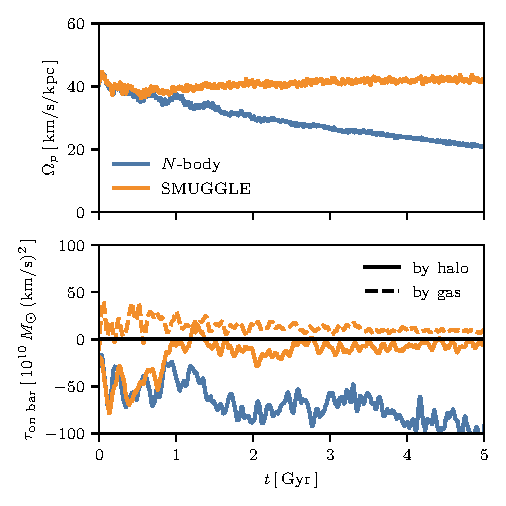
\includegraphics[width=208.14452628pt]{fig/ps_torque.pdf}
    \caption{The \textit{upper panel} shows the evolution of the pattern speed.
    As expected, the bar in the \Nbody{} run slows down due to interactions
    between the bar and the dark matter halo. However, the bar in the \SMUGGLE{}
    run does not slow down and instead remains at a constant pattern speed. The
    \textit{lower panel} shows the torque on the bar by different components.
    The solid lines indicate the torque exerted by the halo in both the \Nbody{}
    and \SMUGGLE{} cases. The dashed line is the torque exerted by the gas phase
    in the \SMUGGLE{} run (there is no gas in the \Nbody{} run). After
    $\sim1\,\textrm{Gyr}$ of evolution, the torque by the halo in the \SMUGGLE{}
    case is severely reduced. We call this bar locking, and discuss its proposed
    origin in Section~\ref{ch2:sec:discussion}. Details on the calculation of the
    torque and pattern speed is given in
    Section~\ref{sch2:sec:bar_analysis}.}\label{ch2:fig:prop}
\end{figure}

\begin{figure}
    \centering
    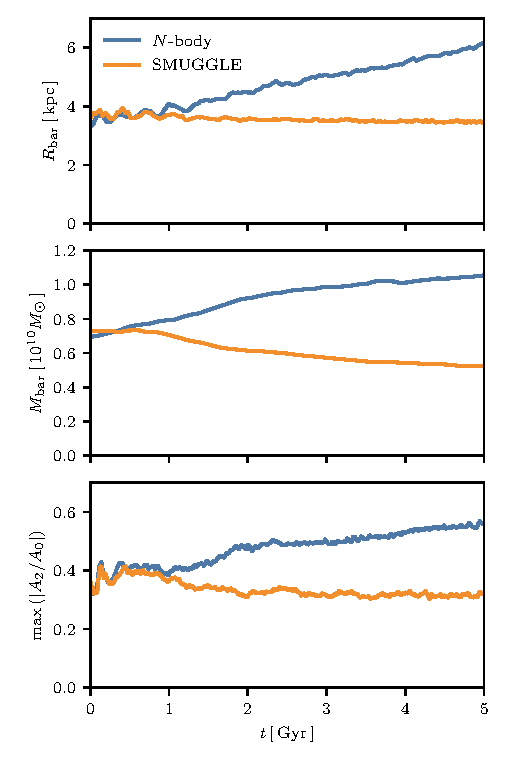
\includegraphics[width=9cm]{fig/Rb_A2.pdf}
    \caption{The evolution in bar length, mass and strength. The \textit{upper panel}
    shows the evolution of the bar length. In the \Nbody{} case, the bar
    lengthens. This occurs because as the pattern speed drops, bar-like orbits
    at larger radii are possible. Stars are captured on these orbits,
    lengthening the bar. This process does not occur in the \SMUGGLE{} cases
    since the bar pattern speed is not decreasing, and therefore the bar length
    remains constant. The bar mass, shown in the \textit{middle panel}, is
    increasing in the \Nbody{} case as the bar grows. It is decreasing in the
    \SMUGGLE{} case, indicating mass redistribution without a change in
    pattern speed. The bar strength, shown in the \textit{lower panel} is
    measured as the maximum of the second Fourier component divided by the
    zeroth Fourier component. We see that in the \Nbody{} case (blue) the bar
    strength increases with time, consistent with previous results showing that
    the bar strength increases as bars slow down. In the \SMUGGLE{} case
    (orange), we see that the bar strength slightly decreasing with time. This
    is also consistent with the expected relation between pattern speed and
    strength since the bar in this case is not slowing down.}
    \label{ch2:fig:strength}
\end{figure}
\subsection{Initial Conditions}
The initial setup of the galactic disk used in this work follows closely the
GALAKOS model \citep{2020ApJ...890..117D}, which uses a modified version of the
\texttt{MakeNewDisk} code \citep{2005MNRAS.361..776S}. The GALAKOS model has
three components - a radially exponential and vertically isothermal stellar
disk, and a stellar bulge and dark matter halo following a Hernquist profile
\citep{1990ApJ...356..359H}. All \Nbody{} runs in this work used the same setup
parameters as the GALAKOS disk, more details of which can be found in the
original paper.

The addition of the gas phase was done as follows. The version of
\texttt{MakeNewDisk} used for the original GALAKOS model can generate a gas disk
which is radially exponential and in vertical gravito-hydrodynamic balance. We
modified the radial profile of this code in order to allow us to generate a disk
with a constant surface density within some cut-off radius, and then
exponentially declining beyond that radius with the scale-length of the stellar
disk. Our fiducial model used an initial surface density of
$20\,M_{\odot}/\textrm{pc}^2$ and a cut-off radius of $9.3\,\textrm{kpc}$.
This corresponds to an initial gas fraction of $\sim16\%$. The initial gas disk
is generated with a temperature of $10^4\,\textrm{K}$ and solar metallicity.

After generating the gaseous disk in this way, we stitched the gas disk together
with the GALAKOS \Nbody{} disk (and bulge and dark matter halo) after the
GALAKOS disk has been allowed to evolve for $1.5\,\textrm{Gyr}$. The purpose of
allowing the GALAKOS disk to evolve first for a short period of time is to allow
for the bar to form unimpacted by the presence of the gas. We found that
including the gas before the bar has formed disrupts the formation of the bar,
as has been seen previously \citep[e.g.,][]{2013MNRAS.429.1949A}. Throughout
this work, we consider $t=0$ for the \Nbody{} run to be the time at which we
added the gas phase for the \SMUGGLE{} run (i.e., we ignore the first
$1.5\,\textrm{Gyr}$ of evolution of the \Nbody{} disk when the bar is forming).

We made one additional modification when stitching the gas disk together with
the \Nbody{} disk - we created a hole within the central $4\,\textrm{kpc}$ of
the gas disks. This hole guards against an initial dramatic infall of gas within
the bar region, which we found to destroy the bar. It is not uncommon for
observed barred galaxies to have gas deficits in the bar region \citep[though
not in the very center;][]{1993RPPh...56..173S}. Therefore, our practice of
allowing the gas distribution to have a hole in the central region is consistent
with our choice to begin the simulations with a bar already formed. In this
manner, we are able to study the ensuing self-consistent interaction between the
bar and the gas, but of course we are unable to explore the origin of bars in
the presence of the gas.

Our method for initializing gas was arrived at after numerous attempts to
include enough gas in the simulation to be compatible with the Milky Way while
also not destroying the bar. For example, we tried evolving an exponential gas
disk adiabatically with the barred disk (i.e., no cooling, star formation, or
feedback). Because there is no mechanism to remove gas from the central region,
a large, highly pressurized pileup of gas forms in the center.\footnote{ We
noticed that the bar slows down in this adiabatic model which lacks a mechanism
to remove gas from the central region. \citet{2007ApJ...666..189B} also noted
slowdown behavior in models which lacked central gas removal. It appears that
gas removal from the center (in our model due to star formation) is necessary to
stabilize a bar's pattern speed.} We then turned on the full SMUGGLE model. As
a result, there is a sudden collapse of gas to the center as pressure support is
lost due to cooling and star formation. This abrupt change in the potential
destroys the bar. 

We don't believe our method is the only nor even the best way to include gas.
One advantage of our method, though, is that it approximates the expectation
that in the bar region the gas surface density should be significantly reduced
\citep[e.g.][]{1993RPPh...56..173S}

We used a mass resolution of $7.5\times10^3\,M_{\odot}$ for the baryonic
components (initial stellar disk, stellar bulge, and gas) and a mass resolution
of $3.75\times10^4\,M_{\odot}$ for the dark matter halo. This mass resolution is
closest to ``level 3'' in the AURIGA simulations \citep{2017MNRAS.467..179G}.
This corresponds to approximately $6.4\times10^6$ particles in the stellar disk,
$1.1\times10^6$ in the bulge, $1.2\times10^6$ in the gas disk, and
$25.3\times10^6$ in the dark matter halo. We used a softening length of
$20\,\textrm{pc}$ for all collisionless components. This softening length is
smaller than used in the original GALAKOS model ($28\,\textrm{pc}$ in their
model, but $\sim43.5\,\textrm{pc}$ when scaled to our mass resolution). Our
smaller softening length is consistent with other resolved ISM models
\citep{2018MNRAS.480..800H, 2019MNRAS.489.4233M}. However, as a consistency
check, we reran our fiducial SMUGGLE run with $40\,\textrm{pc}$ softening and
found no difference in the pattern speed evolution of the bar. For the gas
component, the softening length is fully adaptive with a softening factor of
$2.5$ \citep[e.g.,][]{2020ApJS..248...32W}. Snapshots were saved at equal
intervals of $0.005$ in the time units of the simulation,
$\textrm{kpc}/(\textrm{km}/\textrm{s})$.

Our setup is initially out of equilibrium, but we found that after about
$500\,\textrm{Myr}$, the system has settled into a roughly steady-state
configuration and initial transients appear not to affect the results after this
point. The constant surface density of the initial gas disk is important for
ensuring that the gas disk is dense enough in order for comparisons to real
galaxies to be appropriate.

\subsection{Numerical Model}
We use the Stars and MUltiphase Gas in GaLaxiEs (\SMUGGLE{}) model
\citep{2019MNRAS.489.4233M} implemented within the moving-mesh, finite-volume
hydrodynamics and gravity code \AREPO{} \citep{2010MNRAS.401..791S}. The \SMUGGLE{}
model additionally includes radiative heating and cooling, star formation, and
stellar feedback. Explicit gas cooling and heating of the multi-phase
interstellar medium is implemented, covering temperature ranges between $10$ and
$10^8\,\textrm{K}$.

Star formation occurs in cells above a density threshold
($n_{\textrm{th}}=100\,\textrm{cm}^{-3}$) with a star-formation efficiency of
$\epsilon = 0.01$. Star formation converts gas cells into star particles which
represent single stellar populations with a Chabrier initial mass function
\citep{2003PASP..115..763C}. For each star particle, the deposition of energy,
momentum, mass, and metals from stellar winds and supernovae is modeled.
Photo-ionization and radiation pressure are handled using an approximate
treatment. A more detailed description of this model can be found in the
flagship \SMUGGLE{} paper \citep{2019MNRAS.489.4233M}. A pedagological
review of cosmological simulations of galaxy formation can be found in
\citet{2020NatRP...2...42V}.

We used the fiducial model parameters, except that we increased the number of
effective neighbors $N_{\textrm{ngb}}$ for the deposition of feedback from $64$
to $512$. We found that a lower value of $N_{\textrm{ngb}}$ resulted in
inefficient photo-ionization feedback since the photo-ionizing budget had not
been exhausted after deposition into $64$ neighboring cells. We also employed an
updated version of \SMUGGLE{} using a new mechanical feedback routine similar to
the one described in \citet{2018MNRAS.480..800H}. This updated routine is a
tensor renormalization which ensures linear and angular momentum conservation to
machine precision.

In addition to the \SMUGGLE{} model, we considered a simpler model of the
interstellar medium based upon \citet{2003MNRAS.339..289S}. In this approach,
the multiphase nature of the interstellar medium is described in a subgrid
manner by allowing each resolution element to have a ``cold'' and ``hot''
component, with the equation of state of the gas suitably modified. Gas is
allowed to interchange between the cold and hot components through processes
such as cooling and stellar feedback. Cold gas is allowed to undergo star
formation. We refer to this model as the smooth interstellar medium model, and
it is described in more detail in \citet{2019MNRAS.489.4233M}.

\subsection{Bar Analysis}
\label{sch2:sec:bar_analysis}
The analysis of various bar properties is performed as follows. First, the
pattern speed is measured from the angle of the second Fourier component. We
measured the second Fourier component by computing,
\begin{equation}
\begin{split}
A_2 &= \sum_i m_i e^{i 2 \phi_i} \\
A_0 &= \sum_i m_i \textrm{,}
\end{split}
\end{equation}
where $m_i$ and $\phi_i$ are the mass and azimuthal angle of each particle,
respectively. We computed $A_2$ and $A_0$ in cylindrical bins of width
$0.5\,\textrm{kpc}$ from radii of $0$ to $30\,\textrm{kpc}$. We defined the
angle of the bar $\phi_b$ to be half the angle of the complex number $A_2$
as measured in the bin extending from a radius of $2.5$ to $3\,\textrm{kpc}$.
After correcting for the periodicity of $\phi_b$, we measured the pattern speed
as one-half the two-sided finite gradient of $\phi_b$ as a function of time.
We note that using the second Fourier mode is a blunt tool, discussed in
\citet{2019arXiv190308203P}.

In order to compute other properties of the bar, it is necessary to decompose
the disk into a barred and unbarred component. We achieved this by following
closely the methods described in \citet{2016MNRAS.463.1952P,
2021MNRAS.500..838P}. Our implementation is described in more detail in
Appendix~\ref{ch2:app:bardecomp}. After the disk has been decomposed into a trapped
and untrapped component, we measured the bar length as being the radius $R_b$
which encapsulates $99\%$ of the stars identified as being trapped in the bar.

To compute torques we used the tree algorithm in \texttt{MakeNewDisk}
\citep{2005MNRAS.361..776S} customized to be accessible from \texttt{Python}
using \texttt{Cython}. This algorithm is based on the \texttt{TREESPH} code
\citep{1989ApJS...70..419H}. We constructed a tree with an opening angle of
$0.35$ using only the star particles identified as being trapped in the bar. We
then queried the tree at the locations of all resolution elements in the other
components and computed the torque of the bar on such components. The torque on
the bar by the other components is simply the negative of the torque on the
other components by the bar. A similar analysis using basis function expansions
was performed in \citet{2019MNRAS.490.3616P}.

\subsection{Plotting Details}
We saved snapshots in intervals of $0.005$ in the time units of the simulation,
$\textrm{kpc}/(\textrm{km}/\textrm{s})$, which is very nearly equal to
$1\,\textrm{Gyr}$ (it is $\sim0.977\,\textrm{Gyr}$). Therefore, throughout this
work we referred to the native code time unit as $\textrm{Gyr}$. None of our
results are sensitive to this choice. We applied a Savitzky-Golay filter
\citep{1964AnaCh..36.1627S} as implemented in \texttt{scipy} using a window
length of $21$ and polynomial order of $3$ to the plot of torques
(Fig.~\ref{ch2:fig:prop} and Fig.~\ref{ch2:fig:sam-torque}) and angle differences
(Fig.~\ref{ch2:fig:wake}) in order to remove some numerical noise.

\begin{figure}
    \centering
    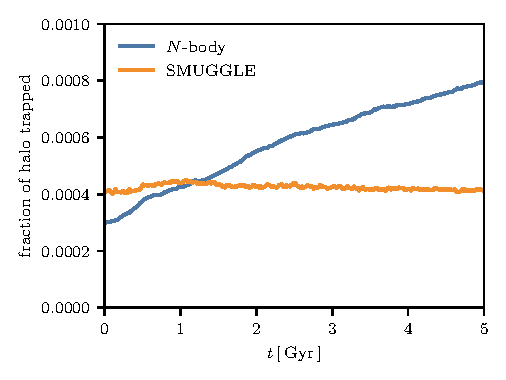
\includegraphics[width=208.14452628pt]{fig/halo_trapped.pdf}
    \caption{The halo mass fraction within two disk scale lengths
    ($\sim5.3\,\textrm{kpc}$) trapped in the \Nbody{} and \SMUGGLE{} runs. As
    the dark matter halo torques the bar, material from the halo is trapped on
    bar-like orbits. In the \Nbody{} case, the trapped fraction increases with
    time, indicating the torquing process is active and the bar is unlocked. In
    the \SMUGGLE{} case, the trapped fraction is nearly constant with time,
    indicating the torquing process is inactive and the bar is locked.}
    \label{ch2:fig:htrap}
\end{figure}

\begin{figure*}
    \centering
    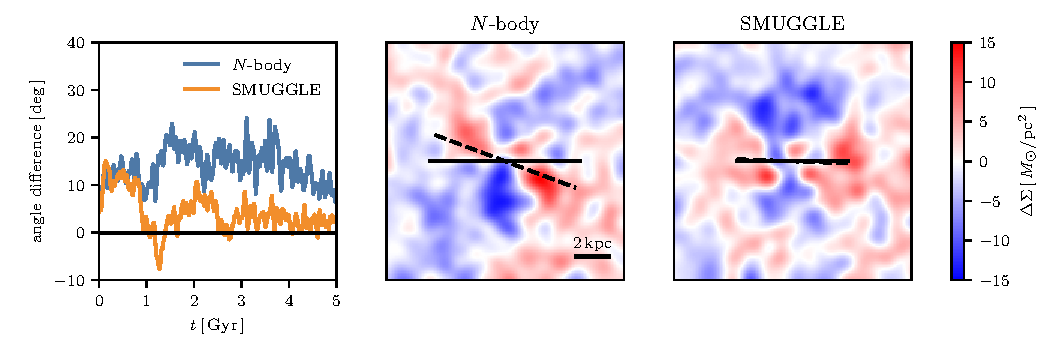
\includegraphics[width=\textwidth]{fig/halo_wake.pdf}
    \caption{The wake excited in the dark matter halo. The dark matter halo wake
    is shown in the \Nbody{} case (\textit{middle panel}) and \SMUGGLE{} case
    (\textit{right panel}) after $2.6\,\textrm{Gyr}$ of evolution. The
    \textit{middle} and \textit{right panels} show a surface density projection
    in the $x$-$y$ plane of the dark matter halo after an axisymmetric average
    has been subtracted. The solid line indicates the direction of the bar while
    the dashed line indicates the direction of the halo wake (both measured by
    taking the second Fourier component within a sphere of all material within a
    radius of $4\,\textrm{kpc}$). The \textit{left panel} shows the time
    evolution of the angle difference between the bar and the halo wake, as
    measured from the second Fourier component. After the first Gyr, the angle
    difference in the \SMUGGLE{} case is smaller than in the \Nbody{} case by about
    a factor of two, reflecting how the dark matter halo in the \SMUGGLE{} case is
    unable to exert as negative a torque on the bar as in the \Nbody{} case.}
    \label{ch2:fig:wake}
\end{figure*}

\section{Results}
\label{ch2:sec:results}

We present the time evolution of different bar properties in Fig.~\ref{ch2:fig:prop}.
In the upper panel, we show the pattern speed over time in the \Nbody{} (blue)
and \SMUGGLE{} (orange) runs. The pattern speed in the \Nbody{} case slows down
while the pattern speed in the \SMUGGLE{} case remains roughly constant. The
slowing down of the pattern speed in the \Nbody{} case is consistent with a long
line of numerical research on bars in \Nbody{} simulations
\citep{1992ApJ...400...80H, 2000ApJ...543..704D, 2002MNRAS.330...35A,
2002ApJ...569L..83A, 2003MNRAS.341.1179A, 2003MNRAS.346..251O,
2005MNRAS.363..991H, 2006ApJ...637..214M, 2007MNRAS.375..460W,
2009ApJ...697..293D}.

However, in the \SMUGGLE{} case the pattern speed remains constant. After the first
Gyr of evolution, we find that the pattern speed increases by only $\sim10\%$
over the next $4\,\textrm{Gyr}$, compared to a $\sim43\%$ decrease in the
pattern speed for the \Nbody{} run over the same interval.

The bottom panel of Fig.~\ref{ch2:fig:prop} shows the torque exerted on the bar by
different components. The solid lines indicate the torque on the bar by the dark
matter halo, whereas the dashed line is the torque on the bar by the gas phase.
In the \Nbody{} case, the halo exerts a steady negative torque on the bar, with
an average torque from $1$ to $4\,\textrm{Gyr}$ of $-58.0$ in units of
$10^{10}M_{\odot}\,(\textrm{km}/\textrm{s})^2$. The halo in the \SMUGGLE{} case
exerts a similar negative torque on the bar in the first Gyr of evolution, but
after that the halo exerts a much weaker torque on the bar, averaging only
$-7.8$ in the same units and over the same time interval. The gas in the \SMUGGLE{}
case exerts a steady positive torque averaging $11.7$ over $1\,\textrm{Gyr}$ in
the same units.

As we saw qualitatively in Fig.~\ref{ch2:fig:overview}, the upper panel of
Fig.~\ref{ch2:fig:strength} shows that the length of the bar in the \Nbody{} case
grows over time while it remains roughly constant in the \SMUGGLE{} case. This
is also consistent with previous numerical work, which found that bars tend to
grow as they slow down and the radius of corotation increases
\citep{2000ApJ...543..704D, 2003MNRAS.341.1179A}. The middle panel of
Fig.~\ref{ch2:fig:strength} shows the mass of the bar. As the \Nbody{} bar slows
down and lengthens, it also grows in mass. The \SMUGGLE{} bar, however, loses
mass over time. This indicates a change in the bar's angular momentum without 
a change in pattern speed, and highlights the
fact that bars are not solid bodies and can respond to external torques through
mass redistribution.

The time evolution of the bar strength, defined as the maximum of
$\left|A_2/A_0\right|$ as a function of radius, is shown in the lower panel of
Fig.~\ref{ch2:fig:strength}. The quantity $\left|A_2/A_0\right|$ varies from $0$ to
$1$, with larger values indicating a stronger bar pattern. We see that in the
\Nbody{} case, $\left|A_2/A_0\right|$ increases over time as the bar pattern
slows. This is consistent with previous \Nbody{} simulations which showed a
clear correlation between the bar pattern speed and the bar strength
\citep[e.g.,][]{2003MNRAS.341.1179A}. In the \SMUGGLE{} case, we see that the
bar strength has an initial drop but then remains at a roughly constant, but
slightly decreasing, strength. This is consistent with the pattern speed in the
\SMUGGLE{} case being roughly constant or slightly increasing.

\section{Discussion}
\label{ch2:sec:discussion}
\subsection{Pattern Speed Evolution}
The lack of evolution in the pattern speed of the \SMUGGLE{} case (seen in
Fig.~\ref{ch2:fig:prop}) is intimately tied to the sudden decrease in torque exerted
on the bar by the dark matter halo. 

%We argue that this can be understood in terms of the halo wake mechanism. 
We interpret this behavior in terms of the halo wake mechanism. In the
\Nbody{} case, a well known phenomenon is that the halo material resonant with
the bar forms a wake, and this wake lags behind \citep{1984MNRAS.209..729T,
1985MNRAS.213..451W, 1992ApJ...400...80H} and exerts a negative torque on the
bar, slowing it down (see Fig.~\ref{ch2:fig:wake} below).\footnote{Since the bar is not a solid
body, it is not guaranteed that a negative torque will slow it down - e.g. a
negative torque could reduce the mass of the bar, reducing its moment of inertia without
changing its pattern speed. However, the bar seems to empirically respond to a
negative torque induced by a halo wake by slowing down.} As the bar slows down,
the location of the resonances in the phase space changes (see Fig.~12 and Table
1 in \citet{2020ApJ...890..117D}) allowing halo material newly resonant with the
bar to participate in the formation of the wake. However, the gas is also a
reliable source of positive torque on the bar, speeding the bar up. In turn,
this stops the location of the resonance from changing such that the halo cannot
reinforce the wake, therefore arresting the process by which the halo can slow
the bar down. We term this process ``bar pattern speed locking,'' or simply
bar locking for short.\footnote{ To be more explicit, it is the gas which locks 
the pattern speed of the bar. The gas does this by forcing the resonant locations 
of the bar into regions of the halo phase space that can no longer support 
significant negative torque.} 

This bar locking process is similar to the ``metastability'' effect, which has
been previously discussed in the literature \citep{2003MNRAS.345..406V,
2006ApJ...639..868S}. Finally, we also note that these authors, in particular,
observe that the effects of numerical resolution in the simulations adopted to
explore these mechanisms have yet to be fully explored and could play a role in
the observed phenomenology of the simulations. We plan to address these issues
in future dedicated work.

We test this interpretation in two ways. First, we measure the fraction of
mass trapped in the halo. As material in the halo wake torques the bar, that
material becomes trapped on bar-like orbits \citep[the ``shadow
bar'';][]{2016MNRAS.463.1952P}. In Fig.~\ref{ch2:fig:htrap} we show the halo trapped
fraction for particles with radii less than two disk scale lengths
($\sim5.3\,\textrm{kpc}$). In the \Nbody{} case, the trapped fraction increases
with time, as expected since the halo is actively torquing the bar (which is,
therefore, unlocked). In the \SMUGGLE{} case, the trapped fraction is constant
(or perhaps slightly decreasing) with time (indicating the bar is locked). This
supports our interpertation that the halo wake process has shut down in the
presence of the gas phase.

Second, we measure the angle offset between the halo wake and the bar. If the
wake and the bar are aligned (i.e., there is no angle offset), then the wake
cannot exert a negative torque on the bar. This angle is plotted in the left
panel of Fig.~\ref{ch2:fig:wake}, which shows that the angle offset is larger in the
\Nbody{} case than in the \SMUGGLE{} case by about a factor of three. The
center and right panels of Fig.~\ref{ch2:fig:wake} show the halo wake with respect
to the location of the bar in the \Nbody{} (center) and \SMUGGLE{} (right) cases
at one point in time. Note that in Fig.~\ref{ch2:fig:wake} we have removed the
halo material trapped in the bar, which exerts no net torque on the bar.

The presence of the gas can arrest the process by which additional material in
the dark matter halo can contribute to a wake. However, this does not explain
why the pattern speed in the \SMUGGLE{} case is nearly constant over several
Gyr. Naively, it would be a coincidence that the bar pattern speed remains
constant in the \SMUGGLE{} case, resulting from a chance cancellation of the
halo and gas torques. However, a constant pattern speed in the presence of gas
has been observed in a few simulations of barred galaxies with gas
\citep{1993A&A...268...65F, 2007ApJ...666..189B, 2009ApJ...707..218V,
2010ApJ...719.1470V, 2014MNRAS.438L..81A}.

\citet{1993A&A...268...65F} argue this behavior is due to the steepening of the
circular velocity curve in the central region as the bar drives gas to the
center. \citet{2009ApJ...707..218V} argue this behavior occurs when the
corotation resonance is larger than the disk radius, but we observe the behavior
when the corotation radius is well within the disk.

% Previous work has argued this is due to the bar torquing
% gas inwards, but no explanation has been given for why it might remain constant.

We propose that an equilibrium mechanism is responsible for the pattern speed
remaining approximately constant. In this scenario, residual negative torque
from the dark matter halo balances out the positive torque from the gas phase.
It has been shown when an analytic bar is forced to rotate at a constant pattern
speed for a few Gyr, the halo exerts almost no torque on the bar
\citep{2022MNRAS.513..768C}. We saw in Fig.~\ref{ch2:fig:prop} that the dark matter
halo in our simulation is still able to support some negative torque over a
several Gyr time span.

We argue that the following occurs. First, the bar is not able to slow down
quickly enough due to the positive torque of the infalling gas. This causes the
resonant halo phase space at a particular pattern speed,
$\Omega_{\textrm{p},0}$, to become mixed and no longer able to support a
negative torque.\footnote{In the halo wake picture, this corresponds to the wake
becoming fully aligned with the bar.} Second, the gas is still exerting a
positive torque on the bar, and therefore the pattern speed will again increase.
Since at higher pattern speeds the halo has not yet been totally mixed,
the halo will once again be able to exert a negative torque on the bar. The
pattern speed will then settle at a new value slightly higher than
$\Omega_{\textrm{p},0}$ where the gas and halo torques cancel. Over time, the
pattern speed should slowly increase.

\subsection{Delayed Gas Injection}
A clear prediction of our proposed mechanism is that the constant pattern speed
a particular galaxy will end up is somewhat arbitrary. In the real universe for
an isolated galaxy it would be the formation pattern speed of the bar while in
our simulation it is the pattern speed of the bar when gas is added to the
system. We tested this by adding gas to the system at a later time when the bar
has further grown and slowed down with time. In our particular test, we added
the gas at a time when the pattern speed is
$\sim30\,\textrm{km}/\textrm{s}/\textrm{kpc}$. As shown in
Fig.~\ref{ch2:fig:snap700}, we find that the pattern speed evolution is very similar
between the two cases (orange and red lines). If anything, the system with a
lower pattern speed seems to speed up more, which is consistent with our picture
since the stronger bar should experience a larger torque from the gas as it is
more efficient at driving gas inflows. We also show in the
Appendix~\ref{ch2:app:varyps} that more slowly rotating bars at fixed bar strength
are more efficient at driving gas inflows as well. Nonetheless, when the initial
pattern speed is lower (red line), the addition of gas does not cause the
pattern speed to quickly return to the higher value of our fiducial simulation
(orange line).



\subsection{Varying Initial Gas Fractions}
We performed a test in which we varied the initial gas fraction of the
disk. In our fiducial run, we set the surface density of the gas disk from
$4\,\textrm{kpc}$ to $\sim9.3\,\textrm{kpc}$ to be $20\,\Msun/\textrm{pc}^2$.
We also ran with surface densities of $15$, $10$, and
$5\,\Msun/\textrm{pc}^2$. These correspond to initial gas fractions of
approximately $16\%$, $10\%$, $7\%$, and $4\%$. The pattern speed evolution is
shown in Fig.~\ref{ch2:fig:fgas}. We find that the bar in disks with
initial surface densities of $20$, $15$, and $10\,\Msun/\textrm{pc}^2$ evolve
with a constant pattern speed while the bar in a disk with initial surface
density of $5\,\Msun/\textrm{pc}^2$ slows down at a similar rate to the \Nbody{} case.

After $5\,\textrm{Gyr}$, the $10\,\Msun/\textrm{pc}^2$ simulation has a gas
fraction of $5.7\%$, but still exhibits constant pattern speed behavior. As a
result, we conclude that for the disk, bar, and halo properties considered in
this work, a gas fraction of only approximately $5\%$ is necessary in order for
the proposed stabilizing mechanism to operate. We stress that this gas
fraction threshold is only for the system considered in this work. Systems with
different structural parameters may require a different threshold. For example,
\citet{2015MNRAS.454.3166A} find slowdown behavior in a barred disk $10$ times
less massive than ours with a gas fraction of $10\%$. To make things more
complicated, \citet{2010ApJ...719.1470V} find that the gas fraction cutoff
varies with the softening length used. Determining exactly how the gas fraction
cutoff varies with these considerations deserves further attention.





\begin{figure}
    \centering
    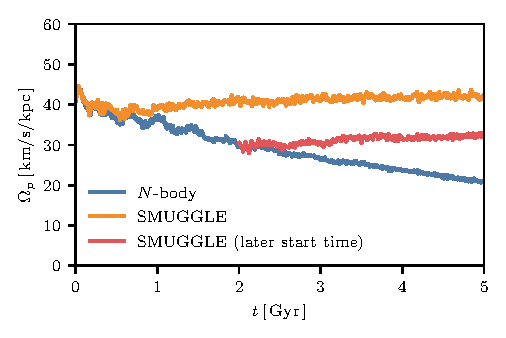
\includegraphics[width=9cm]{fig/ps_late_start.pdf}
    \caption{Pattern speed evolution with a lower initial pattern speed. We
    tested the evolution of our system when gas is added to the \Nbody{} run at
    a later time, but with all other simulation parameters kept the same. The
    setup is therefore identical to our previous runs just with a bar that is
    larger, stronger, and with a lower pattern speed. We find that the pattern
    speed evolution is very similar to our fiducial case, except that the bar
    retains its original pattern speed. This indicates a mechanism which keeps
    the bar at its formation pattern speed, and that there is not a particular
    pattern speed which the system tends to.}
    \label{ch2:fig:snap700}
\end{figure}

\begin{figure}
    \centering
    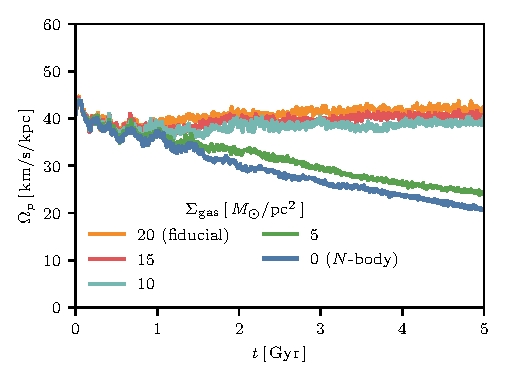
\includegraphics[width=9cm]{fig/ps_fgas.pdf}
    \caption{Pattern speed evolution with varying gas fractions. We explored the
    impact of lowering the initial gas surface density of our fiducial disk on
    the evolution of the pattern speed. The surface densities we tested of $20$,
    $15$, $10$, and $5\,\Msun/\textrm{pc}^2$ correspond to initial gas
    fractions of $16\%$, $10\%$, $7\%$, and $4\%$. We find that initial surface
    densities $20$, $15$, and $10\,\Msun/\textrm{pc}^2$ result in bars which
    remain at a constant pattern speed, while an initial surface density of
    $5\,\Msun/\textrm{pc}^2$ results in a bar which slows down in roughly the
    same manner as the \Nbody{} case.}
    \label{ch2:fig:fgas}
\end{figure}

\subsection{Semi-Analytic Model}
We also developed a simple semi-analytic model of a bar-disk-halo system. This
exercise demonstrates that our proposed mechanism follows from a few simple
assumptions. Our method follows closely the one developed in
\citet{2022MNRAS.513..768C}. We model the bar-disk-halo system with three
components: a dark matter \citet{1990ApJ...356..359H} halo, a
\citet{1975PASJ...27..533M} disk, and a pure quadrupole bar
described in \citet{2022MNRAS.513..768C}. The bar and disk components are just
described by their potential, but we integrate the trajectories of test
particles drawn from a Hernquist halo. Note that we do not include the
interactions between these test particles, and so this model is not
self-consistent. We give our chosen parameter values in Appendix~\ref{ch2:app:sam}.

We allow the bar in this model to rotate as a solid body. However, we crucially
allow the pattern speed of the bar to freely change with time in accordance with
the torque exerted on the dark matter halo by the bar. In particular, we
subtract the $z$-component of this torque divided by the moment of inertia of
the bar from the pattern speed at each timestep. Since the radius of corotation
\RCR{} is a parameter in the bar model from \citet{2022MNRAS.513..768C}, we
allow the moment of inertia of the bar to vary with ${\RCR}^2$. This is
inspired by the fact that the moment of inertia of an ellipsoid scales with the
sum of the square of its axes. To be more precise, we allow
\begin{equation}
I = \frac{I_6}{10^{10} \Msun (\kms)^2} \left( \frac{\RCR}{6\,\textrm{kpc}} \right)^2\textrm{,}
\end{equation}
where $I_6$ is a free parameter chosen by the user. We found that allowing
$I_6=8$ is a good approximation to our fiducial disk model. In code units, the
moment of inertia of the \SMUGGLE{} bar (i.e., the particles classified as being in
the bar) is about $2$. This is a factor of $4$ smaller than our fiducial value
of $I_6=8$, but this is probably due either to the fact that the bar does not
really rotate as a solid body or that resonantly captured stars contribute to
the real bar's effective moment of inertia \citep{1985MNRAS.213..451W}.

In addition to $I_6$, we allowed for another free parameter - the torque from
the gas phase on the bar, $\tau_{\textrm{gas}}$. This torque is applied to the
bar in the same way as the torque from the halo is applied. The torque is given
in code units ($10^{10}\Msun \left(\kms\right)^2$).

We show the effect of varying the gas torque $\tau_{\textrm{gas}}$ from $0$ to
$20$ in increments of $2$ in Fig.~\ref{ch2:fig:sam}. The solid lines indicate the
semi-analytic model, while the two dashed lines correspond to our fiducial
simulations introduced earlier. For reference, the average torque exerted by the
gas phase on the bar in our fiducial simulation was $11.7$ in code units. We see
in Fig.~\ref{ch2:fig:sam} that we can reproduce the stability of our fiducial gas
disk (i.e., its lack of secular evolution) simply by including a positive torque
on the order of $6$. Our semi-analytic model with no gas torque can reproduce
the pattern speed evolution of the $N$-body case.

We next take the $\tau_{\textrm{gas}}=0$ and $20$ cases from Fig.~\ref{ch2:fig:sam}
and plot the halo torque evolution. This result, given in
Fig.~\ref{ch2:fig:sam-torque}, is comparable to the lower panel of
Fig.~\ref{ch2:fig:prop}. We find that the $\tau_{\textrm{gas}}=0$ case compares
favorably to the \Nbody{} case described in previous sections. The bar exerts a
steady negative torque in this case (blue line). When a gas torque is included
(orange lines), we find that the halo's torque becomes much weaker, similar to
what we found in the \SMUGGLE{} case. The gas applies a steady positive torque
by construction. Therefore, the locking process is reproduced in our simple
semi-analytic model. Curiously, we do not see the bimodal behavior in
Fig.~\ref{ch2:fig:fgas} and described in \citet{2010ApJ...719.1470V}. It is not
presently clear why this is the case.

\subsection{Observations}
\label{sch2:sec:observations}
Observational estimates of the pattern speeds of bars indicate that nearly all
galaxies have $1 < \Rot < 1.4$ \citep{2011MSAIS..18...23C, 2015A&A...576A.102A,
2019MNRAS.482.1733G, 2020MNRAS.491.3655G}, where $\Rot$ was defined in
Section~\ref{ch2:sec:intro} to be $\Rot\equiv \RCR/\Rb$. This observational fact has
long been in conflict with the theoretical expectation that bars should slow
down, increasing \Rot{} \citep[e.g.][]{1984MNRAS.209..729T, 1985MNRAS.213..451W,
2000ApJ...543..704D}. Explanations for this discrepancy have been given in the
past. Some have argued that perhaps the central regions of dark matter haloes
are less dense than we expected from $\Lambda\textrm{CDM}$
\citep[e.g.][]{2000ApJ...543..704D,2021A&A...650L..16F}. Some have argued that
perhaps bars are recurrent, short-lived phenomena, and that all the bars we see
in the local universe are very young \citep{2002A&A...392...83B,
2005MNRAS.364L..18B}. Some have argued that modifications to General Relativity
ease the tension between the observed universe and $\Lambda\textrm{CDM}$
\citep[e.g.][]{2021MNRAS.503.2833R, 2021MNRAS.508..926R}.

Because such a small gas fraction is necessary for our stabilizing mechanism to
operate ($5\%$ in our Milky Way-like disk), we argue that most galaxies host a
bar that is not slowing down. This naturally explains why most observed bars are
fast rotators. However, we acknowledge two instances of reported discrepancies
between our mechanism and observations.

First, we note that \citet{2020MNRAS.491.3655G} found that the rotation
parameter \Rot{} positively correlates with gas fraction, such that galaxies
with higher gas fractions are rotating more slowly. However, it is not obvious
this is in tension with our result since the gas fraction of galaxies correlates
with other galactic properties \citep{2009ARAA..47..159B}. Furthermore, the
measurement of pattern speeds is a delicate process still prone to large errors.

Second, the work of \citet{2021MNRAS.500.4710C} and \citet{2021MNRAS.505.2412C}
have made indirect measurements of the deceleration of the bar's pattern speed
from kinematics and chemistry. We point out that these reported measurements are
not direct measurements of the Milky Way bar's deceleration. For instance,
\citet{2021MNRAS.500.4710C} measures the pattern speed based on the asymmetry of
the Hercules stream, but this can also be produced by spiral arms
\citep{2018MNRAS.481.3794H}. Much like the simulations in the present work, the
simulations of these two works do not properly account for the complicated
formation process of the Galactic bar, which may leave imprints on the present
day distribution of stars in spatial, kinematic, and chemical space. More
investigation is necessary to reconcile the present work with these two
well-executed manuscripts.

Lenticular galaxies which lack a signficant gas phase offer an opportunity
to find slowly rotating bars. It would still take several Gyr for a galaxy
hosting a fast bar to transition to the slow bar regime, so slow bars should
only occupy lenticular galaxies which have been lenticular for some time.
NGC~4277 is one such example, whose bar has been found to rotate with
$\Rot{}\sim1.8$ \citep{2022A&A...664L..10B}. On the other hand, NGC~4264 has a
fast bar with $\Rot{}\sim1$ \citep{2019MNRAS.488.4972C}. The difference has been
explained by differences in the dark matter content of the galaxies
\citep{2023MNRAS.521.2227B}. We offer another explanation based on the timing of
when gas was stripped from these galaxies.

There are further examples of gas-rich galaxies hosting slow bars. For
example, UGC~628 \citep[$\Rot\sim2$;][]{2009A&A...499L..25C} and NGC~2915
\citep[$\Rot>1.7$;][]{1999AJ....118.2158B}. UGC~628
has been studied in detail by \citet{2016MNRAS.463.1751C}, who note that it
indeed has a low gas fraction for galaxies of its type. NGC~2915 has a gas
fraction of $70\%$ \citep{2010ApJ...715..656W}, which would seem to be in
conflict with our prediction that only a $5\%$ gas fraction is necessary to
arrest the halo slowdown process. However, NGC~2915 has significantly different
structural properties than the Milky Way-like model we considered in this work.
In particular, it has a signficantly lower mass ($\sim10^9\Msun$ compared to
$4.8\times10^{10}\Msun$ in our model). Further work is necessary to see how the
gas fraction threshold varies with galactic properties.

\citet{2020MNRAS.495.4158F} find that quenched galaxies tend to host longer bars
than star-forming galaxies. This provides some support for our proposed
mechanism since there is evidence quenching can occur through gas depletion
\citep[e.g.][]{2021Natur.597..485W}. However, this correlation could be
explained simply by the fact that longer bars ought to be more efficient at
quenching their host galaxies \citep[e.g][]{2015A&A...580A.116G}.

Finally, we mention the evolution of \Rot{} in our simulation. In the
$N$-body simulation, the bar forms with $\Rot\sim1.6$ at $t=0\,\textrm{Gyr}$,
which is already well within the slow bar regime. After $5\,\textrm{Gyr}$ of
evolution, \Rot{} has risen to $\sim1.9$. In the SMUGGLE simulation, the gas is
added to the $t=0\,\textrm{Gyr}$ snapshot, so it begins with $\Rot{}\sim1.6$. As
expected, after $5\,\textrm{Gyr}$ of evolution \Rot{} is still $\sim1.6$.
However, this relies on our measure of the bar length as being the maximum
radius of all orbits trapped in the bar, which is not an observationally
accessible measure of bar length. One would need to test different
observationally possible bar length estimators, such as ellipse fitting
\citep{1990MNRAS.245..130A, 1999A&AS..140....1M, 2002MNRAS.330...35A,
2006A&A...452...97M, 2009A&A...495..491A, 2015A&A...576A.102A}. This is beyond the
scope of our current work. Nonetheless, our prediction that \Rot{} is stable in
the presence of sufficient gas is robust. Assuming bars form with $\Rot\sim1$,
we predict this should remain the case with further evolution. Why the $N$-body
simulation forms a bar with $\Rot\sim1.6$ is a separate question deserving
further attention.

\subsection{Previous Idealized Simulation Work}
Substantial work has been devoted to the role of gas in bar dynamics. We
discuss this and highlight the novel aspects of the present investigation.

To our knowledge the first work on a barred galaxy with a gas component was
by \citet{1993A&A...268...65F}. They found a stable pattern speed when a
dissipative component was added to the system, with a slight increase in the
pattern speed near the end of their simulation. However, their model was only
evolved for $\sim1\,\textrm{Gyr}$, so it is unclear if their bar exhibits a
stable pattern speed over several Gyr.

\citet{2007ApJ...666..189B} describe a model containing up to $8\%$ gas.
Their disk is similar to ours (though their dark matter halo is a factor of $10$
less massive). They find slowdown behavior up to a gas fraction of $8\%$, with
the finding that higher gas fractions lead to a reduced slowdown. However, for
the models which they show pattern speeds, they do not include star formation or
the removal of gas from the center of their disk. In preliminary work, we found
slowdown behavior in an adiabatic model with similar gas fractions but lacking
any method for removing gas from the central region (in our fiducial SMUGGLE
model this is achieved through star formation). We surmise that the removal of
gas from the central region is an important requisite for stable pattern speeds,
though a careful torque analysis is necessary to confirm this hypothesis.

\citet{2010ApJ...719.1470V} do find stable pattern speeds in models with
gas fractions as low as $8\%$ (depending on the force softening used).
Crucially, their model does contain a routine for removing gas from the central
region of the disk. These authors state the behavior is bimodal, with a clear
stable regime and a slowdown regime. These authors make no mention of the
process by which the halo braking process is arrested, as we propose in the
present paper.

\citet{2013MNRAS.429.1949A, 2014MNRAS.438L..81A} find stable evolution in \Rot{}
for a triaxial halo over $10\,\textrm{Gyr}$ with initial (final) gas fractions
of $100\%$ ($7\%$), $75\%$ ($6\%$), and $50\%$ ($5\%$). For a model with $20\%$
($3\%$) gas fraction they find an increasing \Rot{}. In their model with a
spherical halo they always find increasing \Rot{}, contrary to the present work.
We note there is a structural difference in their dark matter halo. They use a
cored isothermal sphere as opposed to our Hernquist halo. It is not clear to us
the impact this would have on the expected torque from the halo (i.e., the
velocity structure of their halo may allow for more efficient capture and thus
stronger torquing). The bar locking process (or something similar) which we
propose in this paper is not mentioned by these authors.

There may also be issues related to structural differences between their
bars and the bar considered in this work. In our case, we allowed the bar to
form in an $N$-body run and then added gas after the bar formation. In
\citet{2013MNRAS.429.1949A, 2014MNRAS.438L..81A} the bar forms from a disk that
is initially gas-rich. Neither approach is inherently better, but it is known
that in the latter case the resultant bar strength is weaker for initially
gas-rich systems \citep[e.g.,][]{2013MNRAS.429.1949A}. Weaker bars are less
efficient at driving gas inwards \citep{2004ApJ...600..595R} and thus should
experience less positive torque from the gas phase. A direct comparison based on
the torque by the gas phase on the bar is necessary.

\citet{2015MNRAS.454.3166A} describe a model containing gas and stars which
slows down with time. In their model gas is added to the system to target a gas
fraction of $10\%$. However, their disk is about a factor of $10$ less massive
than the disk considered in this work. The necessary gas fraction for a stable
pattern speed probably depends on galaxy properties like mass. It is unclear
whether $10\%$ is sufficient for their bar to have a stable pattern speed.

\subsection{Cosmological Simulations}
Barred galaxies in cosmological simulations of galaxy formation continue to be
in conflict with observations by producing bars which rotate too slowly
\citep{2017MNRAS.469.1054A, 2019MNRAS.483.2721P, 2021A&A...650L..16F,
2022ApJ...940...61F}.\footnote{Though see \citet{2022ApJ...940...61F} who argue
bars have consistent pattern speeds with observations, but are too short.}
These works examine bars in EAGLE \citep{2015MNRAS.450.1937C,
2015MNRAS.446..521S}, Illustris \citep{2014Natur.509..177V,
2014MNRAS.444.1518V}, and Illustris TNG50 \citep{2019MNRAS.490.3196P,
2019MNRAS.490.3234N}. \citet{2015PASJ...67...63O} describe cosmological zoom
simulations of two barred Milky Way-like galaxies that both slow down over time.
As pointed out by \citet{2010ApJ...719.1470V}, the gas fraction cutoff for the
stable pattern speed regime increases with lower softening lengths.
\citet{2015PASJ...67...63O} use softening lengths larger than ours by about a
factor of $6$. This highlights the importance of future work exploring precisely
when barred galaxies ought to be in the stable regime.

\citet{2021A&A...650L..16F} explored the evolution of bars in the Auriga
cosmological zoom simulations \citep{2017MNRAS.467..179G}. They find \Rot{}
values consistent with observations. Furthermore, their pattern speed evolution
shows some apparent periods of stability (see their Fig.~B1). One galaxy, Au26,
appears to even transition from the stable pattern speed regime to the slowing
down regime at a lookback time of $\sim1.8\,\textrm{Gyr}$.

Furthermore, the pattern speeds of bars in both cosmological simulations and the
real universe can be affected by environmental processes not included in our
simulation -- e.g., satellite infall \citep{2011Natur.477..301P}, non-sphericity
\citep{2013MNRAS.429.1949A}, rotation in the dark matter halo
\citep{2013MNRAS.434.1287S, 2014ApJ...783L..18L, 2018MNRAS.476.1331C,
2019MNRAS.488.5788C}, or perhaps even the gaseous circumgalactic medium.
Naturally, extending our present work to account for such effects is a crucial
next step in understanding the formation and evolution of galactic bars. We are
presently engaged in such an exploration.

\begin{figure}
    \centering
    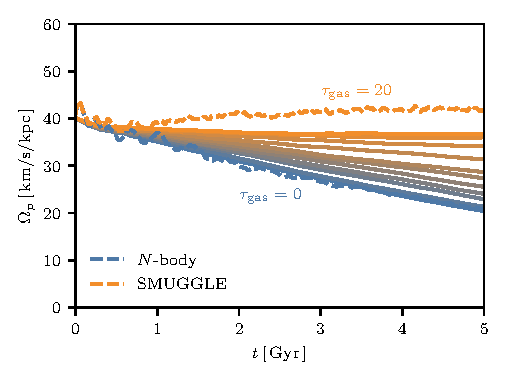
\includegraphics[width=208.14452628pt]{fig/samGvar.pdf}
    \caption{A comparison between the pattern speeds of our fiducial disk
    systems and a semi-analytic model. The solid lines indicate the pattern
    speeds assuming a constant positive torque, varying in increments of $2$
    from $0$ to $20$. The dashed lines indicate the pattern speed evolution from
    our fully self-consistent simulations from earlier. We find excellent
    agreement between our fiducial simulations and our semi-analytic model of a
    bar-disk-halo system. Torques are given in code units ($10^{10}\Msun
    \left(\kms\right)^2$).}
    \label{ch2:fig:sam}
\end{figure}

\begin{figure}
    \centering
    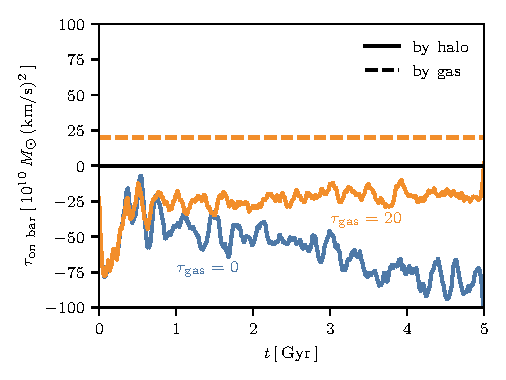
\includegraphics[width=208.14452628pt]{fig/sam_torque.pdf}
    \caption{The torque exerted on the bar by various components in our
    semi-analytic model. Solid lines indicate the torque by the halo while the
    dashed line indicates the torque exerted by the gas phase. We chose two
    models with $\tau_{\textrm{gas}}=0$ and $20$, which most closely resemble
    our $N$-body and \SMUGGLE{} disks, respectively. This figure ought to be
    compared to the lower panel of Fig.~\ref{ch2:fig:prop}. Overall, we find good
    qualitative agreement.}
    \label{ch2:fig:sam-torque}
\end{figure}

\section{Conclusions}
\label{ch2:sec:conclusions}
We performed a simulation of a Milky Way-like galactic disk hosting a strong bar
with a state-of-the-art model for the interstellar medium. We found that the
pattern speed of the bar in this simulation does not slow down but rather
remains at a stable, constant pattern speed. We provided a simple semi-analytic
model which reproduces many of the features from our fiducial disk model.

The implications of our findings are numerous. First, we naturally explain why
nearly all observed galaxies are fast rotators without requiring the inner
regions of dark matter halos to be underdense \citep{1998ApJ...493L...5D,
2000ApJ...543..704D} or requiring new physics \citep{2021MNRAS.503.2833R,
2021MNRAS.508..926R}. Second, we show that the role of gas is of paramount
importance in studies which attempt to uncover the nature of dark matter from
its effect of slowing down the bar \citep{2021MNRAS.500.4710C,
2021MNRAS.505.2412C}. Third, we provide an explanation for how the Milky Way's
bar could be both long-lived and a fast rotator, of which there is some
observational evidence \citep{2019MNRAS.490.4740B}. And finally, we complicate
the picture of stellar radial mixing expected to sculpt the Milky Way's
disk \citep{2012MNRAS.420..913B, 2015ApJ...808..132H}, a process which relies
upon the pattern speed of the bar to change with time. The radial mixing of
the gas phase induced by the bar, as predicted in \citet{2011MNRAS.415.1027H},
might have implications for the radial metallicity gradients of galaxies. Our
work does not alter expectations for radial mixing induced by spiral arms
\citep{2002MNRAS.336..785S}.

We found that below a certain gas fraction, bars should still be able to slow
down. Therefore, we expect barred spiral galaxies which have been gas-poor for
extended periods of time to be rotating very slowly. We therefore predict that
observations which target such galaxies (e.g., lenticular barred galaxies
\citep{2009ARAA..47..159B}) would find slowly rotating bars.\footnote{This does
not mean that we predict \textit{all} gas-poor galaxies should be slowly
rotating. Indeed, they would need to be gas-deficient for several $\textrm{Gyr}$
before they would be classified as slow rotators.} There does exist
examples of galaxies known to be slow rotators -- the low surface brightness
galaxy UGC~628 \citep{2009A&A...499L..25C}, lenticular galaxy NGC~4277
\citep{2022A&A...664L..10B}, and NGC~2915 \citep{1999AJ....118.2158B}. UGC~628
has been studied in detail by \citet{2016MNRAS.463.1751C}, who note that it
indeed has a low gas fraction for galaxies of its type. NGC~2915 has a gas
fraction of $70\%$ \citep{2010ApJ...715..656W}, which would seem to be in
conflict with our prediction that only a $5\%$ gas fraction is necessary to
arrest the halo slowdown process. However, NGC~2915 has significantly different
structural properties than the Milky Way-like model we considered in this work,
discussed in Section~\ref{sch2:sec:observations}. We predict a general trend that
bars in gas-rich spiral galaxies should rotate quickly while some bars in
gas-poor spiral galaxies should rotate slowly.

\section{Acknowledgments}
We would like to thank Greg~L. Bryan, Neal~J. Evans, Drummond~B. Fielding, Keith
  Hawkins, Jason~A.~S. Hunt, Sarah~M.~R. Jeffreson, Kathryn~V. Johnston,
  Peter~M.~W. Kalberla, Jürgen Kerp, Julio~F. Navarro, Dylan Nelson, Suchira
  Sarkar, Joshua~S. Speagle, Martin~D. Weinberg, and Yanfei Zou for helpful
  discussions. A.B. would like to thank Todd Phillips for helpful discussions.
  Some computations in this paper were run on the FASRC Cannon cluster supported
  by the FAS Division of Science Research Computing Group at Harvard University.
  Resources supporting this work were also provided by the NASA High-End
  Computing (HEC) Program through the NASA Advanced Supercomputing (NAS)
  Division at Ames Research Center. This research has made use of the Spanish
  Virtual Observatory (https://svo.cab.inta-csic.es) project funded by
  MCIN/AEI/10.13039/501100011033/ through grant PID2020-112949GB-I00. A.B. was
  supported by the Future Investigators in NASA Earth and Space Science and
  Technology (FINESST) award number 80NSSC20K1536 during the completion of this
  work. E.D. was partially supported by HST grants HST-AR-16363.001 and
  HST-AR-16602.006-A and by NASA Award NASA 80NSSC22K0761. J.Q. acknowledges
  support from NSF grant AST-2008490. L.V.S. is grateful for financial support
  from NASA ATP 80NSSC20K0566, NSF AST 1817233 and NSF CAREER 1945310 grants.
  P.T. acknowledges support from NSF grant AST-1909933, AST-2008490, and NASA
  ATP Grant 80NSSC20K0502. M.V. acknowledges support through NASA ATP
  19-ATP19-0019, 19-ATP19-0020, 19-ATP19-0167, and NSF grants AST-1814053,
  AST-1814259, AST-1909831, AST-2007355 and AST-2107724.

We have made use of the following software:
{\sc agama} \url{https://github.com/GalacticDynamics-Oxford/Agama}, {\sc
astropy} \citep{astropy:2013, astropy:2018}, {\sc h5py}
\url{http://www.h5py.org/}, {\sc inspector\_gadget}
\url{https://bitbucket.org/abauer/inspector_gadget/}, {\sc joblib}
\url{https://joblib.readthedocs.io/en/latest/}, {\sc matplotlib}
\citep{Hunter:2007}, {\sc numba} \citep{lam2015numba}, {\sc numpy}
\citep{harris2020array}, {\sc scipy} \citep{2020SciPy-NMeth}, {\sc tqdm}
\url{https://tqdm.github.io/}

\chapter{A Metallicity-Dependent Star Formation Gap Splits the Milky Way's \texorpdfstring{$\alpha$}{α}-Sequences\footnote{This chapter originally appeared as Beane,~A., 2024, \arxivaccept{2407.07985}{Rising from the Ashes: A Metallicity-Dependent Star Formation Gap Splits the Milky Way's $\alpha$-Sequences}{Astrophys.~J.}}}\label{ch:GSEgas}
% \begin{minipage}{\linewidth}
  % \raggedright
  % \textit{This chapter originally appeared as Beane,~A., 2024, \arxivaccept{2407.07985}{Rising from the Ashes: A Metallicity-Dependent Star Formation Gap Splits the Milky Way's $\alpha$-Sequences}{Astrophys.~J.}}
% \end{minipage}
% !TEX root = ../ms.tex

\begin{adjustwidth}{.8cm}{0cm}
\textit{Greed seeks results.\\Wisdom seeks understanding.}

\hspace{9cm} -- Sayadaw U Tejaniya
\end{adjustwidth}

\section{Abstract}
    The elemental abundance distribution of stars encodes the history of the gas-phase abundance in the Milky Way. Without a large, unbiased sample of highly precise stellar ages, the exact timing and nature of this history must be \textit{inferred} from the abundances. In the two-dimensional plane of \alphaFe{}-\FeH{}, it is now clear that two separate populations exist -- the low-$\alpha$ and high-$\alpha$ sequences. We propose that a brief ($\sim300\,\Myr$) halt in star formation within a narrow metallicity bin can lead to a bimodal \alphaFe{} distribution at that metallicity, assuming a rapidly declining gas phase \alphaFe{}. Using simulations of an idealized setup of a high-$z$ galaxy merger, we show that the merger with the Gaia-Sausage-Enceladus satellite at $z\sim2$ is one possible way to trigger such a gap in the Milky Way. This mechanism may also operate in non-merger scenarios. We predict a $\sim300\,\Myr$ gap in stellar ages at a fixed \FeH{} where the $\alpha$-bimodality is prominent ($\FeH\lesssim-0.2$).

\section{Introduction} \label{ch3:sec:intro}
% What leads to distribution of heavy elements in a galaxy
Many elements heavier than hydrogen are produced through nuclear fusion in compact objects such as supernovae, dying low mass stars, and neutron star-neutron star mergers \citep[e.g.][]{2023A&ARv..31....1A}. By necessity, stars inherit the constitutive properties of the gas from which they formed. Moreover, the surface abundance of most elements for most stars do not change over most of their lifetime. By analyzing the surface abundances of stars, we can reconstruct the historical gas-phase composition of a galaxy.

The enrichment of the gas-phase of a galaxy is determined by a complicated combination of physical processes - stellar evolution and supernovae, gas accretion, mergers, gas outflows from stellar and active galactic nuclei (AGN) feedback, metal mixing and diffusion, etc. Because the processes which give rise to this distribution are complex, there is almost certainly some structure in the stellar abundance distribution for every galaxy. However, it has only been definitively measured in the Milky Way, with conflicting claims of detection \citep{2023ApJ...956L..14K} and non-detection \citep{2024IAUS..377..115N} in M31.

% Why alpha-elements are important
The distribution of elemental abundances is a high dimensional space \citep[e.g., 32 elements in][]{2024ApJ...961L..41J}. However, this space is highly degenerate, and so the effective number of dimensions is much smaller -- even possibly compressed to just \FeH{} and age \citep{2019ApJ...883..177N}. Two elements have received particular interest - Fe and elements produced by the $\alpha$-process. Type Ia and Type II supernovae are the main contributors of Fe and $\alpha$ enrichment. Fe is broadly produced in both types, and so its abundance is a proxy for the total metallicity of a star. On the other hand, $\alpha$-elements are mainly produced in Type II supernovae. The ratio of $\alpha$-elements to Fe (\alphaFe{}) is then a measure of the relative contributions of Type Ia and II SNe to the enrichment of a parcel of gas, which typically declines with time \citep{1979ApJ...229.1046T,1986A&A...154..279M}. It has therefore become common to compress the high-dimensional abundance space to the two dimensional \alphaFe{}-\FeH{} plane.

% Observed chemical bimodality in the Milky Way
These abundances can be used to decompose the Milky Way's disk, which has a long history dating back to the work of \citet{1983MNRAS.202.1025G}, who noted that the vertical distribution of stellar altitudes is well-fit by a double exponential. This led naturally to a ``thin'' and ``thick'' disk, whose membership can be reasonably determined through kinematics \citep[e.g.][]{2003A&A...410..527B}. It was quickly realized that the thick disk is more $\alpha$-enhanced than the thin disk \citep{1996ASPC...92..307G,1998A&A...338..161F}.

Later studies showed that the disk could be decomposed into high- and low-$\alpha$ sequences without kinematic selection \citep{2011A&A...535L..11A,2012A&A...545A..32A}.\footnote{\citet{2003A&A...410..527B} briefly noted that the thin and thick disk seemed to not overlap in chemistry.} The high-$\alpha$ sequence is older, more centrally compact, and more vertically extended than the low-$\alpha$ sequence \citep{2013A&A...560A.109H,2024IAUS..377..115N}. Although the thick disk is more $\alpha$-enhanced than the thin disk, it is not immediately obvious that the chemical and kinematic separations arise from the same physical process \citep[or that they even exist, see][]{2012ApJ...751..131B}.

% Different explanations of bimodality
Naturally, many different processes that could lead to structure in the abundance plane have been discussed in the literature. An early explanation of the bimodality is based on the two-phase gas infall model \citep{1997ApJ...477..765C,2009IAUS..254..191C,2017MNRAS.472.3637G,2019A&A...623A..60S}. In this model, the thick disk first forms rapidly from an initial infall of gas. Because the typical SFR is high, these stars are $\alpha$-enhanced. In some variants, star formation halts completely before a second supply of pristine gas falls into the Galaxy \citep[][and references therein]{2024arXiv240511025S}. This dilutes the gas supply from which the thin disk forms more gradually, creating a loop feature in the abundance plane. The thin disk is then more $\alpha$-poor because its associated SFR is lower, and in certain scenarios two chemically distinct disks are formed.

A later argument by \citet{2021MNRAS.501.5176K} asserts that the two sequences follow from two phases of gas infall, except driven by stellar feedback instead of cosmological inflow. An initial bursty phase follows from the direct collapse of the gaseous halo. The disk has a high SFR leading to the formation of the high-$\alpha$ sequence. Feedback then halts the inflow, and a slower accretion of high-angular momentum and metal-rich gas commences, forming the low-$\alpha$ sequence.

Another mechanism to generate structure in the abundance plane was pointed out by \citet{2009MNRAS.396..203S}, further developed by \citet{2021MNRAS.507.5882S,2023MNRAS.523.3791C}, and explored by \citet{2011ApJ...737....8L,2021MNRAS.508.4484J}. This model claims that, since stars are thought to migrate from their birth radius, there will be stars throughout the entire disk that formed in the inner disk. These $\alpha$-enhanced stars will then form the high-$\alpha$ sequence. This model and its variants also match some chemodynamic properties of the disk. One salient feature of these models is that the bimodality can result from a smooth star formation history.

Yet another explanation, which also invokes an internal process, is that the formation of clumps at high redshift are responsible for both the chemistry and dynamics of the high-$\alpha$ sequence \citep{2019MNRAS.484.3476C,2020MNRAS.492.4716B,2021MNRAS.502..260B,2023ApJ...953..128G}. Instabilities are thought to form clumps in gas-rich disks, and such clumps are seen at intermediate redshifts \citep[$z\sim2$;][]{2005ApJ...627..632E,2007ApJ...658..763E}. These clumps then self-enrich, forming $\alpha$-enhanced stars. The high-$\alpha$ sequence stops forming once the gas fraction is low enough for the instabilities to no longer arise. This model predicts that the high-$\alpha$ and low-$\alpha$ sequences form simultaneously.

Next, we turn to models which argue the bimodality results from some external influence. Early arguments were made that both the $\alpha$-enhancement of the disk and the thickening of the disk can result from gas-rich mergers \citep{2004ApJ...612..894B,2005ApJ...630..298B,2007ApJ...658...60B,2010MNRAS.402.1489R}.\footnote{See also \citet{2009MNRAS.400.1347C} for an argument invoking semi-analytic models.} These mergers lead to an enhanced SFR which leads to the $\alpha$-enhancement of the thick disk, with \citet{2015A&A...578A..87S} being the first to attempt to explain abundance substructure with a merger.

In cosmological simulations, which naturally include early gas-rich mergers, the situation is not as clear. Early work by \citet{2012MNRAS.426..690B} found a general separation between the thin and thick disk, though other authors found a smooth evolution \citep{2013A&A...558A...9M}. \citet{2018MNRAS.474.3629G} found what they referred to as a chemical dichotomy, and argued that it can come from either gas-rich mergers as described before or a ``compaction'' of the disk (we will return to this point in Section~\ref{ch3:ssec:cosmo}). Other authors highlight the metal content of the infalling gas, stating that the metal-poor gas associated with satellites can suddenly dilute or reset the disk's metallicity \citep{2020MNRAS.491.5435B,2024MNRAS.528L.122C}. This interpretation can also be understood in the framework of the two-infall models.

The merger explanation of the bimodality is highly synergistic with our picture of the hierarchical assembly of the stellar halo \citep{2005ApJ...635..931B}. Indeed, there is strong evidence that the Milky Way underwent a significant merger with the so-called Gaia-Sausage-Enceladus satellite \citep[GSE;][]{2018MNRAS.478..611B,2018Natur.563...85H,2020ApJ...901...48N}. This merger is thought to have occurred $\sim8-10\,\Gyr$ ago \citep[see also][]{2020ApJ...897L..18B}. A merger origin of the abundance bimodality is also attractive because it can simultaneously explain the origin of the kinematic thin and thick disk \citep{1985AJ.....90.2015G,1986ApJ...309..472Q,1993ApJ...403...74Q}.

Claims in the literature on the stellar mass of GSE vary widely. Early estimates argued from $6\times10^8$ up to even $10^{10}\,\Msun$ \citep{2018MNRAS.478..611B,2018Natur.563...85H,2019MNRAS.484.4471F,2019MNRAS.487L..47V,2019MNRAS.488.1235M,2020MNRAS.493.5195D,2020MNRAS.497..109F}. Later estimates have been more conservative ranging from a mass of $2.7\times10^8\,\Msun$ to $10^9\,\Msun$ \citep{2019MNRAS.482.3426M,2020MNRAS.492.3631M,2020MNRAS.498.2472K,2021ApJ...923...92N,2022AJ....164..249H}, and even as low as $1.5\times10^8\,\Msun$ \citep{2023MNRAS.526.1209L}.

In this work, we propose that a brief $\sim300\,\Myr$ interruption in the formation of stars at a given metallicity can lead to the formation of an $\alpha$-abundance bimodality at that metallicity. It is not common to study the star formation rate at a specific metallicity, but dividing the stellar population into narrow abundance populations can be a powerful tool \citep[e.g.][]{2012ApJ...753..148B,2012ApJ...751..131B}.

Our proposal assumes that the gas phase's \alphaFe{} is declining sufficiently rapidly at the time of the interruption. Using a set of idealized simulations which mimic the $z\sim2$ merger between the Milky Way and GSE, we show that such a merger can drive the formation of this gap and thus the bimodality. While we demonstrate this mechanism in the context of a merger scenario, it is important to note that our proposal does not inherently require a merger to induce this metallicity-dependent star formation gap. This scenario predicts a $\sim300\,\Myr$ gap in stellar ages at metallicities where the bimodality exists ($\FeH\lesssim-0.2$).

In Section~\ref{ch3:sec:methods}, we describe our setup. In Section~\ref{ch3:sec:results}, we present in detail the main results of two example simulations before expanding our results to the full suite. In Section~\ref{ch3:sec:discussion}, we discuss and interpret our results, as well as connections to previous and future work, before concluding in Section~\ref{ch3:sec:conclusion}. Throughout this work we refer to the standard native time unit $\kpc/\left(\kms\right)$ as \Gyr{} for convenience.

\section{Methods}\label{ch3:sec:methods}
\subsection{Isolated Setup}\label{ch3:ssec:iso_setup}
\begin{figure}
    \centering
    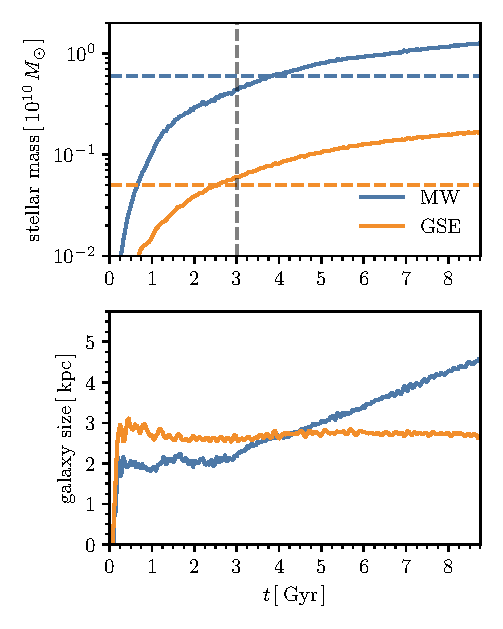
\includegraphics[width=208.14452628pt]{ch3/mass_size.pdf}
    \caption{The mass and size evolution of the central (Milky Way, blue) and satellite (GSE, orange) galaxies simulated in isolation. The mass is taken to be the stellar mass within twice the half-mass radius, and the size is taken to be the half-mass radius. In the upper panel, we also show as a horizontal line the mass of the Milky Way's disk and GSE from the best-fit model of \citet{2021ApJ...923...92N}. This comparison is taken to be made at $3\,\Gyr$ (vertical dashed line), our proxy for $z\sim2$. A precise match is not attempted given the wide ranging uncertainties.}
    \label{ch3:fig:mass_size}
\end{figure}

We use a modified version of the \texttt{MakeNewDisk} variant described in \citet{2023MNRAS.tmp.2070B}. In isolation, each of the central and satellite galaxies are a compound halo setup, with a \citet{1990ApJ...356..359H} dark matter halo and a gaseous halo with a $\beta$-profile:
\begin{equation*}
\rho = \rho_0 \left[1 + \left(\frac{r}{r_c}\right)^2\right]^{-\frac{3\beta}{2}}
\end{equation*}
The total mass within the virial radius is kept fixed, and the mass of the dark matter halo and central density of the gaseous halo are chosen to satisfy a given baryon fraction $f_b$ within the virial radius. The dark matter halo is initialized to be in gravitational equilibrium with the total potential. The gaseous halo is in gravito-hydrostatic equilibrium, where the temperature is allowed to vary as a function of radius. The azimuthal velocity of the gaseous halo is given as a fraction of the circular velocity. There is no initial stellar disk or bulge, and the gas is initially metal-free. Thus, all star particles and metals are formed self-consistently.

\begin{figure}
    \centering
    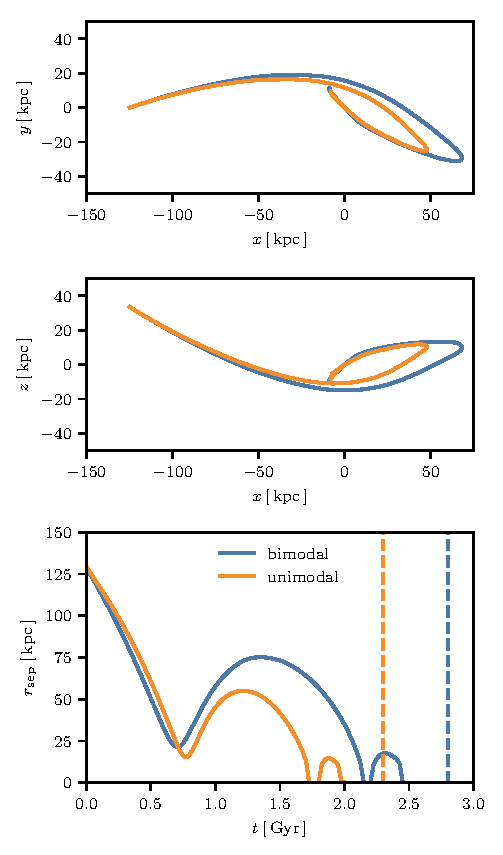
\includegraphics[width=208.14452628pt]{ch3/orbit.pdf}
    \caption{The orbits of the bimodal (blue) and unimodal (orange) simulations. The upper and middle panels show the orbit in the $x$-$y$ and $x$-$z$ planes, respectively. The bottom panel shows the separation distance as a function of time. The orbit begins retrograde but then radializes after the first pericentric passage. The satellite then coalesces quickly after the second pericentric passage, after $\sim2\,\Gyr$ of evolution. A blue dashed line is shown for the bimodal simulation at $2.8\,\Gyr$, the time of a star formation gap at $\FeH=0$ (see Figure~\ref{ch3:fig:before_after}). An orange dashed line is shown for the unimodal simulation (which has no gap) at the same time after its second pericentric passage ($2.3\,\Gyr$).}
    \label{ch3:fig:orbit}
\end{figure}

We used the fiducial halos in \citet{2021ApJ...923...92N} as a starting point for each galaxy. We then manually varied the different model parameters until we arrived at a setup that resulted in reasonable galaxies as determined by their stellar mass. For the central (Milky Way) galaxy, we set $M_{200}=5\times10^{11}\,\Msun$, $c_{200}=4.1$, $\beta=0.8$, $r_c=9\,\kpc$, $f_b=0.08$, and $v_{\phi}/v_{\textrm{c}}=0.2$, where $c_{200}$ is the concentration and $v_{\phi}/v_{\textrm{c}}$ is the azimuthal velocity of the gaseous halo as a fraction of the local circular velocity. For the satellite (GSE) galaxy, we set $M_{200}=2.2\times10^{11}\,\Msun$, $c_{200}=4.33$, $\beta=0.8$, $r_c=6.5\,\kpc$, $f_b=0.06$, and $v_{\phi}/v_{\textrm{c}}=0.4$.

We used a mass resolution of $6\times10^4\,\Msun$ for the gas and $3\times10^5\,\Msun$ for the dark matter. This is closest to a level~4 resolution in the AURIGA simulations \citep{2017MNRAS.467..179G}, and is about $0.7\times$ the mass resolution of TNG50-1 \citep{2019MNRAS.490.3234N,2019MNRAS.490.3196P}. All collisionless particles have a fixed softening length of $40\,\pc$. The gas has a softening length $2.5\times$ the cell size, with a minimum size of $10\,\pc$. Snapshots were saved at intervals of $25\,\Myr$.

The stellar mass build-up of our Milky Way-like and GSE-like galaxies is given in Figure~\ref{ch3:fig:mass_size}. The upper panel shows the stellar mass history. We attempt to match the expected mass of the present-day thick disk \citep[$\sim6\times10^9\,\Msun$, horizontal blue dashed line][]{2016ARA&A..54..529B} at an evolution time of $\sim3\,\Gyr$ (corresponding to $z\sim2$, vertical dashed gray line).\footnote{Of course, this neglects the significant mass contribution of the bulge, which presumably formed earlier. However, our setup does not form a strong spheroidal component. Using the trick in e.g. \citet{2022MNRAS.515.1524Z}, we take the bulge mass to be twice the counter-rotating stellar mass. At $3\,\Gyr$ in the isolated Milky Way-like galaxy, the bulge mass is $\sim7\times10^{8}\,\Msun$, or $\sim13\%$ of the total mass. The Milky Way's bulge is  $\sim1.5\times10^{10}\,\Msun$, although there is strong debate about just how much of the bulge is a classical bulge which formed before the disk \citep{2016ARA&A..54..529B}. In any case, we did not attempt to match any particular property of the bulge, though one could promote bulge formation by reducing the rotation of the gas in the inner region.} We get reasonably close at $\sim5\times10^9\,\Msun$ (blue line). For GSE, we use the best-fit mass from the $N$-body simulations of \citet{2021ApJ...923...92N} -- $5\times10^8\,\Msun$ (horizontal dashed orange line). For this, we slightly overestimate at $\sim6\times10^8\,\Msun$ (orange line).

As for the galaxy sizes, there is significant spread amongst the real galaxy population, and the sizes are thought to be influenced by the merger history not present in our setup \citep[e.g.][]{2014ApJ...788...28V}. We note that the sizes of each simulated galaxy (lower panel) are within the range of observed galaxy sizes. For the Milky Way, we know the thick disk has scale length of $\sim2\,\kpc$, which converts to a half-mass radius of $\sim3.36\,\kpc$. At $\sim3\,\Gyr$, our Milky Way-like galaxy has a half-mass radius of $\sim2\,\kpc$. Curiously, after $3\,\Gyr$, the size of the Milky Way-like galaxy continues to grow while the GSE galaxy's size remains constant for the duration of the simulation.

\subsection{Orbital Configuration}\label{ch3:ssec:orbit_setup}
In order to combine the galaxies, we follow \citet{2021ApJ...923...92N}, and place the satellite on a retrograde orbit. In the fiducial simulation of \citet{2021ApJ...923...92N}, the satellite is placed at the virial radius ($R_0=129\,\kpc$), with the virial velocity ($V_0=129\,\kms$), and with a circularity of $\eta=0.5$. To test minor changes to the orbit, we ran a grid of simulations with $\pm10\%$ in each the starting radius and velocity, and $\pm0.1$ in the circularity, for a total of $27$ simulations. We performed each simulation for a duration of $8\,\Gyr$, and used \texttt{FOF} and \texttt{SUBFIND} in order to identify substructure \citep{2005Natur.435..629S,2009MNRAS.399..497D}.

Some of the simulations in this orbital grid resulted in bimodal abundance distributions, while some had little to no structure in the abundance distribution plane. We will first study two representative simulations in detail chosen based on their structure in the abundance plane as shown in Figure~\ref{ch3:fig:fig1}, one which we refer to as bimodal and one as unimodal. For the bimodal simulation, we chose the simulation with $R_0=129\,\kpc$, $V_0=142\,\kms$, and $\eta=0.4$. For the unimodal simulation, the parameters are the same except that $V_0=116\,\kms$. These simulations will later be identified as having the highest and second lowest bimodality score $\mathcal{B}$. We will then examine the full simulation suite, and show the detailed abundance plane for the full suite in Appendix~\ref{ch3:app:allmerge}.

We show the bimodal and unimodal simulations' orbits in Figure~\ref{ch3:fig:orbit}. We use a shrinking spheres center of mass method to identify the centers of the central and satellite galaxy \citep[e.g.,][]{2003MNRAS.338...14P}.\footnote{The position of the minimum potential particle in each substructure identified by \texttt{SUBFIND} is used as the starting guess, and we use an initial/final radius and step factor of $10\,\kpc$, $5\,\kpc$, and $0.9$, respectively.} The upper and middle panels show the orbits in the $x$-$y$ and $x$-$z$ planes, respectively. The lower panel shows the separation distance as a function of time. The orbit is initially retrograde, but quickly radializes after the first pericentric passage. Coalescence occurs rapidly after the second pericentric passage at $\sim2\,\Gyr$, and \texttt{SUBFIND} ceases to recognize the satellite as a separate subhalo.

\subsection{Feedback and Enrichment Model}\label{ch3:ssec:gfm}
Our feedback model is a variant of the Illustris TNG model \citep{2013MNRAS.436.3031V,2017MNRAS.465.3291W,2018MNRAS.473.4077P}. In this model, gravity and magnetohydrodynamics are solved using a \citet{1986Natur.324..446B} tree coupled to a second order finite volume fluid solver in AREPO \citep{2010MNRAS.401..791S,2016MNRAS.455.1134P}. Stellar feedback is included through a subgrid wind particle model \citep{2003MNRAS.339..289S}. AGN feedback follows a dual kinetic and thermal mode for low- and high-accretion rates \citep{2017MNRAS.465.3291W}, though in our setup the AGN is only ever in the high-accretion mode. The central galaxy is seeded with a black hole with the typical seed mass ($8\times10^5\,\Msun$). 

In this work, we made some simplifications to this model in order to aid interpretation. First, we ignore magnetic fields. This was motivated by an initial desire to understand the CGM accretion rates in terms of idealized cooling flow solutions, but we did not revisit turning them back on. In any case, it is not clear if the magnetic fields would be realistically generated given our initial setup. Second, we use a gentler wind feedback model as described in \citet{2019MNRAS.489.4233M}. Because our setup includes both an initially steep central potential and no steady-state disk, a stronger feedback model would require a higher central gas density to achieve a reasonable SFH which introduced its own set of pathological instabilities.

In this model, star particles synthesize elements through three different channels for which we cite the relevant yield tables: SNe Ia \citep{1997NuPhA.621..467N}, SNe II \citep{1998A&A...334..505P,2006ApJ...653.1145K}, and AGB stars \citep{2010MNRAS.403.1413K,2014MNRAS.437..195D,2014ApJ...797...44F}. Each star particle, which is modeled as a simple stellar population, continuously injects metals into its surroundings in the following sequence\footnote{The kinetic/thermal feedback component is handled through the wind generation, which is completely separate in this model.}:
\begin{enumerate}
    \item $t\lesssim10\,\Myr$: no metal injection as the first supernova ($M\sim100\,\Msun$) has not gone off
    \item $10\,\Myr \lesssim t \lesssim 40\,\Myr$: metal injection as $8\,\Msun<M<100\,\Msun$ stars die as Type II SNe
    \item $t\gtrsim40\,\Myr$: metal injection from Type Ia SNe and AGB stars
\end{enumerate}
There are a few things to note about this model: (1) The exact timings are metallicity-dependent. (2) The \MgFe{} of ejected gas from Type II SNe is mass/time-dependent, with more massive stars contributing more Mg than less massive stars. (3) In a Hubble time, type II SNe contribute the vast majority of Mg ($\sim10\times$ AGB and $\sim100\times$ Type Ia SNe). Type Ia and Type II SNe contribute approximately equal amounts of Fe (each $\sim3\times$ AGB). See Figure~1 from \citet{2018MNRAS.473.4077P}. (4) The number of Type Ia SNe is greater for a younger stellar population, with a power law relationship $\propto \left(t/\tau_8\right)^{-1.12}$, where $\tau_8=40\,\Myr$ is the lifetime of an $8\,\Msun$ star.

\subsection{Observed Abundances}\label{ch3:ssec:obs_abund}
Our aim in this work is to demonstrate the feasibility of a mechanism for structure formation in the abundance plane. We are only making a qualitative comparison to data. Therefore, we use the ASPCAP DR17 catalog of stellar abundances \citep[][J.A.~Holtzman et al., in preparation]{2016AJ....151..144G}, which is publicly available, well-established, and widely used.

We applied quality cuts and restricted our sample to giants, requiring:
\begin{itemize}[noitemsep]
    \item $\textrm{SNR} > 200$,
    \item $\textrm{VSCATTER} < 1\,\kms$,
    \item $\textrm{STARFLAG not set}$,
    \item $\varpi/\sigma_{\varpi} > 1$,
    \item $\log{g} < 3.5$,
    \item $\sigma_{\log{g}} < 0.2$,
\end{itemize}
where $\varpi$ is the parallax. We use the parallax, proper motion, and radial velocity from Gaia EDR3 \citep{2016A&A...595A...1G,2021A&A...649A...1G,2021A&A...649A...2L,2021A&A...653A.160S}.

We next make a solar neighborhood selection of stars based on their angular momenta. We assume the solar radius and azimuthal velocity are $R_0=8\,\kpc$ and $V_0=220\,\kms$ \citep{2016ARA&A..54..529B}, and select stars which have $L_z$ within $10\%$ of the solar angular momentum. We further require that $\left|z\right| < 3\,\kpc$. As is typically done, we use \FeH{} as an indicator of the total metallicity of a star. We use Mg alone as a representative of the $\alpha$-elements.

For stellar ages, we used the APOKASC-3 catalog \citep{2025ApJS..276...69P}. This catalog uses a combination of APOGEE spectroscopic parameters and \textit{Kepler} time series photometry to compute astroseismic ages. Using only stars with $25\%$ age uncertainties (taken as the maximum of the upper and lower uncertainty), we cross-match this catalog to our larger sample from ASPCAP which results in a sample of 2525 stars.

\subsection{Solar Neighborhood in Simulations}\label{ch3:ssec:solarneigh}
When comparing galaxy simulations to the observed solar neighborhood, some ambiguity arises in how to make a ``solar neighborhood-like'' selection of star particles. Naturally, this selection is dependent on the posed question, which in this work is the formation of the abundance bimodality. The Sun is known to sit near the end of the thick disk, where the thick and thin disk have comparable surface densities \citep[the ratio of thick-to-thin is $\sim12\%$][]{2016ARA&A..54..529B}. As a result, the abundance bimodality appears most strongly near the Sun -- further inwards the high-$\alpha$ sequence is more dominant and further outwards the high-$\alpha$ sequence vanishes \citep[e.g.,][]{2015ApJ...808..132H}.

We mimic our selection of the solar neighborhood by also making a cut in angular momentum. However, in the simulation, the high-$\alpha$ disk is more compact than in the Galaxy. Therefore, in order to strike a balance between the low-$\alpha$ and high-$\alpha$ disks, we used an angular momentum cut which is $20\%$ that of our assumed solar angular momentum. In particular, we select all star particles with angular momenta within $30\%$ of $0.2\times8\,\kpc\times220\,\kms$ -- as well as requiring $\left| z \right| < 3\,\kpc$. This corresponds to roughly selecting star particles with radii between $2$ and $5\,\kpc$.

\subsection{Bimodality Score}\label{ch3:ssec:bim_score}
Given the modest size of our suite, some method for scoring the degree of bimodality for a given 1D distribution is desirable. Tests of whether a distribution is bimodal or unimodal exist -- e.g., the Hartigan dip test \citep{10.1214/aos/1176346577}, but they lack the ability to rank order based on ``bimodalitiness.'' In order to do this, we fit a given distribution of \alphaFe{} as a two-component Gaussian mixture model. The bimodality score $\mathcal{B}$ is then computed as
\begin{equation}\label{eq:bimscore}
\mathcal{B} = \frac{\left|\mu_1-\mu_2\right|}{\sqrt{\sigma_1^2-\sigma_2^2}}\times w(A_2, t, k)\textrm{,}
\end{equation}
where $(\mu_1, \sigma_1)$ is the mean and standard deviation of the higher weighted mode, $(\mu_2, \sigma_2)$ likewise for the less weighted mode, $A_2$ is the amplitude of the less weighted mode, and $w$ is a penalty function with parameters $t$ and $k$ given by
\begin{equation}\label{eq:bimscore_penalty}
w(A, t, k) = \left[1+e^{-k\left(A-t\right)}\right]^{-1}\text{.}
\end{equation}
We take $t$ and $k$ to be $0.1$ and $20$, respectively.

This metric effectively measures the distance between two modes normalized by their variances, with a penalty when one mode is not highly weighted. These choices were made in order for the score to match by eye which distributions appear to have one as opposed to two peaks, and was found to empirically be more reliable than other statistics like peak-to-trough ratios or mode overlap. As demonstrated in Section~\ref{ch3:ssec:full_sim_suite}, a score of $\mathcal{B}>2.25$ appears to select the bimodal populations.

\section{Results}\label{ch3:sec:results}
\subsection{Surface Density Projections}\label{ch3:ssec:projections}
Before dissecting the simulated galaxies in detail, we first examine the surface density projections of the gas and stars in the central region, situated on the central galaxy in the bimodal simulation. This is shown in Figure~\ref{ch3:fig:projections}. In each grouping of four, the bottom and top rows show the face-on and edge-on views, respectively. The left and right columns show the gas (blue) and stellar (orange) surface density, respectively. Each panel is oriented with respect to the stellar angular momentum of the final snapshot ($t=8\,\Gyr$), computed using all star particles within the half-mass radius.

We can see that the galaxy grows in size after the merger. Additionally, the galaxy's orientation continues to change even within the last $3\,\Gyr$. The final galaxy is oriented $\sim126\degree$ with respect to the initial orientation of the central galaxy's gas halo. The dynamical and kinematic consequences of such a gas-rich merger is beyond the scope of our current work.

% \begin{figure*}
%   \centering

%     \gridline{\fig{ch3/bimodal_L30_frame60.pdf}{132.254238pt}{}
%               \fig{ch3/bimodal_L30_frame70.pdf}{132.254238pt}{}
%               \fig{ch3/bimodal_L30_frame80.pdf}{132.254238pt}{}
%               }
%     \gridline{\fig{ch3/bimodal_L30_frame90.pdf}{132.254238pt}{}
%               \fig{ch3/bimodal_L30_frame100.pdf}{132.254238pt}{}
%               \fig{ch3/bimodal_L30_frame110.pdf}{132.254238pt}{}
%               }
%     \gridline{\fig{ch3/bimodal_L30_frame120.pdf}{132.254238pt}{}
%               \fig{ch3/bimodal_L30_frame200.pdf}{132.254238pt}{}
%               \fig{ch3/bimodal_L30_frame320.pdf}{132.254238pt}{}
%               }
%   \caption{Frames from a movie showing a surface density projection of the bimodal simulation over time. In each frame, the left/right (blue/orange) column shows the gas/star surface density. The upper/lower panels show the edge-on and face-on view. Every panel is oriented with respect to the final ($t=8\,\Gyr$) snapshot. The side-length of each panel is $30\,\kpc$, and the image is a projection through a box with the same side-length. The color map for the gas ranges from $1$ to $10^2\,\Msun/\pc^2$, while for the stars ranges from $1$ to $10^4\,\Msun/\pc^2$. Description of movie: The disk collapses quickly, forming a disk within $500\,\Myr$. The satellite galaxy quickly passes in the background at $\sim700\,\Myr$. At $\sim2\,\Gyr$, the satellite directly merges with the central galaxy, fully coalescing by $\sim3\,\Gyr$. Over the next $5\,\Gyr$, the disk steadily grows, expanding in size. (A full movie is available in published version.)}
%   \label{ch3:fig:projections}
% \end{figure*}

\begin{figure*}
    \centering
    % First row of images
    \begin{minipage}{132.254238pt}
        \centering
        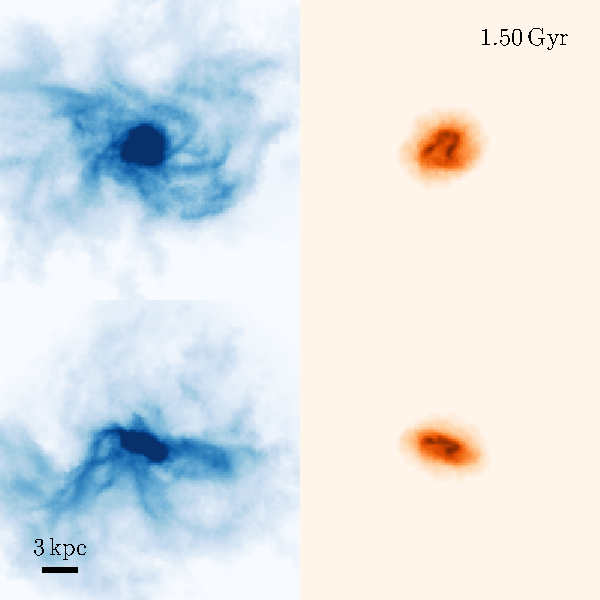
\includegraphics[width=132.254238pt]{ch3/bimodal_L30_frame60.pdf}
    \end{minipage}
    \begin{minipage}{132.254238pt}
        \centering
        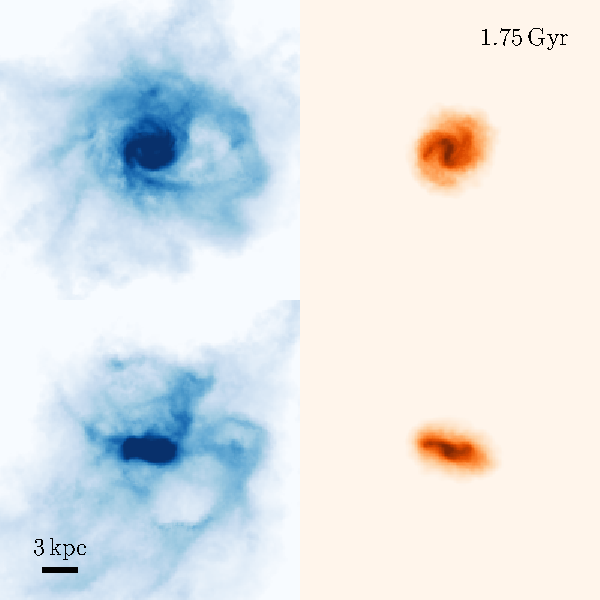
\includegraphics[width=132.254238pt]{ch3/bimodal_L30_frame70.pdf}
    \end{minipage}
    \begin{minipage}{132.254238pt}
        \centering
        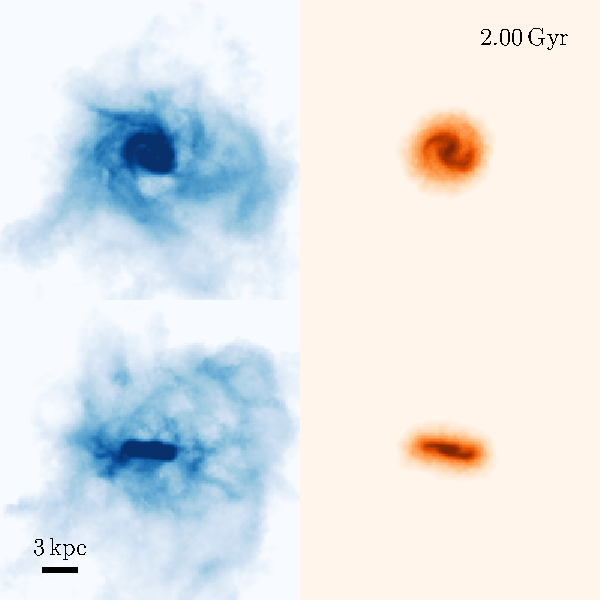
\includegraphics[width=132.254238pt]{ch3/bimodal_L30_frame80.pdf}
    \end{minipage}

    % Second row of images
    \vspace{1mm}  % Adjust spacing between rows if needed
    \begin{minipage}{132.254238pt}
        \centering
        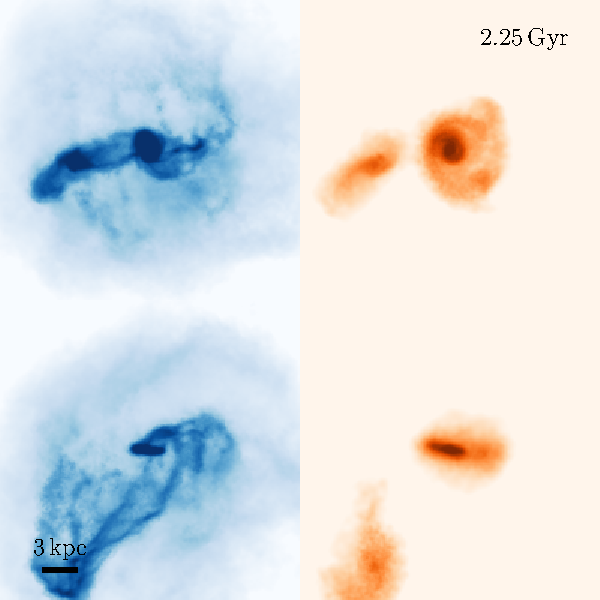
\includegraphics[width=132.254238pt]{ch3/bimodal_L30_frame90.pdf}
    \end{minipage}
    \begin{minipage}{132.254238pt}
        \centering
        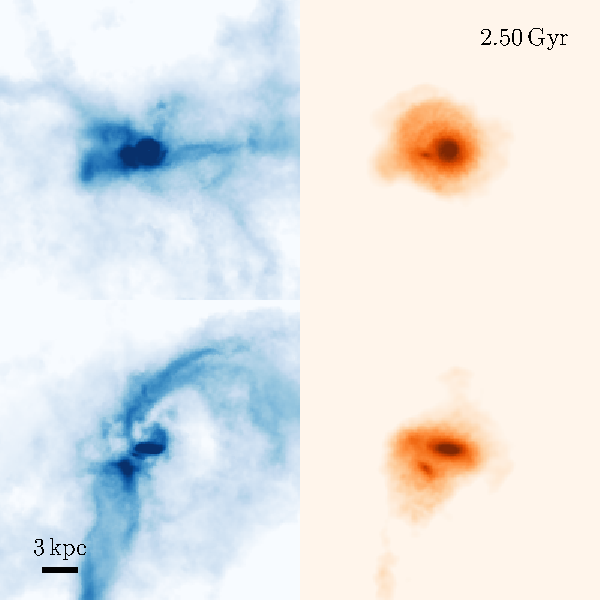
\includegraphics[width=132.254238pt]{ch3/bimodal_L30_frame100.pdf}
    \end{minipage}
    \begin{minipage}{132.254238pt}
        \centering
        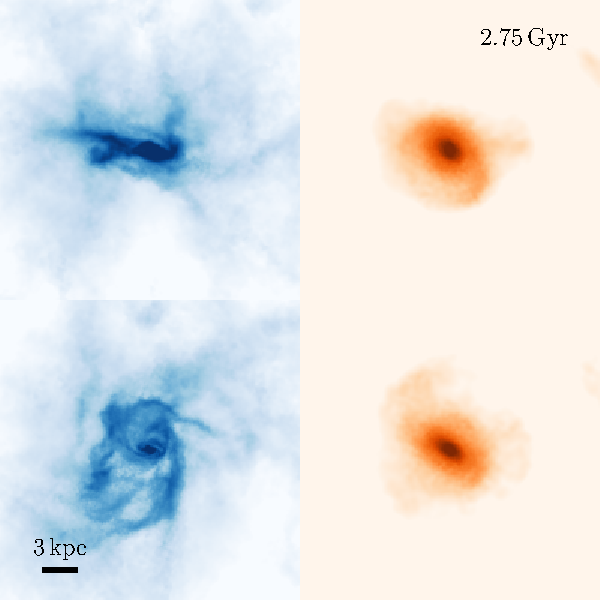
\includegraphics[width=132.254238pt]{ch3/bimodal_L30_frame110.pdf}
    \end{minipage}

    % Third row of images
    \vspace{1mm}
    \begin{minipage}{132.254238pt}
        \centering
        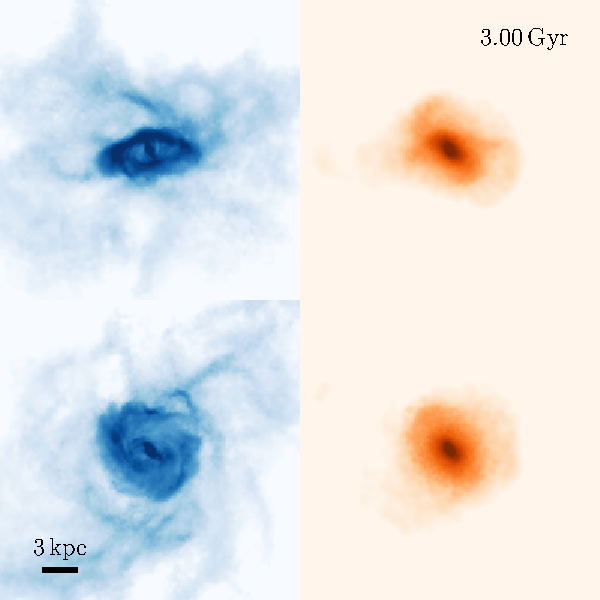
\includegraphics[width=132.254238pt]{ch3/bimodal_L30_frame120.pdf}
    \end{minipage}
    \begin{minipage}{132.254238pt}
        \centering
        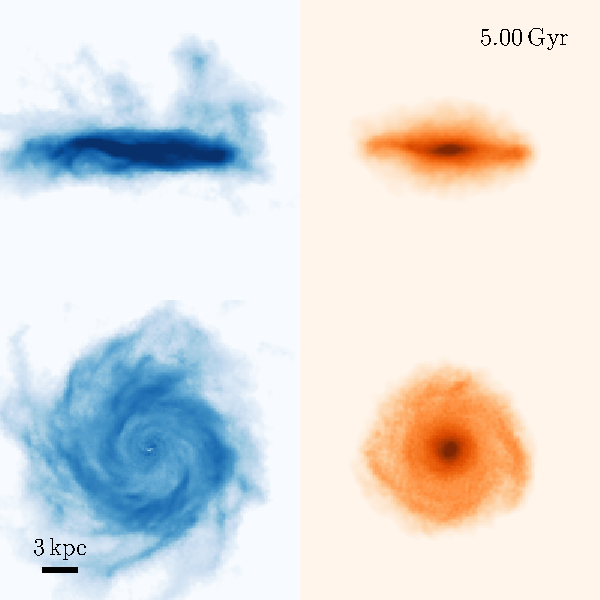
\includegraphics[width=132.254238pt]{ch3/bimodal_L30_frame200.pdf}
    \end{minipage}
    \begin{minipage}{132.254238pt}
        \centering
        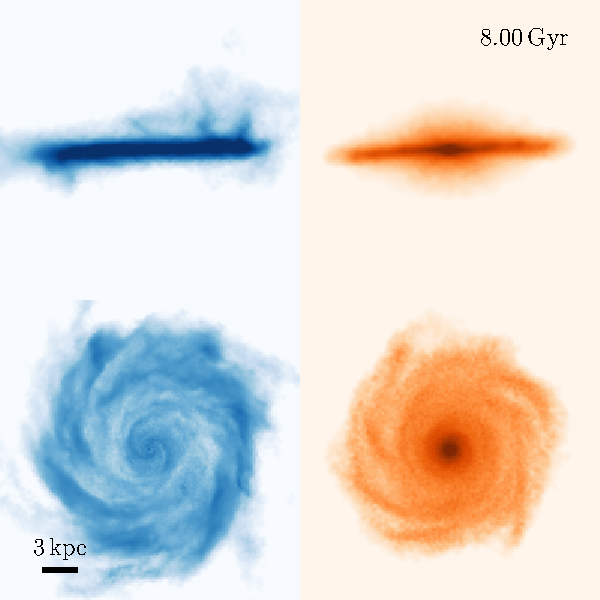
\includegraphics[width=132.254238pt]{ch3/bimodal_L30_frame320.pdf}
    \end{minipage}

    % Caption
    \caption{Frames from a movie showing a surface density projection of the bimodal simulation over time. In each frame, the left/right (blue/orange) column shows the gas/star surface density. The upper/lower panels show the edge-on and face-on view. Every panel is oriented with respect to the final ($t=8\,\Gyr$) snapshot. The side-length of each panel is $30\,\kpc$, and the image is a projection through a box with the same side-length. The color map for the gas ranges from $1$ to $10^2\,\Msun/\pc^2$, while for the stars ranges from $1$ to $10^4\,\Msun/\pc^2$. Description of movie: The disk collapses quickly, forming a disk within $500\,\Myr$. The satellite galaxy quickly passes in the background at $\sim700\,\Myr$. At $\sim2\,\Gyr$, the satellite directly merges with the central galaxy, fully coalescing by $\sim3\,\Gyr$. Over the next $5\,\Gyr$, the disk steadily grows, expanding in size. (A full movie is available in the published version.)}
    \label{ch3:fig:projections}
\end{figure*}

\subsection{Abundance Distribution}\label{ch3:ssec:abundplane}
\begin{figure*}
  \centering
  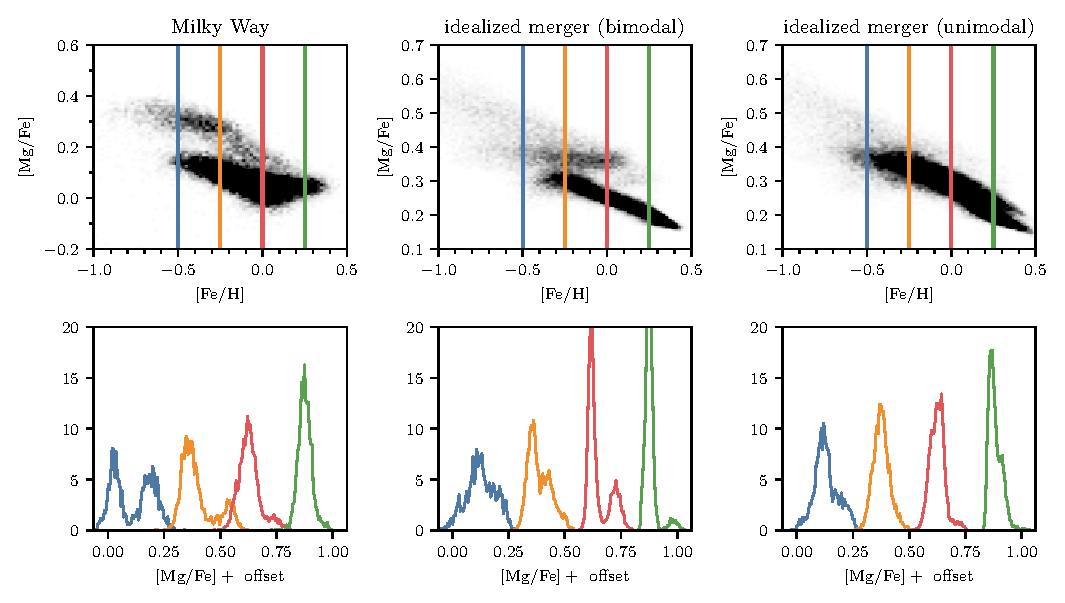
\includegraphics[width=\textwidth]{ch3/figure1.pdf}
  \caption{The abundance bimodality seen in the Milky Way can be reproduced in some idealized merger simulations. In the upper panels, we show the distribution of stars in the \MgFe{}-\FeH{} plane. The lower panels show the distribution of \MgFe{} at a fixed \FeH{} bin of width $0.05\,\dex$. The colors indicate the fixed \FeH values, which are $-0.5$, $-0.25$, $0$, and $0.25$. The left column shows the observed distribution in the Milky Way from ASPCAP DR17 \citep[][J.A.~Holtzman et al., in preparation]{2016AJ....151..144G}, while the right two columns show two idealized merger simulations. The idealized merger simulations are nearly identical, except that in the bimodal simulation the satellite has a starting velocity of $142\,\kms$, while in the unimodal simulation it has a starting velocity of $116\,\kms$. The labels ``unimodal'' and ``bimodal'' are of the \textit{outcome} of the simulation, and do not reflect a particular choice in the setup. The Milky Way (left column) exhibits a strong bimodal distribution of \MgFe{} at various \FeH{}. The idealized merger simulation marked as bimodal (center column) also exhibits a bimodal distribution of \MgFe{}, though the structure is not as strongly defined. The idealized merger simulation marked as unimodal (right column) exhibits only weak structure, if any at all.}
  \label{ch3:fig:fig1}
\end{figure*}

In Figure~\ref{ch3:fig:fig1}, we show the abundance distribution of the Milky Way as well as two of our idealized merger simulations in the upper panels. A number of our idealized simulations exhibit either a bimodal or unimodal abundance distribution, and so we have selected two representative examples as discussed in Section~\ref{ch3:ssec:orbit_setup}. The bimodal and unimodal labels are of the outcome of the simulation, and do not reflect any particular choice made in their setup.

There are, of course, differences between the bimodal simulation and the Milky Way. First, the scaling in \MgFe{} is different -- in the simulation, the low-$\alpha$ sequence lies at $\sim0.2$, while in the Milky Way it is at about $\MgFe\sim0$. Second, in the Milky Way the high-$\alpha$ sequence neatly joins the low-$\alpha$ sequence at $\FeH\sim0$, while in the simulation the two actually diverge more at higher \FeH{}.

In the lower panels of Figure~\ref{ch3:fig:fig1}, we show the distributions of \MgFe{} at different fixed \FeH{}. The (blue, orange, red, green) lines show the \MgFe{} distribution at a \FeH{} of ($-0.5$, $-0.25$, $0$, $0.25$), in bins of width $0.05\,\dex$. The distributions of \MgFe{} are offset (but not rescaled) so that they do not overlap. Here, the bimodality seen in the Milky Way is quite striking at lower metallicities. The peaks are well-separated, by $\sim0.2\,\dex$. In the bimodal simulation, the distribution is still clearly bimodal, but the peaks are less well-separated, by $\sim0.1\,\dex$. In the unimodal simulation, there is a hint of some structure at $\FeH > 0.25$, but there is not a strong multimodal structure.

\subsection{Build up of the Abundance Plane}\label{ch3:ssec:abundplane_build}
Next, we examine the build up of the abundance plane. In the left panel of Figure~\ref{ch3:fig:before_after}, we show the metallicity-dependent star formation rate of the bimodal simulation using star particles in the solar neighborhood at the end of the simulation within a $0.1\,\dex$ bin centered at $\FeH=0$. There is a clear dip in the SFR at $\sim2.8\,\Gyr$, which we indicate with a vertical line.

In the center left panel, we show the abundance plane distribution from the bimodal simulation for all stars in the solar neighborhood, replicating Figure~\ref{ch3:fig:fig1}. A dashed line at $-0.1\times\FeH+0.3$, chosen by eye, is plotted to demarcate the high- and low-$\alpha$ sequences. In the center right and right panels, we show the distribution of star particles which form before and after the dip in the metallicity-dependent SFR at $t=2.8\,\Gyr$, respectively. The vast majority of the high-$\alpha$ sequence forms before the dip, while most of the low-$\alpha$ sequence forms afterward.

This sequence of build up is markedly different in the unimodal simulation, which we show in Figure~\ref{ch3:fig:before_after_uni}. Here, there is no clear dip in the metallicity dependent SFR in the left panel. We still place a vertical line similar to the one in Figure~\ref{ch3:fig:before_after}, except now it is chosen to be at $t=2.3\,\Gyr$, which is $\sim300\,\Myr$ after the second pericentric passage. This is where the gap appears in the bimodal simulation (see Figure~\ref{ch3:fig:orbit}). We see that stars which form before and after this point in the simulation overlap considerably in the abundance plane.

The timing and duration of the metallicity-dependent SFR dip is not the same for all \FeH{}. In the upper panel of Figure~\ref{ch3:fig:before_after_sfh_by_iron}, we show the SFR at metallicities of $-0.5$, $-0.25$, $0$, and $0.25$ in blue, orange, red, and green, respectively. We mark the location of the dip in the red $\FeH=0$ SFR with a vertical line at $t=2.8\,\Gyr$, as in Figure~\ref{ch3:fig:before_after}. In the orange SFR at $\FeH=-0.25$, which displayed a prominent bimodality in Figure~\ref{ch3:fig:fig1}, there is a similar dip. However, it occurs about $250\,\Myr$ earlier. The $\FeH=0$ and $\FeH=-0.25$ dips have widths of about $500$ and $250\,\Myr$, respectively. In the blue $\FeH=-0.25$ SFR, which does not display a prominent bimodality, there is no dip separating two periods of sustained SF. In the green $\FeH=0.25$ SFR, a small amount of SF occurs before an extended $\sim1\,\Gyr$ dip, leading to a bimodality with a weak although well-separated high-$\alpha$ mode.

In the lower panel of Figure~\ref{ch3:fig:before_after_sfh_by_iron}, we show corresponding curves for the unimodal simulation. A vertical line is shown at $2.3\,\Gyr$, as described earlier. Here, we see that at no \FeH{} is there a prominent dip.

\begin{figure*}
  \centering
  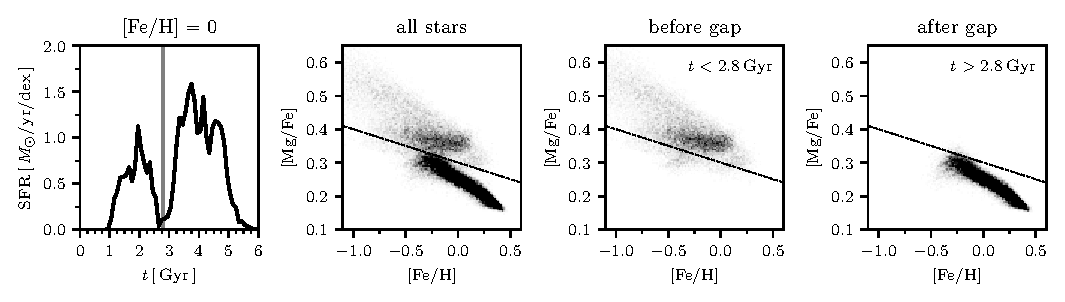
\includegraphics[width=\textwidth]{ch3/before_after.pdf}
  \caption{The buildup of the abundance plane in the bimodal simulation. The left panel shows the metallicity-dependent star formation rate (SFR) for star particles in the solar neighborhood at the end of the simulation, selected within a $0.1\,\dex$ bin centered at $\FeH=0$. A clear dip in this SFR occurs at $t \sim 2.8\,\Gyr$, marked by the vertical line. The center-left panel shows the abundance plane distribution for all stars in the solar neighborhood, with a dashed line at $-0.1\times\FeH+0.3$ (chosen by eye) demarcating the high- and low-$\alpha$ sequences. The center-right and right panels show the abundance plane distributions for stars formed before and after the SFR dip, respectively. The majority of the high-$\alpha$ sequence forms before the dip, while most of the low-$\alpha$ sequence forms afterward.}
  \label{ch3:fig:before_after}
\end{figure*}

\begin{figure*}
  \centering
  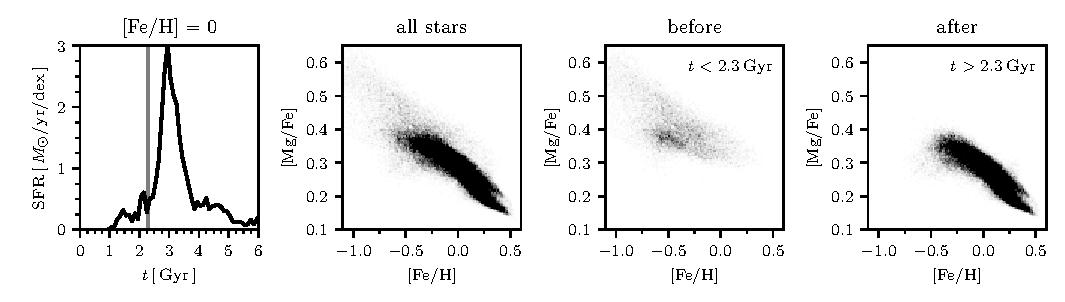
\includegraphics[width=\textwidth]{ch3/before_after_uni.pdf}
  \caption{The buildup of the abundance plane in the unimodal simulation, similar to Figure~\ref{ch3:fig:before_after}. The left panel shows the metallicity-dependent star formation rate (SFR) for stars in the solar neighborhood, with no clear dip. A vertical line at $t=2.3\,\Gyr$, corresponding to the orbital stage of the gap in the bimodal simulation (see text), is included for comparison. The center left shows the abundance plane for all stars. The center-right and right panels show the abundance plane for stars formed before and after $t=2.3\,\Gyr$, respectively. Unlike the bimodal case, stars formed before and after this time overlap considerably in the abundance plane, indicating the absence of a distinct separation between high- and low-$\alpha$ sequences.}
  \label{ch3:fig:before_after_uni}
\end{figure*}

\begin{figure}
  \centering
  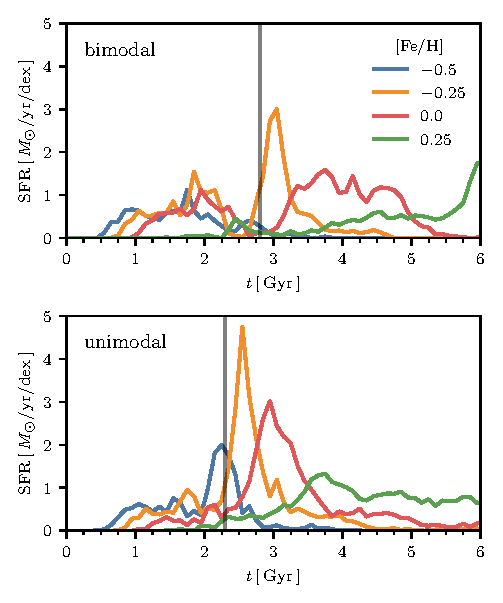
\includegraphics[width=208.14452628pt]{ch3/before_after_sfh_by_iron.pdf}
  \caption{Metallicity-dependent star formation histories (SFH) for the bimodal (top) and unimodal (bottom) simulations. The SFH at different metallicities ($\FeH=-0.5, -0.25, 0.0, 0.25$) is shown in blue, orange, red, and green, respectively. In the top panel, the vertical line at $t=2.8\,\Gyr$ marks the SFR dip at $\FeH=0$, corresponding to the gap seen in Figure~\ref{ch3:fig:before_after}. A similar dip is present in the orange $\FeH=-0.25$ SFR, but it occurs $\sim250\,\Myr$ earlier, with a width of about $250\,\Myr$. The $\FeH=-0.5$ (blue) SFR lacks a distinct dip, while the $\FeH=0.25$ (green) SFR features an extended $\sim1\,\Gyr$ dip after a short period of SF, leading to a weak but well-separated high-$\alpha$ mode. The bottom panel shows the corresponding SFHs for the unimodal simulation, with a vertical line at $t=2.3\,\Gyr$. There are no strong dips at any metallicity, consistent with the absence of a well-defined bimodality.}
  \label{ch3:fig:before_after_sfh_by_iron}
\end{figure}

\begin{figure*}
  \centering
  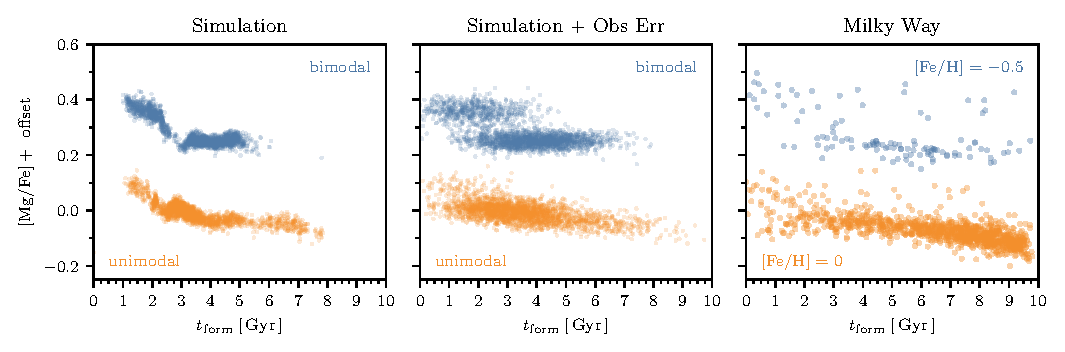
\includegraphics[width=\textwidth]{ch3/alpha_vs_tform_obserr.pdf}
  \caption{In the bimodal simulation, a gap appears when plotting stars in a $0.05\,\dex$ bin at $\FeH=0$ on the \MgFe{}-$t_{\textrm{form}}$ plane (blue, left panel). In the unimodal simulation there is no such gap (orange, left panel). In the middle panel, we show the same data but assuming errors in \FeH{}, \MgFe{}, and $t_{\textrm{form}}$ of $0.0075\,\dex$, $0.012\,\dex$, and $1\,\Gyr$, respectively. The gap in the bimodal simulation appears weakly as two populations overlapping in age. In the right panel we show stars in the Milky Way from APOKASC3 in $0.2\,\dex$ bins at $\FeH=-0.5$ (blue) and $0$ (orange). The low-metallicity bin is where the Milky Way bimodality is strongest while there is no bimodality at the solar-metallicity bin (see Figure~\ref{ch3:fig:fig1}). Offsets have been added to \MgFe{} values for clarity: $-0.3$ in the unimodal points in the left and middle panels, and $+0.1$ and $-0.1$ in the low/solar-metallicity bins, respectively, in the right panel.}
  \label{ch3:fig:alpha_vs_tform}
\end{figure*}

\subsection{Comparison to Observations}\label{ch3:ssec:compare_obs}
A plot of \MgFe{} vs age or formation time is a useful way to further demonstrate the formation scenario of the bimodality, as well as making comparison to observations. We show this for the simulation data in the left panel of Figure~\ref{ch3:fig:alpha_vs_tform} in bins of width $0.05\,\dex$ centered at $\FeH=0$. The bimodal simulation (blue, upper data) displays a gap in the ages at $\sim2.8\,\Gyr$, coinciding with the gap in Figure~\ref{ch3:fig:before_after}. On the other hand, the unimodal simulation (orange, lower data) displays no such age gap.

The center panel shows these simulation data points convolved with realistic observational errors. We assume errors in \FeH{}, \MgFe{}, and $t_{\textrm{form}}$ of $0.0075\,\dex$, $0.012\,\dex$, and $1\,\Gyr$, respectively.\footnote{The \FeH{} error impacts which star particles lie in the \FeH{} selection.} The \FeH{} and \MgFe{} errors are characteristic of the errors provided in the APOGEE dataset, and the $1\,\Gyr$ comes from assuming the typical $12.5\%$ uncertainty from APOKASC-3 at an age of $8\,\Gyr$. In the bimodal simulation (blue, upper data), separate populations can be seen that overlap significantly in $t_{\textrm{form}}$. There is not a strong separation in the unimodal case (orange, lower data).

The right panel shows observational data from APOKASC-3. We show in the blue, upper data a $0.2\,\dex$ bin centered at $\FeH=-0.5$ and in the orange, lower data centered at $\FeH=0$. In the Milky Way, there is a bimodal and unimodal \MgFe{} distribution at these metallicities, respectively. At $\FeH=-0.5$, one could weakly argue that there are separate populations as in the simulation. However, the large uncertainties at the relevant ages ($\sim1\,\Gyr$ at ages of $\sim8\,\Gyr$) and the small sample size (125 and 1175 at $\FeH=-0.5$ and $0$, respectively) prevents a definitive statement from being made. Larger sample sizes and more precise age estimates in the future would clarify the connection between simulation and observation, although achieving age uncertainties of $<10\%$ for such old stars is very challenging \citep[e.g.][]{2010ARA&A..48..581S}.

There is an additional complication in the data coming from the presence of young, $\alpha$-rich stars. These have been argued to be old stars with misclassified astroseismic ages due to binary mass transfer \citep[and references therein]{2023A&A...671A..21J}, though with some appearing to be genuinely young \citep[and references therein]{2024arXiv241002962L}, with a range of explanations given \citep[e.g.][]{2015A&A...576L..12C,2021MNRAS.508.4484J,2023arXiv231105815S}. It is unclear which of the $\alpha$-rich stars faithfully reflect the mean ISM chemistry at their inferred age, and so it is not obvious if any detailed conclusions can be drawn from this comparison.

\subsection{Full Simulation Suite}\label{ch3:ssec:full_sim_suite}
We next expand our discussion to the full simulation suite by studying the conditional 1D \MgFe{} distribution in Figure~\ref{ch3:fig:all_hist}. We plot the distribution of \MgFe{} for all stars with \FeH{} lying in a bin of width $0.1\,\dex$ centered at $0\,\dex$. Each distribution corresponds to a choice in the three orbital variables $R_0$, $V_0$, and $\eta$. We rank the simulations in alphabetical order from least to most bimodal\footnote{There is one more simulation in the suite than letters in the English alphabet, so the simulation with the highest bimodality score is labeled aa.}, as determined by the bimodality score $\mathcal{B}$ introduced in Section~\ref{ch3:ssec:bim_score}. The list of simulations in the orbital grid along with the associated orbital parameters and bimodality scores is given in Table~\ref{tab:my-table}.

Simulations from r onward, which have $\mathcal{B}>2.25$, are considered bimodal. This demarcation was chosen by eye using Figure~\ref{ch3:fig:all_hist}. For these simulations, we plot the trough \MgFe{} (the location of the minimum between the two maxima) as a vertical line. This value was determined by taking the location of the minimum of the distribution between $0.25$ and $0.35\,\dex$, and is also given in Table~\ref{tab:my-table}.

Simulations from r to aa have clear bimodalities. The trough \MgFe{} is roughly consistent between simulations, appearing between $\sim0.25$ and $0.3\,\dex$. For simulations marked as unimodal, some appear to have two populations but which are not distinct enough to form a clear bimodality (e.g., m, n, and o).

\begin{figure*}
  \centering
  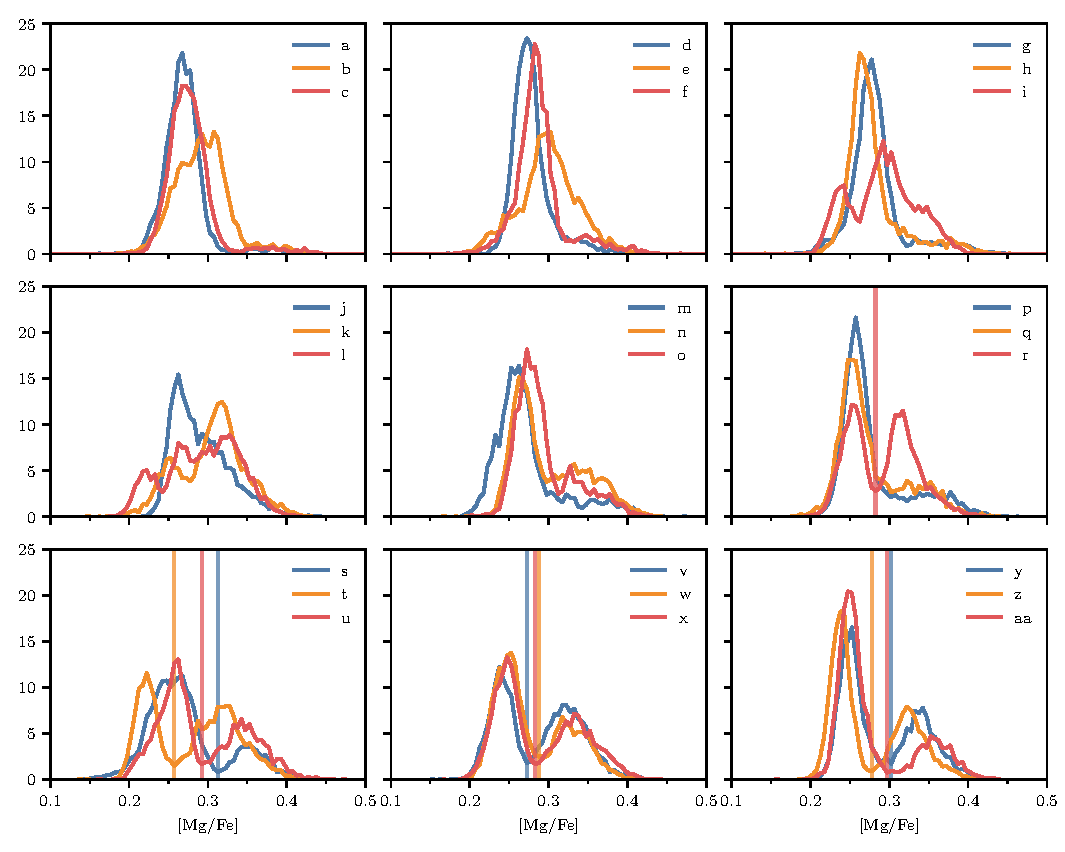
\includegraphics[width=\textwidth]{ch3/hist.pdf}
  \caption{The conditional 1D \MgFe{} distribution for all stars with \FeH{} in a bin of width $0.1\,\dex$ centered at $0\,\dex$. Each panel corresponds to a different set of orbital parameters ($R_0$, $V_0$, and $\eta$) and is labeled alphabetically from least to most bimodal, with the labels defined in Table~\ref{tab:my-table}. The final simulation, which has the highest bimodality score $\mathcal{B}$, is labeled ``aa.'' Simulations with $\mathcal{B}>2.25$ (starting from simulation r) exhibit clear bimodalities, with the trough \MgFe{} (minimum between the two peaks) marked. This trough generally falls between $0.25$ and $0.3\,\dex$. Simulations with lower bimodality scores appear unimodal, though some (e.g., m, n, and o) show hints of a secondary population without forming a distinct bimodal structure.}
  \label{ch3:fig:all_hist}
\end{figure*}

\begin{table}[]
\centering
\begin{tabular}{cccccc}
$\textrm{letter}$ & $R_0$ & $V_0$ & $\eta$ & $\mathcal{B}$ & $\textrm{trough}\,\MgFe{}$ \\ \hline
a                 & $129$ & $129$ & $0.4$  & $0.29$        &                            \\
b                 & $129$ & $116$ & $0.4$  & $0.35$        &                            \\
c                 & $116$ & $116$ & $0.4$  & $0.77$        &                            \\
d                 & $142$ & $116$ & $0.5$  & $0.79$        &                            \\
e                 & $142$ & $129$ & $0.6$  & $0.89$        &                            \\
f                 & $116$ & $129$ & $0.4$  & $1.12$        &                            \\
g                 & $116$ & $116$ & $0.5$  & $1.25$        &                            \\
h                 & $116$ & $142$ & $0.4$  & $1.34$        &                            \\
i                 & $142$ & $142$ & $0.5$  & $1.43$        &                            \\
j                 & $129$ & $142$ & $0.5$  & $1.46$        &                            \\
k                 & $142$ & $129$ & $0.4$  & $1.62$        &                            \\
l                 & $142$ & $142$ & $0.6$  & $1.75$        &                            \\
m                 & $116$ & $129$ & $0.5$  & $1.82$        &                            \\
n                 & $129$ & $129$ & $0.5$  & $1.96$        &                            \\
o                 & $129$ & $116$ & $0.5$  & $2.04$        &                            \\
p                 & $116$ & $116$ & $0.6$  & $2.16$        &                            \\
q                 & $116$ & $129$ & $0.6$  & $2.24$        &                            \\ \hline
r                 & $142$ & $129$ & $0.5$  & $2.26$        & $0.283$                    \\
s                 & $142$ & $116$ & $0.4$  & $2.52$        & $0.313$                    \\
t                 & $116$ & $142$ & $0.6$  & $2.59$        & $0.258$                    \\
u                 & $116$ & $142$ & $0.5$  & $2.62$        & $0.293$                    \\
v                 & $142$ & $116$ & $0.6$  & $2.65$        & $0.273$                    \\
w                 & $129$ & $142$ & $0.6$  & $2.66$        & $0.288$                    \\
x                 & $142$ & $142$ & $0.4$  & $2.70$        & $0.283$                    \\
y                 & $129$ & $116$ & $0.6$  & $2.94$        & $0.303$                    \\
z                 & $129$ & $129$ & $0.6$  & $3.12$        & $0.278$                    \\
aa                & $129$ & $142$ & $0.4$  & $3.34$        & $0.298$                   
\end{tabular}
\caption{All simulations in the orbital grid (as defined by $R_0$, $V_0$, and $\eta$) ordered by their bimodality score $\mathcal{B}$. Each simulation is given an identifying letter. For simulations marked as bimodal ($\mathcal{B}>2.25$), we also list the trough \MgFe{}, or location of the minimum of the \MgFe{} distribution.}
\label{tab:my-table}
\end{table}

We study the formation of the 1D distributions in Figure~\ref{ch3:fig:all_hist} through a scatter plot of \MgFe{} vs formation time of star particles in Figure~\ref{ch3:fig:all_scatter}, similar to Figure~\ref{ch3:fig:alpha_vs_tform}. The order and colors are identical as in Figure~\ref{ch3:fig:all_hist}, and we use the same \FeH{} selection. We only plot a random subsample of 350 stars, and points are plotted with a transparency of $\alpha=0.5$ so that the perceived density is slightly higher in cases of overlap. An offset of $-0.2$ and $-0.4$ are given to the second and third (orange and red) simulations in each panel. For simulations marked as bimodal (r through aa), we also plot a horizontal line at the location of the trough \MgFe{}.

Most of the bimodal simulations (r through aa) have a gap in the distribution at around the time of the merger ($\sim2$-$3\,\Gyr$, depending on the orbital parameters). Before this gap, star formation occurs above the trough while after it occurs below the trough. However, there are two exceptions: simulation~t does not have a full gap (though the density does decrease), and simulation~w is irregular, with star formation simultaneously occurring above and below the trough.

In the unimodal simulations (a through q), there does appear to be gaps (d, f, g, h, and o). However, in these cases, there is not a large amount of star formation occurring before the gap, and so the high-$\alpha$ sequence is underemphasized and does not lead to a significant bimodality.

\begin{figure*}
  \centering
  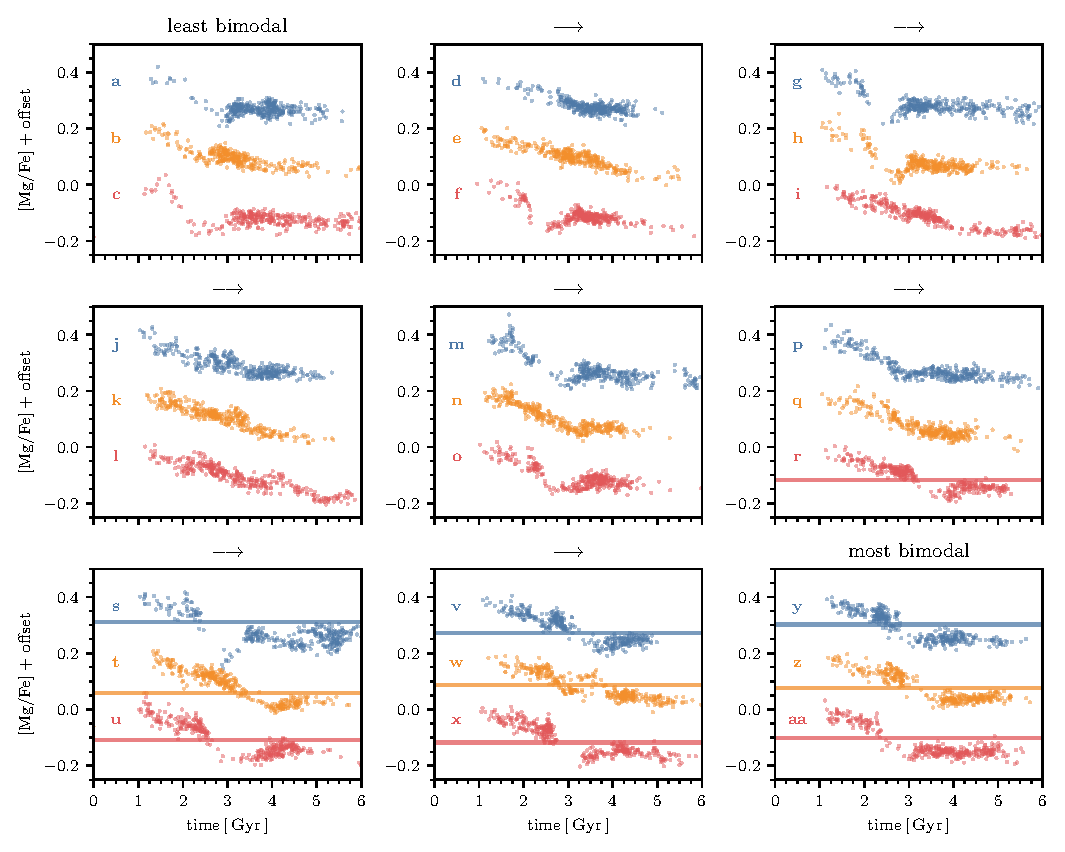
\includegraphics[width=\textwidth]{ch3/scatter.pdf}
  \caption{Scatter plot of \MgFe{} versus formation time for star particles in each simulation, corresponding to the 1D distributions shown in Figure~\ref{ch3:fig:all_hist}. Each panel represents a different set of orbital parameters ($R_0$, $V_0$, and $\eta$), arranged from least to most bimodal (as defined by the bimodal score $\mathcal{B}$. The colors and order match Figure~\ref{ch3:fig:all_hist}, with a random subsample of 350 stars plotted per simulation. Transparency ($\alpha=0.5$) is used to highlight regions of higher density. The second and third (orange and red) simulations in each panel are offset by $-0.2$ and $-0.4\,\dex$ for clarity, respectively. For bimodal simulations (r through aa), the trough \MgFe{} (minimum between the two peaks) is indicated with a horizontal line. In most bimodal cases, a gap in the distribution emerges at approximately the merger time ($\sim2$--$3,\Gyr$, depending on orbital parameters), with older stars forming at higher \MgFe{} and younger stars at lower \MgFe{}. Notably, simulation~t lacks a clear gap, and simulation~w exhibits irregular behavior with star formation occurring both above and below the trough. Among unimodal simulations (a through q), some exhibit apparent gaps (e.g., d, f, g, h, and o), but these do not result in strong bimodalities due to the low number of high-\MgFe{} stars forming before the gap.}
  \label{ch3:fig:all_scatter}
\end{figure*}

\section{Discussion}\label{ch3:sec:discussion}
We have investigated the formation of an $\alpha$-element bimodality in the Milky Way through a series of idealized merger simulations. Our key finding is that a metallicity-dependent quiescent period in star formation can lead to a bimodal distribution in \alphaFe{} at specific \FeH{} values. This scenario does not necessarily require a global quenching period. We now discuss the details of this mechanism, its connection to high-redshift observations and cosmological simulations, compare with some explanations in the literature, and explore its observational implications and directions for future work.

\subsection{\FeH{}-dependent Quiescence Leads to Bimodality}\label{ch3:ssec:formqui}
We executed a series of idealized merger simulations in which we modified the starting radius and velocity by $\pm10\%$ and the circularity by $\pm0.1$, for a total of $27$ simulations. The central and satellite galaxies, which are meant to resemble the Milky Way and GSE at $z\sim2$, are otherwise identical across the simulations. Some of these simulations induce a bimodality, while others do not. We have examined a representative of each scenario in detail.

The key driver of bimodality in our simulations is the presence of a metallicity-dependent quiescent period. This is shown most clearly in Figure~\ref{ch3:fig:before_after}, where the abundance plane is split into stars which form before and after a gap in the $\FeH=0$ SFR. Stars which form before and after the gap populate the high- and low-$\alpha$ sequences, respectively, with minimal overlap. No gap and no separation between the sequences is seen in the unimodal case (Figure~\ref{ch3:fig:before_after_uni}).

This perspective is bolstered by examining the distributions of \MgFe{} at $\FeH=0$ for the full simulation suite (Figure~\ref{ch3:fig:all_hist}). We order these simulations alphabetically using the bimodality score ($\mathcal{B}$, see Section~\ref{ch3:ssec:bim_score}). Simulations~r through aa are considered bimodal based on a visual inspection, and the location of their trough \MgFe{} (minimum of the distribution) is indicated with a vertical line.

The formation of these bimodal populations can be understood from Figure~\ref{ch3:fig:all_scatter}, which shows a scatter plot of \MgFe{} and formation time in the same order, with the trough \MgFe{} indicated with a horizontal line. Here, we can see that bimodal simulations tend to have a gap shortly after their respective mergers ($\sim2$--$3\,\Gyr$, depending on the orbital configuration), lying at the position of the trough \MgFe{}.

There are two exceptions in the bimodal cases. First, simulation~t does not have a complete gap, although the number of stars forming does still drop. This indicates that the complete absence of star formation is not necessary, but rather a reduction in the \FeH{}-dependent SFR may be sufficient if the \alphaFe{} ratio is declining fast enough. Second, simulation~w exhibits some irregular behavior, with star formation switching between high- and low-$\alpha$ multiple times.

There are a few unimodal simulations that have gaps -- e.g., d, f, g, h, and o. However, in these cases there is very little star formation at $\FeH=0$ before the gap, and so in these cases there is not a distinct high-$\alpha$ mode that can form.

Overall, these simulations indicate that a gap in star formation at a specific metallicity can lead to a bimodality in the conditional \alphaFe{} distribution at that metallicity. Determining precisely the mechanism behind generating these gaps is beyond the scope of this work, but we speculate briefly in Section~\ref{ch3:ssec:future_work}.

\subsection{Connection to High Redshift Quenching}\label{ch3:ssec:obshiz}
One plausible avenue to producing a \FeH{}-dependent halt in star formation is through a global quiescent period (see Appendix~\ref{ch3:app:all_sfh}). Galaxies which undergo a starburst to quiescence to rejuvenation sequence (post-starburst galaxies, or PSBs) are observed at high-$z$ ($z>1$), and may be plausible Milky Way-progenitors. With abundance matching, we expect the Milky Way's total stellar mass to be $\sim10^{10.3}\,\Msun$ at $z\sim2$ \citep{2013ApJ...771L..35V}. A number of authors have explored PSBs and quiescent galaxies at slightly higher masses at $z\sim2$, with large advances in the post-JWST era.

First, PSBs are not uncommon. \citet{2023ApJ...953..119P} found that in massive galaxies ($M_* > 10^{10.6}\,\Msun$) the fraction of PSBs (inferred ages $< 800\,\Myr$) increases from $\sim2.7\%$ ($99/3655$) at $1.0 < z < 1.44$ to $\sim8\%$ ($89/1118$) at $2.16 < z < 2.5$ \citep[see also][]{2012ApJ...745..179W,2019ApJ...874...17B}. Later, \citet{2024arXiv240417945P} found that $\sim10\%$ of galaxies at $\sim10^{10.3}\,\Msun$ are quenched \citep[consistent with][]{2013ApJ...777...18M}, and $\sim30\%$ of their quiescent sample is a PSB at $z\sim2$. If these galaxies can be quickly rejuvenated, as the system studied in this work would suggest, then the total fraction of galaxies that go through a starburst-quenching phase may be higher.

Furthermore, \citet{2023arXiv231215012C} found that lower mass quiescent galaxies (towards $10^{10.3}\,\Msun$) tend to be younger and more disky, pointing to a merger driven scenario. There is also evidence that AGN, which we suspect might be responsible for the star formation gaps in our system (Appendix~\ref{ch3:app:cause_qui}), is operating at these redshifts \citep[e.g.][and references therein]{2023arXiv230806317D,2024arXiv240417945P,2024arXiv240518685M,2024Natur.630...54B}.

In the context of our proposed mechanism, only a metallicity-specific quenching period is necessary for generating an $\alpha$-bimodality. This may correspond to inside-out or outside-in quenching, for which examples are known in the local and high-$z$ universe \citep[e.g.,][]{2015Sci...348..314T,2019ApJ...872...50L}.

\subsection{Connection to Cosmological Simulations}\label{ch3:ssec:cosmo}
As discussed in Section~\ref{ch3:sec:intro}, several authors have examined the formation of abundance plane structure in cosmological simulations. Of most interest to us is the zoom Au~23 in \citet{2018MNRAS.474.3629G}. This galaxy, one of six considered in their work, exhibits a bimodality that extends beyond the inner disk. The interpretation given by the authors is of a ``shrinking'' gaseous disk. This is equivalent to saying that the outer disk becomes depleted of gas. This shrinking of the disk, which occurs at $t_{\textrm{lookback}}\sim6\,\Gyr$, is associated with a dip in the SFR at that radius and a decrement in the median \alphaFe{} of $\sim0.05\,\dex$ (their Figure~2), which shortly after recovers. This sequence of events is more extended than in our work, but it resembles the scenario in Figure~\ref{ch3:fig:before_after}.

\citet{2018MNRAS.477.5072M} found that Milky Way-like bimodalities are rare in EAGLE, occurring in $\sim5\%$ of galaxies. \citet{2021MNRAS.501..236D,2022MNRAS.515.1430D} showed that merger-induced quenching in zooms can occur in the EAGLE model \citep[see also][]{2017MNRAS.465..547P}. However, the situation may be different in the lower resolution large box. Furthermore, if the proposed starburst-quenching phase is driven by AGN feedback, then the outcome of any particular cosmological simulation with regards to the bimodality is intimately tied to its AGN model. Unfortunately, such models are highly uncertain \citep[e.g.][]{2022MNRAS.511.3751H}.

\citet{2023arXiv231016085K} explored the impact of quenching in the Magneticum Pathfinder suite. They found that galaxies which quench undergo a starburst followed by an AGN-driven quenching phase. In the post-starburst regime, they claim galaxies are $\alpha$-enhanced. We do find that the bulk stellar \MgFe{} is enhanced after the merger in our bimodal simulation compared to the isolated simulation, but only at the $\sim0.01\,\dex$ level.

\subsection{Infall Interpretations}\label{ch3:ssec:dilute}
In some previous work, it was reported that the bimodality is a consequence of a sudden deposition of metal-poor, $\alpha$-poor gas by a satellite or cosmological filament -- i.e., a ``dilution'' \citep{2020MNRAS.491.5435B,2021MNRAS.503.5846R}. The separation of the sequences follows from the rapidity of the dilution. This was elaborated upon by \citet{2021MNRAS.503.5868R} who described a zoom where the low-$\alpha$ disk forms out of a relatively pristine cosmological filament. This disk is inclined relative to the high-$\alpha$ disk, with the two disks later tidally realigning. The longer-standing two-infall class of models argue that the two sequences diverge due to two episodic accretion episodes, with some possible enrichment of the second episode arising from an associated satellite \citep{1997ApJ...477..765C,2009IAUS..254..191C,2017MNRAS.472.3637G,2019A&A...623A..60S}.

We have shown that minor changes to the orbit of our idealized merger can result in outcomes that are either bimodal or unimodal. The content of gas that is delivered to the system is nearly identical regardless of the orbit, and so the dilution interpretation is not applicable to our simulations. That being said, a removal of gas from the system either through star formation or through ejection could make dilution from infalling gas more efficient, so the two scenarios are not mutually exclusive.

It was recently elaborated by \citet{2024arXiv240511025S} that these models also argue for a star formation gap between the two accretion episodes \citep[see also][]{1996ASPC...92..307G,1998A&A...338..161F,2000A&A...358..671G,2015A&A...578A..87S,2020A&A...640A..81N}. This gap is starvation-driven and can last several \Gyr{}. The present work argues for a starburst-driven quiescence followed by a rapid rejuvenation, with the entire process taking less than $1\,\Gyr$ and the gap only lasting a few hundred \Myr{}. The physical origin and some details are different, but one can appreciate that the bimodality arises from a similar process.\footnote{Compare Section~\ref{ch3:ssec:formqui} to the first key result in the Conclusions of \citet{2024arXiv240511025S}.}

\subsection{Direct Observational Test}\label{ch3:ssec:obsqui}
Figure~\ref{ch3:fig:before_after_sfh_by_iron} indicates a very direct observational test of the mechanism proposed in this work: for disk stars at a given \FeH{}, there should be a gap of $\sim300\,\Myr$ in ages at $\sim8\,\Gyr$, though in the Milky Way the gap could be larger. With a survey of properly chosen stars, this gap could be directly measured with a modestly sized (few hundred) sample of old stars with age uncertainties of a few percent. To our knowledge, the best method at these ages is differential analysis of solar twins, which can provide an age uncertainty of $\sim5\%$ \citep[e.g.][]{2014ApJ...795...23B,2018MNRAS.474.2580S}. However, this has only been applied to stars with solar metallicity, where there is not a clear separation between the high- and low-$\alpha$ sequences (though a gap in ages may still be present). A sort of differential approach could be applied also at lower metallicities, which would simply lack the absolute age calibration that the Sun provides.

The gap could also be indirectly probed by a larger sample of slightly less precise ages. Astroseismology appears to be the most promising avenue. Currently the largest sample is APOKASC-3 \citep{2025ApJS..276...69P}, which has $\sim2\textrm{k}$ stars with ages measured to $<12.5\%$ precision.\footnote{Errors here taken to be the maximum of the upper and lower age estimates in the APOKASC-3 catalog.} The upcoming PLATO mission is looking to measure $\sim20\textrm{k}$ stars with ages measured to $<10\%$ precision \citep{2024arXiv240605447R}. Further work is needed to determine how well these surveys could constrain the gap.

\subsection{Future Work}\label{ch3:ssec:future_work}
The largest unanswered question in the current work is the origin of gaps in the metallicity-dependent SFR. In Appendix~\ref{ch3:app:cause_qui}, we show that the merger is associated with strong feedback from the central AGN. Determining the precise mechanism and relationship between the two is delayed to future work. Furthermore, other mechanisms of quenching might be able to produce the gaps studied here, and so their exploration is worthwhile.

Another natural next step would be to extend the idealized simulations in this work to a wider range of orbits, galaxy properties, and feedback models. However, several aspects of our setup are unrealistic, for example, (1) the simulation is not in an expanding universe, (2) our feedback model is weaker than typical ones calibrated to full cosmological box simulations, (3) the initial conditions have a steeper potential well prior to star formation than in the real universe, and (4) our halos lack small-scale substructure. The simplicity of our setup aids interpretation, but also limits it applicability to the real universe. Something along the lines of the genetic modification technique to explore various mergers as done in this work may be useful \citep{2016MNRAS.455..974R,2017MNRAS.465..547P}.

There is, of course, still great uncertainties in the stellar evolution models commonly adopted by different groups. Initial work on systematically exploring the stellar evolution parameters has been done by \citet{2017A&A...605A..59R,2021MNRAS.508.3365B}. Exploring these variations in the simulations presented in this work would be interesting, though exploring their interactions with brief quiescent periods in simpler chemical evolution models may be a better first step.

There is also the perennial problem of diffusion within the hydrodynamics solver. In purely Lagrangian solvers, there is no diffusion between resolution elements, while in Eulerian codes the diffusion can be quite high.\footnote{No galaxy formation simulation is fully Lagrangian since there must be, at a minimum, mass exchange between star particles and gas. Here we just mean that there is no mass exchange between gas elements.} AREPO limits the numerical diffusion by allowing the mesh to move in a quasi-Lagrangian manner, and using a second-order solver \citep{2010MNRAS.401..791S}. In FIRE-2 \citep{2018MNRAS.480..800H}, which uses the Lagrangian code GIZMO \citep{2015MNRAS.450...53H}, a subgrid turbulent metal diffusion model was used. It would be interesting to see how models with different diffusivity properties would relax or strengthen the necessity of a quiescent period to produce a bimodality.

\section{Conclusion}\label{ch3:sec:conclusion}
The \alphaFe{}-\FeH{} plane of stellar abundances is a record of the gas-phase abundances of the Galaxy. In this plane, a bimodality has now been definitively measured. Proposals for its formation include radial migration, particular gas infall scenarios, and galaxy mergers.

In this work, we have shown that a brief ($\sim300\,\Myr$) period of halted star formation in a narrow \FeH{} bin is capable of producing a bimodal distribution in \alphaFe{} at that \FeH{}. This proposal requires that the \alphaFe{} of gas within the galaxy is decreasing with time so that the gap in star formation translates to a gap in \alphaFe{}. A global quiescent period can satisfy these constraints, but is not necessary. We demonstrate the plausibility of this scenario using a grid of idealized merger simulations with slightly varied orbital parameters. This scenario could potentially be triggered in non-merger scenarios, which we plan to explore in future work.

This scenario leads to the natural prediction that for stars occupying a narrow bin in \FeH{} where the bimodality is present ($\FeH\lesssim-0.2$), there should be a gap in ages for $\sim8\,\Gyr$ old stars with a width of $\sim300\,\Myr$. Currently, the best age estimates for such stars have errors of $\sim1\,\Gyr$. However, future observations targeting \textit{relative} ages of such stars might be able to achieve the necessary precision. Our proposed mechanism may operate in many external galaxies, whether or not these \FeH{}-dependent metallicity gaps are merger-induced.

\section{Acknowledgments}
We would like to thank the anonymous referee for their helpful comments which have served to clarify and strengthen our main arguments. We would like to thank Megan Bedell, Christopher Carr, Vedant Chandra, Charlie Conroy, Drummond B. Fielding, Lars Hernquist, Federico Marinacci, Rohan P. Naidu, Melissa K. Ness, Minjung Park, Vadim A. Semenov, and Turner Woody for helpful discussions. We would like to thank Marc Pinsonneault for sharing early access to the APOKASC-3 dataset. We would like to thank Filippo Barbani for kindly providing his version of \texttt{MakeNewDisk}. A.B. would like to thank Todd Phillips for helpful discussions.

This work has made use of data from the European Space Agency (ESA) mission {\it Gaia} (\url{https://www.cosmos.esa.int/gaia}), processed by the {\it Gaia} Data Processing and Analysis Consortium (DPAC, \url{https://www.cosmos.esa.int/web/gaia/dpac/consortium}). Funding for the DPAC has been provided by national institutions, in particular the institutions participating in the {\it Gaia} Multilateral Agreement.

Funding for the Sloan Digital Sky 
Survey IV has been provided by the 
Alfred P. Sloan Foundation, the U.S. 
Department of Energy Office of 
Science, and the Participating 
Institutions. 

SDSS-IV acknowledges support and 
resources from the Center for High 
Performance Computing  at the 
University of Utah. The SDSS 
website is www.sdss4.org.

SDSS-IV is managed by the 
Astrophysical Research Consortium 
for the Participating Institutions 
of the SDSS Collaboration including 
the Brazilian Participation Group, 
the Carnegie Institution for Science, 
Carnegie Mellon University, Center for 
Astrophysics | Harvard \& 
Smithsonian, the Chilean Participation 
Group, the French Participation Group, 
Instituto de Astrof\'isica de 
Canarias, The Johns Hopkins 
University, Kavli Institute for the 
Physics and Mathematics of the 
Universe (IPMU) / University of 
Tokyo, the Korean Participation Group, 
Lawrence Berkeley National Laboratory, 
Leibniz Institut f\"ur Astrophysik 
Potsdam (AIP),  Max-Planck-Institut 
f\"ur Astronomie (MPIA Heidelberg), 
Max-Planck-Institut f\"ur 
Astrophysik (MPA Garching), 
Max-Planck-Institut f\"ur 
Extraterrestrische Physik (MPE), 
National Astronomical Observatories of 
China, New Mexico State University, 
New York University, University of 
Notre Dame, Observat\'ario 
Nacional / MCTI, The Ohio State 
University, Pennsylvania State 
University, Shanghai 
Astronomical Observatory, United 
Kingdom Participation Group, 
Universidad Nacional Aut\'onoma 
de M\'exico, University of Arizona, 
University of Colorado Boulder, 
University of Oxford, University of 
Portsmouth, University of Utah, 
University of Virginia, University 
of Washington, University of 
Wisconsin, Vanderbilt University, 
and Yale University.

We acknowledge the use of OpenAI’s ChatGPT and Anthropic's Claude for assistance in editing this manuscript for clarity and conciseness and in generating small analysis scripts and code snippets.

% \bibliography{ref}{}
% \bibliographystyle{aasjournal}

We have made use of the following software: {\sc astropy} \citep{astropy:2013,astropy:2018,astropy:2022}, {\sc h5py} \url{http://www.h5py.org/}, {\sc inspector\_gadget} \url{https://bitbucket.org/abauer/inspector_gadget/}, {\sc joblib} \url{https://joblib.readthedocs.io/en/latest/}, {\sc matplotlib} \citep{Hunter:2007}, {\sc numba} \citep{lam2015numba}, {\sc numpy} \citep{harris2020array}, {\sc scikit-learn} \citep{scikit-learn}, {\sc scipy} \citep{2020SciPy-NMeth}, {\sc tqdm} \url{https://tqdm.github.io/}, {\sc vortrace} \url{https://github.com/gusbeane/vortrace}


\chapter{The Bar-driven Abundance Bimodality of the Milky Way\footnote{This chapter originally appeared as Beane,~A., Johnson,~J.~W., Semenov,~V., Hernquist,~L., Chandra,~V., \& Conroy,~C. \arxivaccept{2410.21580}{Rising from the Ashes~II: The Bar-driven Abdundance Bimodality of the Milky Way}{Astrophys.~J.}}}\label{ch:Mgdec}
% \textit{This chapter originally appeared as Beane,~A., Johnson,~J.~W., Semenov,~V., Hernquist,~L., Chandra,~V., \& Conroy,~C. \arxivaccept{2410.21580}{Rising from the Ashes~II: The Bar-driven Abdundance Bimodality of the Milky Way}{Astrophys.~J.}}
% !TEX root = ../ms.tex

\begin{adjustwidth}{.8cm}{0cm}
\textit{One of the great misconceptions we often carry throughout our lives is that our perceptions of ourselves and the world are basically accurate and true, that they reflect some stable, ultimate reality. This misconception leads to tremendous suffering, both globally and in our personal life situations.}

\hspace{9cm} -- Joseph Goldstein
\end{adjustwidth}

\section{Abstract}
    The Milky Way hosts at least two modes in its present day distribution of Fe and $\alpha$-elements. The exact cause of this bimodality is disputed, but one class of explanations involves the merger between the Milky Way and a relatively massive satellite (Gaia-Sausage-Enceladus) at $z\sim2$. However, reproducing this bimodality in simulations is not straightforward, with conflicting results on the prevalence, morphology, and mechanism behind multimodality. We present a case study of a galaxy in the Illustris TNG50 simulation which undergoes sequential phases of starburst, brief quiescence, and then rejuvenation. This scenario results in a pronounced abundance bimodality after a post-processing adjustment of the \alphaFe{} of old stars designed to mimic a higher star formation efficiency in dense gas. The high- and low-$\alpha$ sequences are separated in time by the brief quiescent period, which is not associated with a merger but by the formation of a bar followed by AGN activity. This galaxy indicates a novel scenario in which the $\alpha$-bimodality in the Milky Way is caused by the formation of the bar via AGN-induced quenching. In addition to a stellar age gap in the Milky Way, we predict that abundance bimodalities should be more common in barred as opposed to unbarred galaxies.
    
\section{Introduction}\label{sec:intro}
The stellar surface abundances of most elements retain the composition of their natal gas cloud. Therefore, the present-day distribution of their abundances encodes the chemical history of a galaxy's gas phase. Two classes of elements have received particular attention in the Milky Way due to their disparate formation channels: iron-peak (such as Fe) and $\alpha$-elements (produced through the $\alpha$-process, such as O and Mg). Enrichment of iron-peak elements is primarily through Type~Ia and Type~II supernovae (SNe), whereas enrichment of $\alpha$-elements is primarily only through Type~II SNe.

The bimodality inherits a long history of attempts to decompose the disk dating back to \citet{1983MNRAS.202.1025G}, who showed that the vertical distribution of stars is well-fit by a double exponential. This led to a separation based on kinematics between the ``thin'' and ``thick'' disk. It was later shown that the thick disk is more $\alpha$-enhanced than the thin disk \citep{1996ASPC...92..307G,1998A&A...338..161F,2004AN....325....3F,2006MNRAS.367.1329R}. However, it was not until more recently that it became obvious there is a clean separation between two sequences in the abundance plane, i.e., the $\alpha$-rich and $\alpha$-door disk \citep{2011A&A...535L..11A,2012A&A...545A..32A,2014A&A...562A..71B,2014ApJ...796...38N,2020MNRAS.493.2952H}, also shown in the upper left panel of Figure~\ref{fig:fig1}. The Milky Way is the only galaxy for which such a structure has been definitively shown to exist.\footnote{Note claims of a detection \citep{2023ApJ...956L..14K} and nondetection \citep{2024IAUS..377..115N} in M31.}

The distinction between a chemical and kinematic decomposition of the disk is illustrated by a population of low-$\alpha$ stars on vertically extended orbits in the outer disk \citep{2015ApJ...808..132H,2016ApJ...823...30B}. This is thought to arise from flaring associated with radial migration \citep{2015ApJ...804L...9M,2016ApJ...831..139M}, or from other processes, including misaligned gas accretion and minor mergers \citep{2010MNRAS.408..783R,2009MNRAS.396..696S}. Nonetheless, in the outer disk the kinematically-defined thick disk has contributions from both the chemically defined high- and low-$\alpha$ sequences.

The origin of the bimodality is a topic of active debate, with three main scenarios proposed to explain it. First, it is a result of internal secular processes that generate the bimodality through radial migration \citep{2009MNRAS.396..203S,2021MNRAS.507.5882S,2023MNRAS.523.3791C} or clump formation \citep{2019MNRAS.484.3476C,2020MNRAS.492.4716B,2021MNRAS.502..260B,2023ApJ...953..128G}. Second, the bimodality is generated through gas infall scenarios, either from specific gas accretion episodes from the intergalactic medium \citep{1997ApJ...477..765C,2009IAUS..254..191C,2017MNRAS.472.3637G,2019A&A...623A..60S}, or through a more self-consistent collapse sequence of the circumgalactic medium driven through feedback \citep{2021MNRAS.501.5176K}. Third and finally, the bimodality is generated through a merger process, either by enhancing the star formation rate (SFR) of the Galaxy \citep{2018MNRAS.474.3629G}\footnote{\citet{2004ApJ...612..894B,2005ApJ...630..298B,2007ApJ...658...60B,2010MNRAS.402.1489R} also explored the $\alpha$-enhancement of the thick disk resulting from gas-rich mergers. However, they did not explore the arising of a clean separation purely in chemistry.} or by supplying a relatively pristine gas supply that resets the metallicity of the Galaxy \citep{2020MNRAS.491.5435B,2024MNRAS.528L.122C}.

The merger hypothesis is supported by strong evidence that the Milky Way did undergo a merger with the Gaia-Sausage-Enceladus (GSE) satellite supports the merger-related scenarios \citep{2018MNRAS.478..611B,2018Natur.563...85H,2020ApJ...901...48N,2024ApJ...972..112C}. In deriving stellar birth radii from assuming a linear relation between \FeH{} and radius with a time-evolving slope, \citet{2024MNRAS.535..392L} argued that the bimodality resulted from a steepening of the metallicity gradient at the time of the GSE merger \citep[see also][]{2023MNRAS.525.2208R}. This provides further evidence that the bimodality formed around the same time as the GSE merger, although the case for a causal connection is less clear -- the bar seemed to form around the same time \citep[e.g][]{2019MNRAS.490.4740B,2024MNRAS.530.2972S}.

In \citet{2024arXiv240707985B} (hereafter Paper~I), we proposed an alternate scenario for the formation of the bimodality, driven by a brief ($\sim300\,\Myr$) quiescent period in the Galaxy's history in a narrow metallicity bin, assuming the gas-phase \alphaFe{} is declining sufficiently rapidly.\footnote{An observational claim with a longer period of global quiescence was made in \citet{2016A&A...589A..66H}.} The lower SFR results in fewer stars forming in the intermediate region between the high- and low-$\alpha$ sequences, reducing the occurrence of this transitional population in present-day observations. A global quiescent period is sufficient for producing such gaps in the metallicity-dependent SFR, though it is not necessary. This mechanism resembles two-phase infall models that incorporate a temporary halt in star formation \citep[][and references therein]{2024arXiv240511025S}, though the quiescent period in Paper~I is much shorter.

In Paper~I, we used idealized simulations of a galaxy merger that triggered the quiescent period. However, in that work we argued that it was the quiescent period, not the merger, which was necessary to produce a bimodality. To demonstrate this, here we study a galaxy from the Illustris TNG50 cosmological simulation. This galaxy exhibits the sequence of events presented in Paper~I after a post-processing step, motivated by recent work showing that the star formation efficiency (SFE) of dense gas at high-$z$ is too low in the TNG model \citep{2024arXiv240909121H}, which increases the \alphaFe{} of old star particles. The galaxy undergoes a brief quiescent period which neatly separates a high- and low-$\alpha$ sequence. However, instead of being preceded by a merger, the quenching is preceded by apparent bar-induced AGN activity. Therefore, this work serves as a verification that the scenario in Paper~I is possible in cosmological simulations and does not require a merger.

In Section~\ref{sec:methods}, we discuss our selection technique which led to discovering the galaxy, the observations we use for comparison, as well as a simple one zone chemical evolution model we use to justify our post-processing step. In Section~\ref{sec:results}, we present the main results which we discuss and interpret in Section~\ref{sec:disc}. We conclude in Section~\ref{sec:conc}.

\section{Methods}\label{sec:methods}
\subsection{IllustrisTNG Sample}\label{ssec:tng}
We use Illustris TNG50 \citep{2019MNRAS.490.3196P, 2019MNRAS.490.3234N, 2019ComAC...6....2N}, a cosmological simulation of a $\sim50\,\textrm{cMpc}$ box at high resolution ($m_{\textrm{baryon}}\sim8.5\times10^4\,\Msun$). It uses the gravito-magneto-hydrodynamics code \texttt{AREPO} \citep{2010MNRAS.401..791S, 2016MNRAS.455.1134P}, along with the TNG galaxy formation model \citep{2013MNRAS.436.3031V, 2017MNRAS.465.3291W, 2018MNRAS.473.4077P}. This model includes several subgrid processes, including a wind generation model, chemical enrichment from SNe and asymptotic giant branch stars, and thermal and kinetic feedback from AGN.

There are two pieces of the TNG model of note for this work. First is the black hole (BH) accretion and feedback method \citep{2017MNRAS.465.3291W}. The BH accretion rate ($\dot{M}_{\textrm{BH}}$) is computed using the local structure of the gas phase with the Bondi-Hoyle-Lyttleton formula \citep{1939PCPS...35..405H,1944MNRAS.104..273B,1952MNRAS.112..195B}, with a maximum of the Eddington accretion rate ($\dot{M}_{\textrm{edd}}$). The model allows the BH to be either in a kinetic radio-mode or a thermal quasar-mode. If the Eddington ratio ($\dot{M}_{\textrm{BH}}/\dot{M}_{\textrm{edd}}$) exceeds a threshold ($M_{\textrm{BH}}$-dependent, but $\sim0.001$--$0.1$), the BH is in the quasar mode and injects a large amount of thermal energy into its surroundings.

Second, is the star formation (SF) model, specifically how the SFR of a gas cell is set. Gas above the threshold density $\rho_{\textrm{th}}$ is given a SFR of $m_{\textrm{cell}}/t_{*}(\rho)$, where,
\begin{equation*}
t_{*}(\rho)=2.2\,\Gyr \left(\frac{\rho}{\rho_{\textrm{th}}}\right)^{-0.5}\textrm{.}
\end{equation*}
The threshold density is approximately $0.1\,\textrm{cm}^{-3}$. This model was originally conceived because it matched well the observed Kennicut-Schmidt relation \citep{Kennicutt1998,2003MNRAS.339..289S}. As will be discussed later, this relation is calibrated against normal star-forming galaxies, and so may underpredict the SFR at high gas densities.

Using the public catalog, we select a sample of subhalos at $z=1.5$ (snapshot 40) according to the following criteria: (1) the subhalo is central (i.e., the most massive subhalo within its halo), and (2) the subhalo's stellar mass is between $10^{10}$ and $10^{10.5}\,\Msun/\textrm{h}$. There were a total of 168 subhalos that met both criteria. The chosen mass range is broadly consistent with the expected mass of the Milky Way from abundance matching at this redshift \citep{2013ApJ...771L..35V}. We choose to make our selection of galaxies at $z=1.5$ instead of at lower redshift because we wish to capture the \textit{formation} of multimodal structure. Mergers at lower redshift contribute very little to the Milky Way's disk stars \citep[e.g.,][]{2016ARA&A..54..529B}, and would act as a contaminant in our sample.

We then visually inspected the abundance distribution in the \MgFe{}-\FeH{} plane for this sample of subhalos. Few subhalos display multimodal structure and, when present, is much weaker compared to that observed in the Milky Way. We then apply a post-processing step to the \MgFe{} of the stars, adding a value of,
\begin{equation*}
  0.1\times\left(t_{1.5}-t_{\textrm{form}}\right)\textrm{,}
\end{equation*}
to each star particle, where $t_{1.5}$ is the age of the universe at $z=1.5$ ($\sim4.3\,\Gyr$), and $t_{\textrm{form}}$ is the formation time of the star particle. After this adjustment, which we justify in Section~\ref{ssec:sfe} based on TNG underpredicting the SFE of dense gas, we observe that the abundance structure becomes significantly more pronounced.

We show the abundance distributions of 16 random subhalos from our Milky Way-progenitor mass catalog, and the subhalo we selected, at $z=0$ in Appendix~\ref{ch4:app:rand_fig1}. Of these subhalos, some structure is present, but none have a strong bimodality as seen in the Milky Way. After the $\alpha$-enhancement, six of the additional galaxies shown seem to have bimodal features: 143882, 167392, 348901, 425719, 439099, and 465255. However, none are as prominent as the fiducial galaxy (392276). It is worth noting that the post-processing is not in itself responsible for the emergence of bimodality, as it only does so for a fraction of the galaxies shown in Appendix~\ref{ch4:app:rand_fig1}. Furthermore, if a galaxy had \alphaFe{} slowly and continuously decrease with time, then our $\alpha$-enhancement would not give rise to a bimodality since it is also a continuous adjustment. Appendix~\ref{ch4:app:rand_fig1} also shows the effect of choosing a different redshift at which to apply the enhancement ($z=1$, 1.5, and 2), which does not qualitatively change the bimodal structure in our fiducial galaxy.

We used \texttt{FOF} and \texttt{SUBFIND} in order to identify substructure \citep{2005Natur.435..629S,2009MNRAS.399..497D}. We select subhalo 172175 (the \texttt{SUBFIND} ID at snapshot 40) for its resemblance to the Milky Way. We then studied the main descendant of this subhalo at $z=0$ (subhalo 392276 at snapshot 99). A summary of its key properties is given in Table~\ref{tab:summ}.

% Please add the following required packages to your document preamble:
\begin{deluxetable}{lc}
  \tablecaption{Summary statistics of our TNG galaxy at $z=0$. $M_{200}$ and $R_{200}$ are relative to the mean density of the universe, the SFR is for all gas bound to the subhalo, and the BH refers to the central BH. \label{tab:summ}}
  \tablewidth{0pt}
  \tablehead{
    % \colhead{} & \colhead{}
  }
  \startdata
  \multicolumn{2}{c}{\textbf{dark matter}} \\ \hline
  $M_{200}$ & $4.97\times10^{12}\,\Msun$ \\
  $R_{200}$ & $532\,\kpc$ \\
  & \\
  \multicolumn{2}{c}{\textbf{baryons}} \\ \hline
  $\rhalf$ & $2\,\kpc$ \\
  $M_{\textrm{star}}(r<4\rhalf)$ & $7.6\times10^{12}\,\Msun$ \\
  $M_{\textrm{gas}}(r<4\rhalf)$ & $2.6\times10^{11}\,\Msun$ \\
  $\textrm{SFR}$ & $0.56\,\Msunyr$ \\
  $M_{\textrm{BH}}$ & $2.9\times10^{8}\,\Msun$ \\
  $\dot{M}_{\textrm{BH}}/\dot{M}_{\textrm{Edd}}$ & $4.5\times10^{-5}$ \\
  \enddata
\end{deluxetable}

\subsection{Observational Data}\label{ssec:obs}
We make use of two observational data sets. First, we use the stellar abundances from the ASPCAP pipeline of APOGEE DR17 \citep[][J.A.~Holtzman et al., in preparation]{2016AJ....151..144G,2017AJ....154...28B,2017AJ....154...94M,2022ApJS..259...35A}. We make the same selection cuts as in Section~2.4 of Paper I. These criteria select giants with high quality abundance measurements and angular momenta similar to the Sun's. This results in a sample of 54,777 stars. We use Fe to track total metallicity and Mg alone as an $\alpha$-element.

We then further considered a dataset of stellar ages from the APOKASC-3 catalog \citep{2024arXiv241000102P}. This catalog uses a combination of APOGEE spectroscopic parameters and \textit{Kepler} time series photometry to compute astroseismic ages. Using only stars with $25\%$ age uncertainties (taken as the maximum of the upper and lower uncertainty), we cross-match this catalog to our larger sample from ASPCAP which results in a sample of 2525 stars.

\subsection{One-Zone Chemical Evolution Model}\label{ssec:onezone_met}
As discussed in Section~\ref{ssec:tng}, we apply post-processing to enhance the $\alpha$-abundance of old star particles, motivated by the underprediction of the SFR in dense gas within TNG. To explore this, we use one-zone galactic chemical evolution (GCE) models, which describe enrichment in an idealized gas reservoir where newly synthesized metals mix instantaneously (see, e.g., the reviews by \citealt{Tinsley1980} and \citealt{Matteucci2021}). Our parameter choices in this paper are based on the models in \citet{2022arXiv220402989C}. While they were interested in bursts of star formation at the transition between the stellar halo and thick disk formation epochs, we focus on smooth evolutionary histories in this paper. We integrate these models numerically using the publicly available {\tt Versatile Integrator for Chemical Evolution} ({\tt VICE}; \citealt{2020MNRAS.498.1364J}).

The quantity of particular importance to our results is the depletion time $\tau_{\textrm{dep}}$, also known as the inverse of the star formation efficiency (SFE)\footnote{Note that the SFE we discuss here is averaged over a representative patch (e.g., kpc-size) and is not the dimensionless fraction of a giant molecular cloud that is converted into stars over its lifetime or local freefall time.} or the SFE timescale:
\begin{equation}
\tau_{\textrm{dep}} \equiv \frac{M_{\textrm{gas}}}{\SFR},
\end{equation}
where $M_{\textrm{gas}}$ is the mass of the gas reservoir. This timescale can be equivalently expressed as the ratio of the corresponding surface densities $\Sigma_{\textrm{gas}}$ and $\dot{\Sigma}_{\textrm{star}}$. In principle, $\tau_{\textrm{dep}}$ should vary with $M_{\textrm{gas}}$ because the observed relation between $\dot{\Sigma}_{\textrm{star}}$ and $\Sigma_{\textrm{gas}}$ is non-linear; classically, $\dot{\Sigma}_{\textrm{star}} \propto \Sigma_{\textrm{gas}}^N$ where $N \approx 1.5$ (e.g. \citealt{Schmidt1959, Kennicutt1998}). For simplicity, we hold $\tau_{\textrm{dep}}$ constant in this paper, which corresponds to a linear relation. In Section~\ref{ssec:onezone} below, we present models using $\tau_{\textrm{dep}} = 0.5$, $1$, and $5\,\Gyr$.

Following \citet{2022arXiv220402989C}, our models assume that there is initially no gas present in the galaxy (i.e. $M_{\textrm{gas}} = 0$ at $t = 0$). Zero metallicity gas accretes at a constant rate of $\dot{M}_\text{in} = 5\,\Msunyr$. The efficiency with which feedback sweeps up interstellar material and ejects it to the circumgalactic medium in an outflow is described by the mass loading factor $\eta \equiv \dot{M}_\text{out} / \SFR$. We use $\eta = 2$ throughout this paper (i.e. for every solar mass of stars formed, $2\,\Msun$ of interstellar gas is lost to an outflow). These parameter choices lead to a SFH that initially rises from zero and approaches a constant value of $\sim1.9\,\Msunyr$. With these choices, the predicted abundance evolution of individual elements is insensitive to the overall normalization of the accretion and star formation histories, since a larger accretion rate forms more stars and metals but simultaneously introduces more H into the interstellar medium. The evolution of \MgFe{} is unchanged by these parameters.

We use the solar abundances of Fe and Mg from \citet{Magg2022} with an additional $0.04\,\dex$ to account for the effects of diffusion and gravitational settling (\citealt{Turcotte1998}; i.e. $\{Z_{\text{Fe},\odot}, Z_{\text{Mg},\odot}\} = \{13.7, 6.71\} \times 10^{-4}$). We adopt SN yields of Fe and Mg based on \citeauthor{2024ApJ...973..122W}'s \citeyearpar{2024ApJ...973..122W} recommendations for Type~II SNe:
\begin{itemize}

	\item $y_\text{Fe}^\text{II} = 4.73 \times 10^{-4}$

	\item $y_\text{Mg}^\text{II} = 6.52 \times 10^{-4}$

	\item $y_\text{Fe}^\text{Ia} = 12 \times 10^{-4}$

	\item $y_\text{Mg}^\text{Ia} = 0$,

\end{itemize}
where the subscripts and superscripts denote the element and SN type, respectively. We select this value of $y_\text{Fe}^\text{Ia}$ as it corresponds to $\sim30\%$ ($\sim70\%$) of Fe arising from Type~II (Ia) SNe at solar \FeH{}. These yields are population-averaged, meaning that they quantify the amount of metal production per unit mass of star formation under the given enrichment channel (e.g. a hypothetical $10^3\,\Msun$ stellar population would produce a total of $0.652\,\Msun$ of Mg through Type~II SNe). {\tt VICE} models Type~II SNe as exploding instantaneously following an episode of star formation. For Type~Ia SNe, we assume that metals are produced according to the empirically motivated $t^{-1.1}$ power-law based volumetric SN rates as a function of redshift and the cosmic SFH \citep[e.g.][]{Maoz2012}.

We use the yields recommended by \citet{2024ApJ...973..122W} because they are based on an empirical determination of the mean $^{56}$Ni yield from Type~II SNe by \citet{Rodriguez2021, Rodriguez2023} applied to multi-element abundance distributions in the Milky Way. Theoretically predicted SN yields \citep[e.g.][]{Seitenzahl2013, Sukhbold2016, Limongi2018, Gronow2021} are subject to substantial theoretical uncertainties. Empirical considerations regarding yields are often necessary for GCE models to make tenable predictions (see also discussion in \citealt{Palla2022}).

With the exception of our SN yields, we find through experimentation that the decline in \MgFe{} with time is most significantly sensitive to the value of $\tau_{\textrm{dep}}$, as mentioned before. We therefore expect its connection to the decline in \MgFe{} on which this paper is focused to be robust. We refer to \citet{2020MNRAS.498.1364J} and \citet{2022arXiv220402989C} for further discussion of these GCE models.

\section{Results}\label{sec:results}
\subsection{Abundance Plane}\label{ssec:plane}

\begin{figure*}
  \centering
  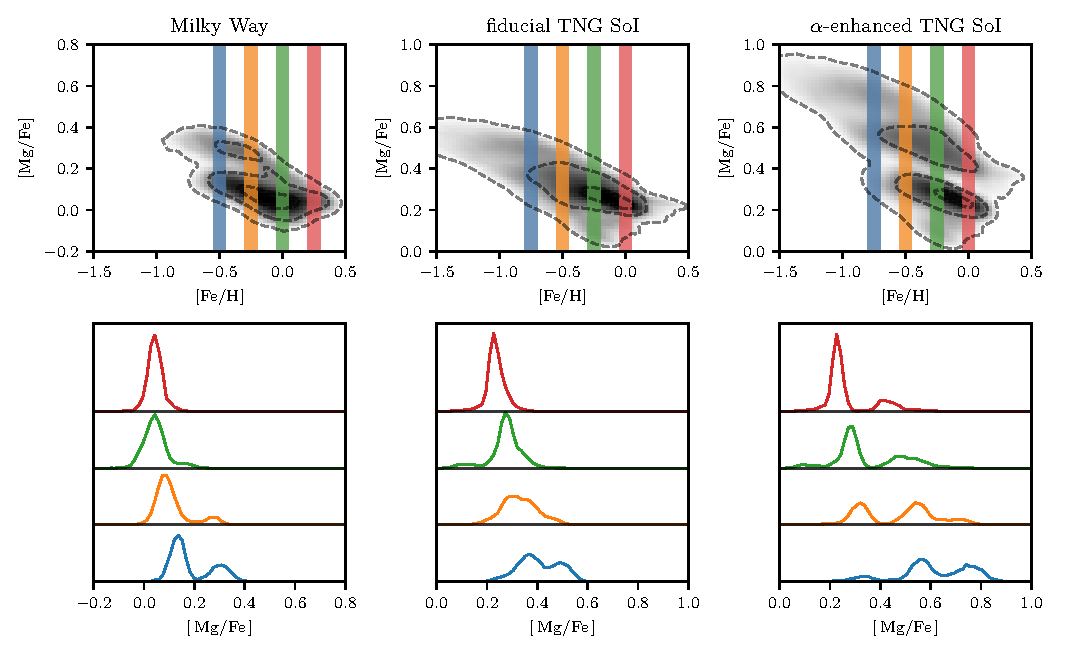
\includegraphics[width=\textwidth]{ch4/392276.pdf}
  \caption{\textbf{When old stars are $\alpha$-enhanced, our galaxy from TNG displays a prominent bimodality.} The upper left panel shows the distribution in the \MgFe{}-\FeH{} plane of the Milky Way, demonstrating a clear bimodality (data selection given in text). The lower left panel shows the 1D histograms of \MgFe{} at fixed \FeH{} values of $-0.5$, $-0.25$, $0$, and $0.25$ (blue, orange, green, and red, respectively). In the Milky Way, the bimodality is strongest at low metallicities while disappearing at high metallicities. The middle column shows the same plots but for our TNG galaxy (392276) and with the fixed \FeH{} values $0.25\,\dex$ lower. Only faint structure is seen in the lowest bin (blue, $-0.75\,\dex$). The right column shows the same subhalo but after increasing the \MgFe{} value of star particles formed before $z=1.5$ linearly with formation time (with a slope of $0.1\dex/\Gyr$). A clear bimodality is shown in these panels which, unlike in the Milky Way, is present at all metallicities.}
  \label{fig:fig1}
\end{figure*}

The main result of our paper is given in Figure~\ref{fig:fig1}. Here, we compare the abundance plane in the Milky Way (left column) to that of our TNG galaxy (middle and right columns). The upper panels show the 2D distribution in the space of \MgFe{}-\FeH{}. We have applied the standard \texttt{scipy} implementation of a Gaussian kernel density estimator to a Cartesian grid of points. For each panel, we normalize so that the integral of the distribution is unity. Colors are plotted in a log scale ranging from $0.08$ to $15\,\dex^{-2}$. Dashed contour lines are plotted at $0.1$, $1.5$, and $10\,\dex^{-2}$.

The colored vertical regions are indicated at $\FeH=-0.75$, $-0.5$, $-0.25$, and $0\,\dex$ in the Milky Way, and at bins $0.25\,\dex$ higher in the simulations. The lower panels show 1D histograms of \MgFe{} in bins centered on these values. The bins have width $0.1\,\dex$, which is reflected in the width of the colored, shaded regions in the upper panels. The rationale for the higher plotted \FeH{} in the simulations reflects the empirical location of the bimodalities. The Milky Way shows a clear bimodal population, with a high-$\alpha$ sequence most clearly distinct from the low-$\alpha$ sequence at low metallicity. The two sequences merge around solar metallicity.

Our galaxy, on the other hand, does not show a clearly bimodal structure in the fiducial simulation (middle column). There is some structure in the $\FeH=-0.75$ bin. The right panel of Figure~\ref{fig:fig1} shows the same distribution as in the middle panel, but with a modification to increase \MgFe{} values of older stars formed before $z=1.5$ (see Sections~\ref{ssec:tng} and \ref{ssec:onezone}, as well as the upper panels of Figure~\ref{fig:alpha} for a visual demonstration). A multimodal structure emerges with three clear modes at $\MgFe\sim0.8$, $0.5$, and $0.2\,\dex$. The 1D histograms show that the modes are well-separated, and that the troughs between the modes nearly vanish.

\subsection{Alpha Time Dependence}\label{ssec:alpha_time}

\begin{figure*}
  \centering
  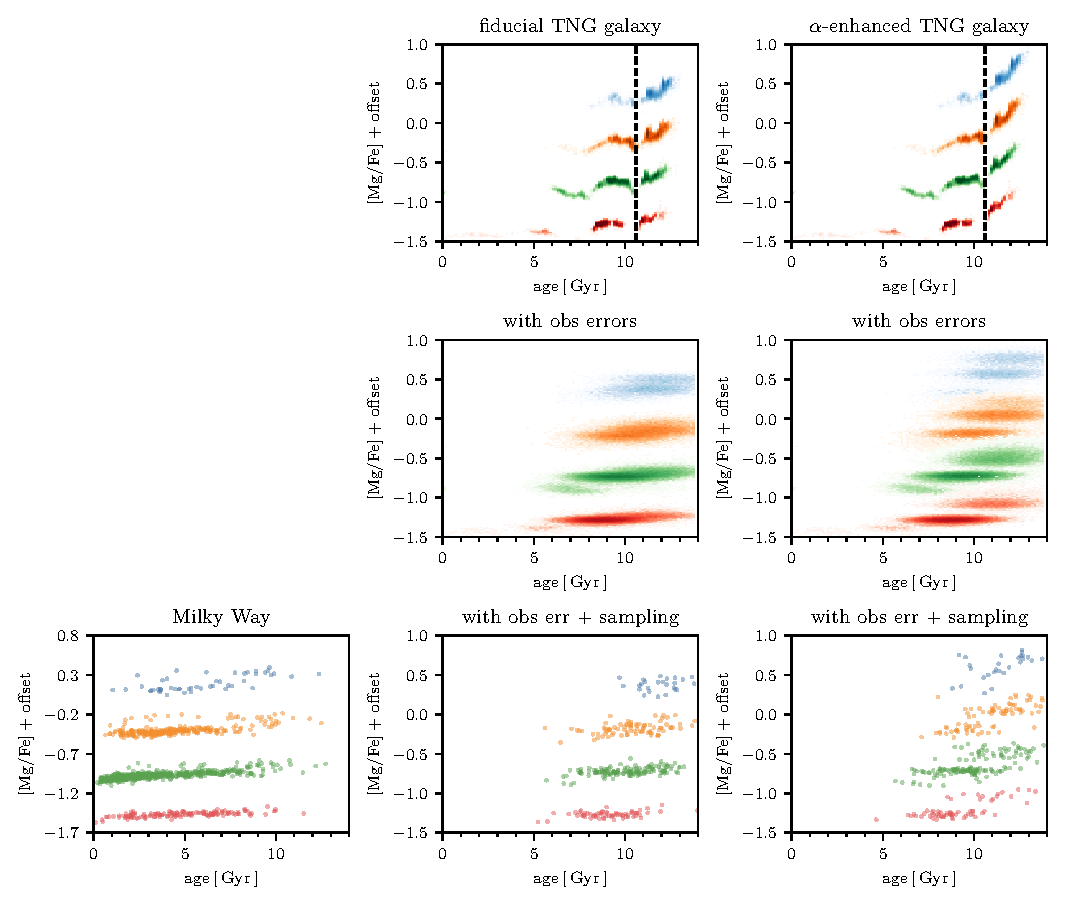
\includegraphics[width=\textwidth]{ch4/392276_alpha.pdf}
  \caption{\textbf{Bimodality in the abundance plane is linked to distinct epochs separated by quiescence in simulation.} The upper row shows \MgFe{} as a function of age for our subhalo in TNG. The colors indicate stellar populations at fixed values of \FeH{}, which are the same as in Figure~\ref{fig:fig1}. A gap in the relation occurs at an age of approximately $10.6\,\Gyr$, which we indicate with a vertical dashed line. The effect of the $\alpha$-enhancement is clear, as it separates the stars that form before and after this gap in ages (star particles which formed before $z=1.5$ are $\alpha$-enhanced, which occurs at an age of $\sim9.5\,\Gyr$). The middle row shows the same TNG and $\alpha$-enhanced TNG data, but with added uncertainties of $12.5\%$ in age and $0.015\,\dex$ in \MgFe{}. When given these errors, the before and after star particles smear such that the two populations significantly overlap in ages. There is a second population of stars linked to another gap at $\sim8\,\Gyr$, discussed in the text. The lower row shows on the left the Milky Way data and on the right the same TNG data with artificial errors but subsampled to the same number of stars older than $5\,\Gyr$ as in the observations (because the simulation sample has almost no star particles younger than $5\,\Gyr$). The limited sample size of the observations makes a direct comparison difficult.}
  \label{fig:alpha}
\end{figure*}

The abundance distributions shown in Figure~\ref{fig:fig1} can be better understood by examining the evolution of \MgFe{} with time of the individual stars/star particles. In the upper panels of Figure~\ref{fig:alpha} we show the true distribution of \MgFe{} as a function of time for the fiducial galaxy in the middle and for the post-processed, $\alpha$-enhanced subhalo to the right. We use age instead of formation time in order to better facilitate comparisons to observations. These panels show 2D histograms, with a logarithmic colormap normalized to the maximum of the plot. To prevent overlap, the values of \MgFe{} are given offsets of $0$, $-0.5$, $-1$, and $-1.5\,\dex$, in order of increasing \FeH{}.

In our simulated galaxy, there is an age gap at $\sim10.6\,\Gyr$, which we mark with a vertical dashed line in the upper row. Star particles older than this line have a much clearer gradient in time with \MgFe{} than stars that form after, even in the fiducial case. In the $\FeH=-0.25$ bin, star particles which form directly after this line have a slightly reduced \MgFe{} than stars which form a short time later.

In the middle row, the center and right panels show the simulated galaxies with Gaussian errors of $12.5\%$ in age and $0.015\,\dex$ in \MgFe{}, aligning with the observational uncertainties in the APOKASC-3 and APOGEE datasets (see Appendix~\ref{ch4:app:obs_err}). The error in \MgFe{} is insignificant, but the age error ($1.25\,\Gyr$ at $10\,\Gyr$) significantly blurs the distribution, particularly across the dashed line that marks the transition between sequences. Despite this, the $\alpha$-enhanced galaxy still shows two distinct populations, although their ages now overlap more significantly.

The upper and middle row shows that there is a potential third population of star particles in the simulation, which is most visible in the $\FeH=-0.25$ and $0\,\dex$ bins (green and red, respectively). A minor gap in the upper panels is present at an age of $\sim8\,\Gyr$, which we discuss further in Section~\ref{ssec:evol}.

The lower row compares Milky Way data (left) with simulations of fiducial (middle) and $\alpha$-enhanced (right) galaxies. Here, the simulations have been subsampled to match the observed sample size of stars older than $5\,\Gyr$ in each metallicity bin. We match the sample size only to old stars because our simulated sample has almost no star particles younger than $5\,\Gyr$. When subsampled with observational errors, the $\FeH=-0.5$ bin in the simulation (orange right panel) very faintly shows a hint of two stacked distributions which might also be present in the $\FeH=-0.25$ bin in the data (orange left panel). The limited sample size makes it impossible to draw any strong conclusions.

\subsection{Evolutionary History}\label{ssec:evol}
\begin{figure}
  \centering
  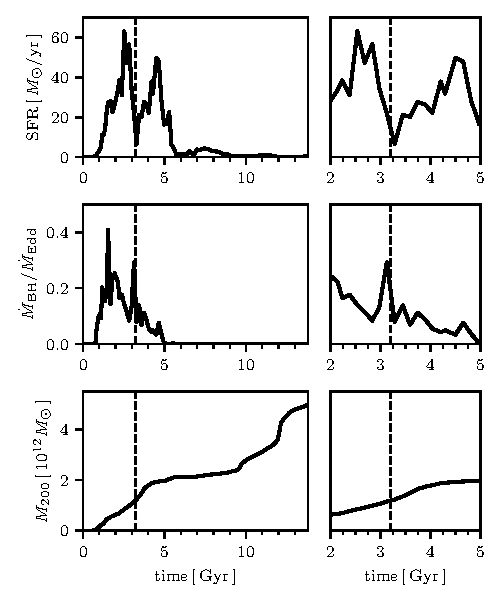
\includegraphics[width=208.14452628pt]{ch4/392276_SFH_AGN_M200.pdf}
  \caption{\textbf{The evolutionary history of our TNG galaxy.} The left column shows the SFH, BH accretion rate, and virial mass ($M_{200}$) over the entire time span, while the right column zooms in on the period from $t=2\,\Gyr$ to $t=5\,\Gyr$. The vertical dashed line in each panel marks the transition at $t\sim3.2\,\Gyr$, corresponding to the separation between the high- and low-$\alpha$ sequences (as shown in Figure~\ref{fig:alpha}). The upper panel shows the SFH, the middle panel shows the BH accretion rate as a fraction of the Eddington limit, and the lower panel shows the virial mass, representing the mass enclosed within a radius where the density is $200\times$ the mean cosmic density.}
  \label{fig:history}
\end{figure}

To understand the key events driving the behavior around the dashed line in Figure~\ref{fig:alpha}, we examine the evolution of several properties of our galaxy in Figure~\ref{fig:history}: its SFH, the BH accretion rate, and the growth of the virial mass. The vertical dashed line in each panel marks the transition at $t\sim3.2\,\Gyr$ from the high- to low-$\alpha$ sequences, as in Figure~\ref{fig:alpha}. The upper panel in the left column shows the the SFR (computed for all gas cells in the \texttt{SUBFIND} subhalo). There are two peaks at $t\sim2.5\,\Gyr$ and $t\sim4.5\,\Gyr$ with maximum values of $50\,\Msun/\textrm{yr}$ and $30\,\Msun/\textrm{yr}$, respectively. Around the high- to low-$\alpha$ transition, there is a dip in the SFR, which drops by an order of magnitude to about $3\,\Msun/\textrm{yr}$. The right panel zooms in on the period between $t=2\,\Gyr$ and $5\,\Gyr$, where we observe a sharp recovery in the SFR following the quiescent phase. In the span of a single snapshot (roughly $150\,\Myr$), the SFR increases from about $3\,\Msun/\textrm{yr}$ to $10\,\Msun/\textrm{yr}$.

There is also a more minor period of quiescence at a cosmic time of $\sim6\,\Gyr$, followed by a period of SF at a much lower rate. This is likely linked to the third population separated by an age gap at $\sim8\,\Gyr$ seen in Figure~\ref{fig:alpha}.

The middle panels track the accretion rate of the central BH as a fraction of the Eddington rate. Early in our galaxy's history ($t<2\,\Gyr$), the BH experiences high accretion, which steadily declines until $t\sim5\,\Gyr$. Around $t\sim3.2\,\Gyr$, the BH accretion rate peaks again, reaching approximately $30\%$ of the Eddington limit, placing the BH in quasar mode and injecting significant thermal energy into the galaxy's center. The middle right panel shows the period between $t=2$ and $5\,\Gyr$. We can see that the decline in the galaxy's SFR is contemporaneous with this increase in the BH accretion rate.

The lower panel illustrates the growth of the galaxy's virial mass ($M_{200}$). Early on ($t<4\,\Gyr$), $M_{200}$ increases roughly linearly, reaching about $2 \times 10^{12}\,\Msun$. After this, the mass remains relatively stable until jumps occur around $t\sim10$ and $\sim12\,\Gyr$, indicative of mergers. These late-time mergers raise the virial mass to $5 \times 10^{12},\Msun$, well above the typical Milky Way estimate of $1$--$1.5\times 10^{12},\Msun$ \citep[e.g.][]{2016ARA&A..54..529B}. However, during the high- to low-$\alpha$ transition, the virial mass remains consistent with a Milky Way progenitor, making this galaxy a suitable analog. There are no mergers related to the earlier quiescent period around $t\sim3.2\,\Gyr$ (no major mass jumps are observed during this time), implying the AGN activity is not merger-driven. The lower right panel shows the lack of mergers in more detail during the period between $t=2$ and $5\,\Gyr$.

As discussed in Paper~I, the key to generating an $\alpha$-bimodality is halting star formation within specific metallicity ranges. A global quiescent period is a sufficient but not necessary condition for the formation of such gaps. To illustrate this point, we present Figure~\ref{fig:zSFH}, which compares the global SFH in black with the SFH in narrow metallicity bins, color-coded to match the bins shown in Figure~\ref{fig:fig1}. This plot uses the $z=0$ distribution of star particle formation times, resulting in minor differences from the SFH shown in Figure~\ref{fig:history}. Notably, we observe a significant drop in the SFR within these metallicity bins, lasting up to $\sim1\,\Gyr$. However, because the timing of these metallicity-dependent gaps differs, the total SFR never falls below $\sim10\,\Msunyr$.

\begin{figure}
  \centering
  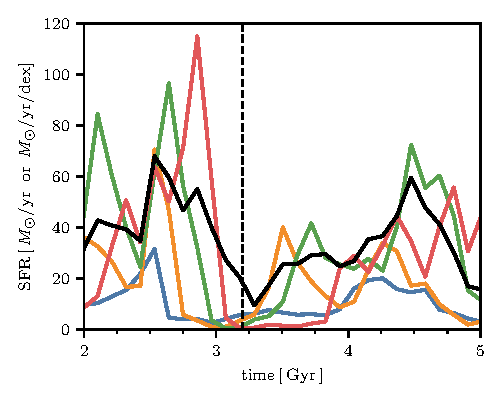
\includegraphics[width=208.14452628pt]{ch4/392276_zSFH.pdf}
  \caption{Global star formation history (black) compared with the star formation history in narrow metallicity bins, color-coded as in Figure~\ref{fig:fig1}. This plot demonstrates that the key condition for generating an $\alpha$-bimodality, the cessation of star formation in specific metallicity ranges, is satisfied. The metallicity-dependent SFR drops nearly to zero in every bin for periods extending up to $\sim1\,\Gyr$. The timing and duration of metallicity-dependent gaps can vary, preventing the total SFR from falling below $\sim10\,\Msunyr$.}
  \label{fig:zSFH}
\end{figure}

\subsection{Bar-Driven Quenching}\label{ssec:sequence_of_events}
\begin{figure*}
  \centering
  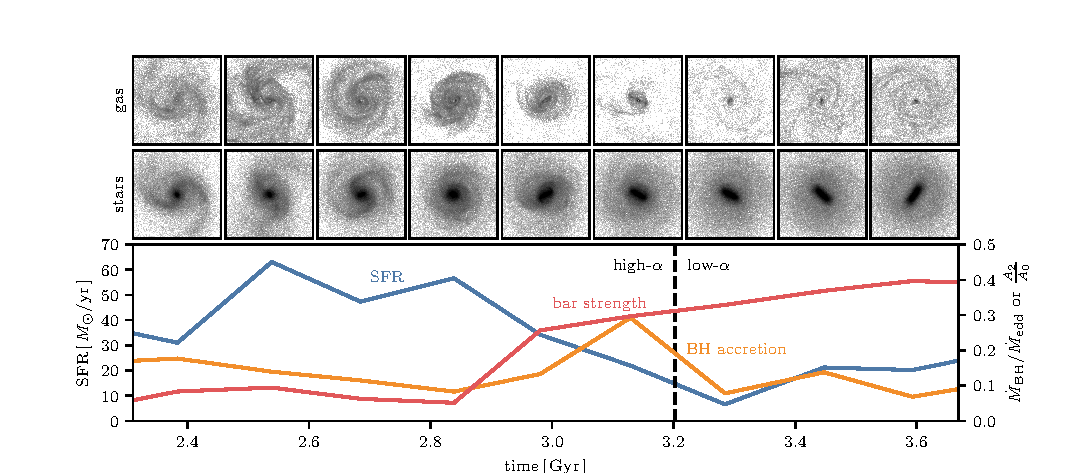
\includegraphics[width=\textwidth]{ch4/alyssa.pdf}
  \caption{\textbf{Quiescence separating the high- and low-$\alpha$ sequences is preceded by AGN activity associated with bar formation.} Surface density projections of gas (top row) and star particles (middle row) in our galaxy across snapshots at different times during the high- to low-$\alpha$ transition. Below the projections is a plot showing the SFR, BH accretion rate (in units of $\dot{M}_{\textrm{BH}}/\dot{M}_{\textrm{edd}}$), and bar strength ($A_2/A_0$ for $R<2$ kpc). Time ranges from $\sim2.4\,\textrm{Gyr}$ to $\sim3.6\,\textrm{Gyr}$, corresponding to redshifts from $z\sim2.7$ to $z\sim1.8$. A sequence of events in which the bar strengthens, BH accretion increases, and SFR declines is seen, and is described more fully in the text.}
  \label{fig:seq}
\end{figure*}

We find that a quenching episode is driven by the formation of a bar contemporaneous with an increase in AGN activity, shown in Figure~\ref{fig:seq}. The upper panels show gas density, while the middle panels display stellar density. Time progresses from $\sim2.4$ to $\sim3.6\,\textrm{Gyr}$, corresponding to redshifts ranging from $z\sim2.7$ to $z\sim1.8$, and the high- to low-$\alpha$ transition is indicated with a vertical dashed line.

This figure shows the following sequence of events:
\begin{enumerate}
    \item Bar forms: A steady increase in the bar strength, as indicated by $A_2/A_0$ for star particles with $R<2\,\kpc$, from $\sim0.05$ to $0.4$ starting around $2.8\,\textrm{Gyr}$. This rise is accompanied by the appearance of elongated features in the gas and stars consistent with a bar.
    \item BH accretion increases: Following the increase in bar strength by about a snapshot ($\sim150\,\Myr$ here), the BH accretion rate ($\dot{M}_{\textrm{BH}}/\dot{M}_{\textrm{edd}}$) shows a significant spike, rising from a minimum of $\sim0.08$ at $t=2.84\,\Gyr$ to a maximum of $\sim0.29$ at $t=3.13\,\Gyr$ for one snapshot.
    \item SFR declines: The SFR declines starting from a maximum of $54.3\,\Msunyr$ at $t=2.84\,\Gyr$ down to $3.6\,\Msunyr$ at $t=3.28\,\Gyr$. In the next snapshot at $t=3.45\,\Gyr$ the SFR recovers to $12.2\,\Msunyr$. Figure~\ref{fig:history} shows that it reaches its second maximum of $30.9\,\Msunyr$ at $4.5\,\Gyr$. We show in Figure~\ref{fig:zSFH} that the global SF suppression is coincident with a much more dramatic metallicity dependent SF gap, with the SFR dropping nearly to $0\,\Msunyrdex$ in several bins.
\end{enumerate}

Note that in the Milky Way the bar is estimated to have formed approximately $8\,\Gyr$ ago \citep{2019MNRAS.490.4740B,2024MNRAS.530.2972S}, coinciding with the epoch when the bimodality is observed to emerge \citep{2013A&A...560A.109H,2023MNRAS.525.2208R,2024MNRAS.535..392L}.

\subsection{\alphaFe{} with Varying SFE}\label{ssec:onezone}

\begin{figure}
  \centering
  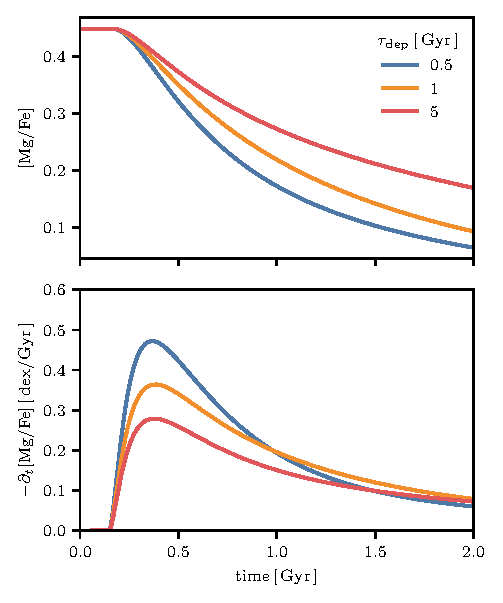
\includegraphics[width=208.14452628pt]{ch4/mgfe_vice.pdf}
  \caption{\textbf{A higher star formation efficiency leads to a steeper decline in \MgFe{}.} In both panels, the lines show the time evolution of \MgFe{} in a simple one-zone chemical evolution model, described in Section~\ref{ssec:onezone_met}. The evolution for different SFE values of $2$, $1$, and $0.2\,\textrm{Gyr}^{-1}$ are shown in blue, orange, and red, respectively.  The upper panel shows the evolution of \MgFe{} over $2\,\Gyr$, while the lower panel shows the negative of its time derivative. Increasing the SFE (decreasing $\tau_{\textrm{dep}}$) leads to a more rapid decline in \MgFe{}. At its steepest decline ($t\sim0.5\,\Gyr$), increasing the SFE by an order of magnitude results in a slope nearly twice as steep. At later times ($t > 1\,\Gyr$), models with higher SFE reach their steady-state \MgFe{} value more quickly.}
  \label{fig:vice}
\end{figure}

In Figure~\ref{fig:fig1}, we showed that a time-linear $\alpha$-enhancement of older stars (formed before $z=1.5$) leads to the emergence of a pronounced chemical bimodality. This $\alpha$-enhancement corresponds to a more rapid decline in \alphaFe{} over time at high redshifts. Here we show that the steeper \alphaFe{} evolution implied by this $\alpha$-enhancement of old stars can be physically justified as a boost to the SFE of dense gas.

The evolution of \MgFe{} in three one-zone GCE models with varying SFEs is shown in the upper panel of Figure~\ref{fig:vice} (models described in Section~\ref{ssec:onezone_met}). A higher SFE (lower $\tau_{\textrm{dep}}$) leads to a faster reduction in \MgFe{}. In the model with the highest SFE ($2\,\Gyr^{-1}$, $\tau_{\textrm{dep}}=0.5\,\Gyr$, blue), \MgFe{} drops from $\sim0.45$ to $0.08\,\dex$ over $2\,\Gyr$. In contrast, the model with the lowest SFE ($0.2\,\Gyr^{-1}$, $\tau_{\textrm{dep}}=5\,\Gyr$, red) only reaches $\sim0.2\,\dex$ within the same period.

The lower panel shows the negative time derivative of \MgFe{} (i.e., the rate of decline). The model with the highest SFE ($2\,\Gyr^{-1}$, blue) has a peak decline rate of $-0.5\,\dex/\Gyr$, while the model with the lowest SFE ($0.2\,\Gyr^{-1}$) peaks at $-0.25\,\dex/\Gyr$. After $1\,\Gyr$, the trend begins to reverse, and the lower-SFE models catch up, though at a much slower rate ($\sim-0.1\,\dex/\Gyr$) compared to their peak.

This analysis illustrates that a higher SFE at early times (high-$z$) leads to a faster decline in \MgFe{}. Recent work has suggested that the SFE in such dense regions in TNG may indeed be too low, as discussed in Section~\ref{ssec:sfe}. The post-processing $\alpha$-enhancement in Section~\ref{ssec:tng} is meant to mimic a SFE correction of high-$z$ dense gas.

\section{Discussion}\label{sec:disc}
In Figure~\ref{fig:fig1}, we compared the abundance plane between the Milky Way and our galaxy before and after our $\alpha$-enhancement post-processing procedure. It is clear that the TNG galaxy is unimodal before the $\alpha$-enhancement and multi-modal afterwards. Here, we briefly discuss two main points: (1) assuming the $\alpha$-enhancement is justified, what leads to the bimodality in the TNG galaxy?, and (2) what justifies the $\alpha$-enhancement? We then extend our comparison to data and argue the quiescent period is driven by a bar-induced AGN episode.

\subsection{Cause of Bimodality}\label{ssec:bim_cause}
We argue that the available evidence for the cause of the bimodality aligns with the scenario outlined in Paper~I. That study presented an idealized simulation resembling the merger between the Milky Way and GSE, where the orbital parameters were varied slightly across a grid of 27 simulations. The results showed that simulations featuring a brief quiescent period produced a bimodal abundance distribution. Two conditions for the bimodality to arise have to be met: (1) a declining \alphaFe{} with time (here done through our post-processing step, see Figure~\ref{fig:alpha}), and (2) a gap in the metallicity-dependent SFR. In Paper~I, the gap in SFR was due to a merger, but here we argue it is due to the formation of a bar.

The galaxy that we have studied in this work is consistent with the quiescent scenario proposed in Paper~I. The distribution of \MgFe{} with star particle age is a useful way to test this scenario, which we plot in the upper right panel of Figure~\ref{fig:alpha} in fixed bins of \FeH{} (each color is a different \FeH{} bin). The vertical dashed line at $z\sim2$ in Figures~\ref{fig:alpha} and \ref{fig:history} marks the transition between the high- and low-$\alpha$ sequences.
\footnote{The transition between the high- and low-$\alpha$ sequences occurs approximately $1\,\Gyr$ before $z=1.5$, where the $\alpha$-enhancement begins. This, combined with the fact that not all of the subhalos in our sample display bimodalities (Appendix~\ref{ch4:app:rand_fig1}), shows that the $\alpha$-enhancement is not the direct cause of the bimodality.} At the transition, there is a $\sim300\,\Myr$ quiescent period during which the SFR drops by a factor of $\sim10$ to $15$.

This global quiescent period is symptomatic of a more dramatic reduction in the star formation rate in narrow metallicity bins, which almost entirely vanishes (Figure~\ref{fig:zSFH}). As we showed in Paper~I, it is the metallicity-dependent quiescence in the presence of a declining gas-phase \MgFe{} -- not global quiescence -- that leads to an $\alpha$-bimodality. In the fiducial TNG model, the \MgFe{} reduction with time is not rapid enough, leading to the post-processing discussed in Section~\ref{ssec:sfe}. In the real universe, a global quiescent period of a duration of $\sim300\,\Myr$ would lead to a reduction in enrichment from Type~II relative to Type~Ia SNe leads to a lower rate of Mg production. The typical lifetime of a Type~II SN progenitor in this model is $\sim40\,\Myr$ \citep{2018MNRAS.473.4077P}, and so the hundreds of Myr of suppressed SF would be short enough to restrict the production of $\alpha$-elements.

In the fiducial TNG distribution, shown in the upper middle panel of Figure~\ref{fig:alpha}, the same general behavior is present. However, because the \MgFe{} decline before the quiescent period is slower, star particles which formed before and after this period overlap in the \MgFe{} distribution shown in Figure~\ref{fig:fig1}.

Notably, both the fiducial and $\alpha$-enhanced galaxy show a slight rebound effect in \MgFe{}. The star particles which form directly after the dashed line when the SFR has just recovered have a slightly lower \MgFe{} than stars which form later on, by about $0.1$ to $0.2\,\dex$. We argue that it is plausible that during the period of suppressed star formation, the \alphaFe{} ratio of the star-forming gas drops sharply due to the reduced contribution of Type~II relative to Type~Ia SNe. Later, the \alphaFe{} of the gas will recover when the SFR also recovers, but there is a brief window when old, low-$\alpha$ stars can form. A similar behavior was seen in the one-zone models with bursty SFHs in \citet{2020MNRAS.498.1364J}.

\subsection{Motivation for $\alpha$ Post-processing}\label{ssec:sfe}
As described in Section~\ref{ssec:tng}, we applied a post-processing which increased the \MgFe{} of star particles at $z>1.5$ in a time-linear manner, discussed in Section~\ref{ssec:tng}. The post-processed subhalo is presented alongside the fiducial subhalo in the right and middle columns, respectively, of Figures~\ref{fig:fig1} and \ref{fig:alpha}.

The \MgFe{} value of star forming gas is the result of a complicated mixture of many different aspects of the TNG model, to name a few: stellar and AGN feedback which alter gas inflows and outflows, secular, dynamical evolution, SF prescription, magnetic fields, (lack of) cosmic rays, diffusivity of hydrodynamics solver, and, of course, enrichment models. Isolating the cause of the potentially too shallow evolution of \MgFe{} vs. time at high-$z$ is not straightforward nor, in our opinion, even possible. However, we do offer one reasonable explanation: the SFE at high densities, more present at high-$z$, is too low.

We demonstrate the impact of the SFE on the \alphaFe{} ratio using a simple one-zone chemical evolution model with the publicly available code \texttt{VICE}. The details of our setup is given in Section~\ref{ssec:onezone_met}. We vary the SFE of the model ($\textrm{SFR}/M_{\textrm{gas}}$), and examine the impact on \MgFe{} as a function of time. We find that a higher SFE does lead to a more rapid reduction in \MgFe{}. The rate of decrease in \MgFe{}, at its maximum, varies between $\sim-0.25$, $-0.35$, and $-0.5\,\dex/\Gyr$ in the $\textrm{SFE}=0.2$, $1$, and $2\,\Gyr^{-1}$ models, respectively. For our post-processing, we assumed an additional decrease rate of $0.1\,\dex/\Gyr$. Such a difference is well within the range of \MgFe{} slopes seen in our different $\tau_{\textrm{dep}}$ models, implying a factor of only $\sim2$ to $5$ in the SFE is needed to reach our post-processing slope.

The TNG model predicts depletion times at high gas surface densities ($\tau_{\textrm{dep}}\sim0.5-1\,\Gyr$ at $\Sigma_{\textrm{gas}} ~ 100-300\,\Msun/\pc^2$) which are a factor of $\sim2$--$3$ longer than derived for starburst galaxies at similar densities of $\tau_{\textrm{dep}}\sim30$--$300\,Myr$ assuming \citet{2013ARA&A..51..207B} X(CO) \citep[see][]{2019ApJ...872...16D,2021ApJ...908...61K,2024arXiv240909121H}. This is well within our needed factor of $\sim2$ to $5$ in the SFE (see Figure~\ref{fig:vice}). Therefore, \MgFe{} should decline more rapidly with a different feedback model (or future iteration of the TNG model) that leads to a higher SFE at high densities.

An intuitive understanding of the impact the decline in \alphaFe{} vs. time has is that, when \alphaFe{} declines rapidly, it is a better estimator of age. When \alphaFe{} is a better estimator of age, events which are separated temporally become better separated in the abundance plane.

\subsection{Direct Comparison to Observations}\label{ssec:compare_obs}
We attempted a direct comparison between our TNG galaxy and the Milky Way in the lower row of Figure~\ref{fig:alpha} (see Section~\ref{ssec:alpha_time}). In the simulations, the presence of the bimodality is obvious from a stacked distribution. However, this distribution is not obvious in the observations, primarily because the sample size of observations at old ages where the bimodality is present ($>5\,\Gyr$) is quite small. Nonetheless, the presence of a clean gap in stellar ages between the high- and low-$\alpha$ is completely washed out by the age uncertainties.

There is also a population of young, $\alpha$-rich stars in the APOKASC-3 data. These may or may not reflect the typical or average ISM chemistry. Arguments have been made that they are old stars with misclassified astroseismic ages due to binary mass transfer \citep[and references therein]{2023A&A...671A..21J}. However, some appear to be genuinely young \citep[and references therein]{2024arXiv241002962L}, with a range of explanations given \citep[e.g.][]{2015A&A...576L..12C,2021MNRAS.508.4484J,2023arXiv231105815S}. Disentangling these effects is far from clear and beyond the scope of this work. At least some of the young, $\alpha$-rich stars in Figure~\ref{fig:alpha} do not reflect the ISM chemistry at their inferred astroseismic age, and so would not be included in the TNG model. With this caveat, the two appear to be consistent.

\subsection{Cause of Quiescence}\label{ssec:cause_qui}
In Paper~I, AGN activity from a merger was the suspected cause for the quiescent period. In our galaxy here, there is indeed a brief burst in AGN accretion at the time of the merger (middle panel of Figure~\ref{fig:history}). Based on this burst, it is also reasonable to suspect that AGN activity is also responsible for the quiescent period in our galaxy, noting that the real cause of the formation of the $\alpha$-bimodality is a metallicity-dependent quiescent period (see Paper~I and Figure~\ref{fig:zSFH}). However, we argued in Section~\ref{ssec:sequence_of_events} that the cause of the localized spike in the BH accretion rate is not due to a merger but instead due to the formation/strengthening of a bar. This connection is further supported by estimates that the Milky Way's bar formed $\sim8\,\Gyr$ ago \citep[e.g.,][]{2019MNRAS.490.4740B,2024MNRAS.530.2972S}, roughly concurrent with the formation of the bimodality \citep{2013A&A...560A.109H,2023MNRAS.525.2208R,2024MNRAS.535..392L}.

There is a significant body of theoretical and observational work in support of this picture. Bars and other non-axisymmetric features have long been argued to funnel gas into the centers of galaxies on theoretical grounds \citep{1989Natur.338...45S,2010MNRAS.407.1529H}. It was recently shown by \citet{2024arXiv240906783F} that bars can induce quiescence by accelerating the growth of a SMBH, but they found there can be many Gyr between bar formation and quenching. In observations, barred galaxies preferentially host AGN in star-forming galaxies \citep{2012ApJS..198....4O,2022A&A...661A.105S}.\footnote{\citet{2022A&A...668L...3L} studied a galaxy from TNG100 in which a merger induced AGN activity that ejected gas from its center. A bar then formed out of the gas-poor disk.} Furthermore, at high-$z$, the AGN mechanism is thought to be responsible for quenching \citep[e.g.][and references therein]{2023arXiv230806317D,2024arXiv240417945P,2024ApJ...968L..21M,2024Natur.630...54B}.

Since barred galaxies preferentially host AGN, we therefore predict that barred galaxies would preferentially host $\alpha$-bimodalities. The GECKOS survey, which aims to constrain the $\alpha$-bimodality of a sample of edge-on galaxies, about half of which are barred, using integral field spectroscopy at different altitudes, could test this \citep[and J. v.~d.~Sande, private communication]{2024IAUS..377...27V}. On the other hand, the strength of a bar is not associated with the strength of the host AGN \citep[e.g.]{2022A&A...661A.105S}. So, it is not clear that bimodalities would be associated with bar strength.

A complicating factor for this picture comes from the high SFR associated with the galaxy. The depletion time ($M_{\textrm{gas}}/\textrm{SFR}$) at the $t=2.84\,\Gyr$ snapshot is $204\,\Myr$, shorter than the time it takes for the SFR to reach its minimum. This implies the possibility of starvation as a quenching mechanism. However, the average depletion time in the preceding 5 snapshots (which are each $\sim150\,\Myr$ apart) is $220\,\Myr$, so clearly the galaxy is accreting high amounts of gas from its environment. A definitive account, difficult with the current simulation outputs because of its sparse snapshot spacing, requires further work. We also delay to future work the cause of the secondary quiescence period at $\sim6\,\Gyr$, briefly discussed in Section~\ref{ssec:evol}.

\section{Conclusions}\label{sec:conc}
In this work, we examined a galaxy in Illustris TNG50 which is at a Milky Way-progenitor mass at $z=1.5$. After applying a post-processing step that increased the \MgFe{} of star particles formed before $z=1.5$, this subhalo hosts a strong bimodality in the plane of \MgFe{} and \FeH{}, shown in Figure~\ref{fig:fig1}. This post-processing is justified by arguing that the SFE of dense gas is too low in TNG \citep[][see discussion in our Section~\ref{ssec:sfe}]{2024arXiv240909121H}.

The formation of the bimodality, when the galaxy transitions from producing high- to low-\MgFe{} star particles (Figure~\ref{fig:alpha}), is coincident with both a global and metallicity-dependent suppression of star formation (Figures~\ref{fig:history} and \ref{fig:zSFH}). This suppression of star formation is preceded by the formation of a bar and subsequent AGN activity (Figure~\ref{fig:seq}). This scenario is plausible for the Milky Way, as recent estimates indicate that the bar formed around $8\,\Gyr$ ago \citep{2019MNRAS.490.4740B,2024MNRAS.530.2972S}, coinciding with the onset of the bimodality.

The lack of star formation in a narrow metallicity bin in the presence of a decline in \MgFe{} naturally leads to a gap in the present-day distribution of \MgFe{} (see Paper~I). However, in the fiducial TNG  model, the decline in \MgFe{} is not rapid enough during the period of quiescence to produce an $\alpha$-bimodality. Our post-processing $\alpha$-enhancement artificially injects this declination. In the real universe, a global reduction in the SFR may expedite the drop in \MgFe{} since the number of Type~II relative to Type~Ia SNe would drop.

This work adds further support to a scenario in which a quiescent period in the Milky Way's past is a plausible explanation for the Milky Way's abundance bimodality. We argued in Paper~I that the GSE merger could trigger this period. In this work we have argued that the formation of the Milky Way's bar could be responsible. Regardless of this scenario's relevance to the Milky Way, we also predict that the presence of a bar in external galaxies is correlated with the presence of an $\alpha$-bimodality. Because of observational errors in age, it is not possible to make a direct comparison between the simulated galaxy and dataset (Figure~\ref{fig:alpha} and Section~\ref{ssec:compare_obs}). In the future, more numerous and precise age estimates of old, metal-poor stars may be able to distinguish the formation scenarios of the $\alpha$-bimodality.

\section{Acknowledgements}
We would like to thank the referee for a thoughtful and helpful report. We would like to thank Marc Pinsonneault and Jesse van de Sande for helpful discussions, and M. Pinsonneault for sharing early access to the APOKASC-3 dataset. AB would like to thank Todd Phillips for helpful discussions.

  JWJ acknowledges support from a Carnegie Theoretical Astrophysics Center postdoctoral fellowship. Support for VS was provided by Harvard University through the Institute for Theory and Computation Fellowship. LH acknowledges support by the Simons Collaboration on ``Learning the Universe.''

  This work has made use of data from the European Space Agency (ESA) mission {\it Gaia} (\url{https://www.cosmos.esa.int/gaia}), processed by the {\it Gaia} Data Processing and Analysis Consortium (DPAC, \url{https://www.cosmos.esa.int/web/gaia/dpac/consortium}). Funding for the DPAC has been provided by national institutions, in particular the institutions participating in the {\it Gaia} Multilateral Agreement.
  
  Funding for the Sloan Digital Sky 
  Survey IV has been provided by the 
  Alfred P. Sloan Foundation, the U.S. 
  Department of Energy Office of 
  Science, and the Participating 
  Institutions. 
  
  SDSS-IV acknowledges support and 
  resources from the Center for High 
  Performance Computing  at the 
  University of Utah. The SDSS 
  website is www.sdss4.org.
  
  SDSS-IV is managed by the 
  Astrophysical Research Consortium 
  for the Participating Institutions 
  of the SDSS Collaboration including 
  the Brazilian Participation Group, 
  the Carnegie Institution for Science, 
  Carnegie Mellon University, Center for 
  Astrophysics | Harvard \& 
  Smithsonian, the Chilean Participation 
  Group, the French Participation Group, 
  Instituto de Astrof\'isica de 
  Canarias, The Johns Hopkins 
  University, Kavli Institute for the 
  Physics and Mathematics of the 
  Universe (IPMU) / University of 
  Tokyo, the Korean Participation Group, 
  Lawrence Berkeley National Laboratory, 
  Leibniz Institut f\"ur Astrophysik 
  Potsdam (AIP),  Max-Planck-Institut 
  f\"ur Astronomie (MPIA Heidelberg), 
  Max-Planck-Institut f\"ur 
  Astrophysik (MPA Garching), 
  Max-Planck-Institut f\"ur 
  Extraterrestrische Physik (MPE), 
  National Astronomical Observatories of 
  China, New Mexico State University, 
  New York University, University of 
  Notre Dame, Observat\'ario 
  Nacional / MCTI, The Ohio State 
  University, Pennsylvania State 
  University, Shanghai 
  Astronomical Observatory, United 
  Kingdom Participation Group, 
  Universidad Nacional Aut\'onoma 
  de M\'exico, University of Arizona, 
  University of Colorado Boulder, 
  University of Oxford, University of 
  Portsmouth, University of Utah, 
  University of Virginia, University 
  of Washington, University of 
  Wisconsin, Vanderbilt University, 
  and Yale University.

We acknowledge the use of OpenAI’s ChatGPT and Anthropic's Claude for assistance in editing this manuscript for clarity and conciseness and in generating small analysis scripts and code snippets.

We have made use of the following software: {\sc astropy} \citep{astropy:2013,astropy:2018,astropy:2022}, {\sc h5py} \url{http://www.h5py.org/}, {\sc inspector\_gadget} \url{https://bitbucket.org/abauer/inspector_gadget/}, {\sc joblib} \url{https://joblib.readthedocs.io/en/latest/}, {\sc matplotlib} \citep{Hunter:2007}, {\sc numba} \citep{lam2015numba}, {\sc numpy} \citep{harris2020array}, {\sc scikit-learn} \citep{scikit-learn}, {\sc scipy} \citep{2020SciPy-NMeth}, {\sc tqdm} \url{https://tqdm.github.io/}, {\sc vortrace} \url{https://github.com/gusbeane/vortrace}


\chapter{Conclusions}\label{ch:conclusions}
% !TEX root = ../ms.tex

\begin{adjustwidth}{.8cm}{0cm}
\textit{I therefore, if you are a person of the same sort as myself, should be glad to continue questioning you: if not, I can let it drop. Of what sort am I? One of those who would be glad to be refuted if I say anything untrue, and glad to refute anyone else who might speak untruly; but just as glad, mind you, to be refuted as to refute, since I regard the former as the greater benefit, in proportion as it is a greater benefit for oneself to be delivered from the greatest evil than to deliver some one else. For I consider that [one] cannot suffer any evil so great as a false opinion on the subjects of our actual argument.}

\hspace{9cm} -- Socrates
\end{adjustwidth}

\hfill \break
\noindent
This thesis has explored two key observational facts about the Milky Way. First, its bar is both old and fast-rotating. Second, at low metallicities there is a bimodal distribution in the stellar surface abundance of $\alpha$-elements. We examined the physical mechanisms behind these features via idealized numerical simulations.

In Chapter~\ref{ch:gasbar}, we proposed a solution to why the Milky Way's bar is both old and rotating rapidly. Although the bar should, in principle, lose angular momentum to the dark matter halo through resonant orbital interactions (thus slowing its pattern speed), the gas phase of the galaxy exerts a positive torque that arrests the dynamical friction process responsible for the halo's negative torque. In our simulations, this interplay effectively ``locks'' the bar at nearly constant speed over many Gyr. Our result explains why most observed bars are fast rotators without appealing to exotic physics, and suggests that slowly rotating bars should occur in gas-poor galaxies such as lenticulars.

We then turned to the emergence of the $\alpha$-bimodality in Chapter~\ref{ch:GSEgas}. In the \alphaFe--\FeH{} plane, the Milky Way separates into high- and low-$\alpha$ sequences. While there are many proposed explanations for this structure, including the sudden infusion of gas by the Gaia-Sausage-Enceladus merger, we presented a new mechanism where a short-lived ($\sim300\,\Myr$) cessation of star formation at a particular metallicity naturally produces a bimodal \alphaFe{} distribution. This scenario predicts a narrow age gap for $\sim8\,\Gyr$ old stars at $\FeH \lesssim -0.2$.

Building on these ideas, we showed in Chapter~\ref{ch:Mgdec} that bar formation in a galaxy from the cosmological simulation Illustris~TNG50 can itself drive a global quenching event, splitting the high- and low-$\alpha$ populations through a similar gap in star formation. Hence, we predict that barred galaxies should show a higher prevalence of $\alpha$-bimodalities than unbarred ones.

In current research on the Milky Way, theory struggles to keep pace with the abundance and precision of observed stellar dynamics and abundances. This gap will only widen as even more precise measurements become available. SDSS-V will soon deliver millions of abundances \citep{2017AJ....154...94M}, while the proposed Maunakea Spectroscopic Explorer will measure tens to hundreds of millions abundances down to a g-band magnitude of $20$ over its lifetime \citep{2023AN....34430108S}. But what do we actually gain from measuring so many abundances? To wit, this thesis has proposed a new explanation for the abundance bimodality that was discovered in 2011 with a sample of 1112 stars \citep{2011A&A...535L..11A} using simulation techniques developed shortly after that discovery. Will measuring abundances for a factor of 10,000 more stars truly clarify the origin story of the Milky Way? In our view, we have just started on the antipasti with the primi already on the table -- untouched -- and the secondi in the waiter's hands trying to find a place to set it down.

We need high-precision stellar ages -- in particular, of the old, metal-poor stars that the Galaxy's history is written in. A productive direction to explore in this regard comes from two complementary approaches which show particular promise: differential spectral analysis and gyrochronology measurements in combination. Differential spectral analysis has achieved remarkable precision for solar twins, reaching age uncertainties of $\sim400\,\Myr$ \citep{2018MNRAS.474.2580S}, but extending this technique to metal-poor stars has never been explored. Combining spectroscopic parameters with rotation periods from stellar light curves has been shown to improve age precision by up to a factor of 3, though the effectiveness varies across different stellar populations \citep{2019AJ....158..173A}. We plan to explore all these considerations. Nonetheless, high-precision stellar ages would truly unlock the Milky Way's history, but at the moment no one has the key.

Many years remain in this golden age of Milky Way science.

%%%%%%%%%%%%%%%% BACK MATTER %%%%%%%%%%%%%%%%

% Put appendices, bibliography, and supplemental materials here

% The bibliography may be single spaced within each entry, but must be
% double-spaced between each entry. Most bibliography styles leave space between
% entries, so that shouldn't be a problem.
\begin{singlespacing}
  % I like "References" better than "Bibliography"
  \renewcommand{\bibname}{References}

  % Any bibliohgraphy style that leaves space between entries is fine
  \bibliographystyle{aasjournal}
  \bibliography{ref}
\end{singlespacing}

% Appendices from all chapters should go at the end
% !TEX root = ms.tex

\begin{appendices}

\chapter{Appendix to Chapter~\ref{ch:gasbar}}\label{ch:app_gasbar}
\section{Bar Decomposition}
\label{ch2:app:bardecomp}
\begin{figure*}
    \centering
    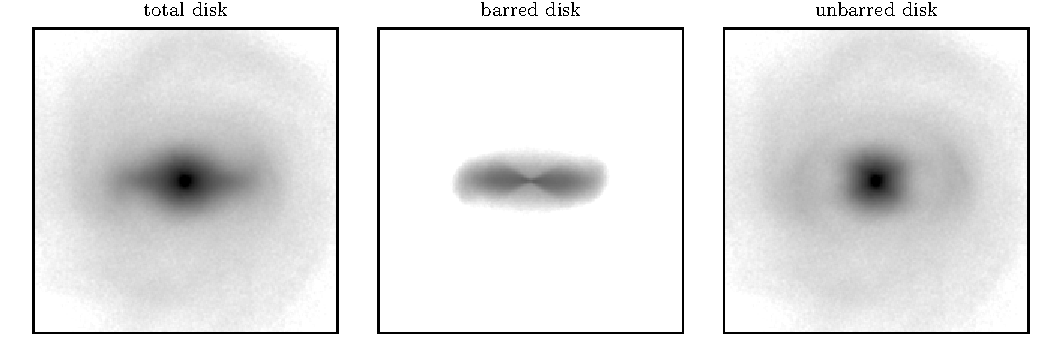
\includegraphics[width=\textwidth]{ch2/fig/bar_decomp.pdf}
    \caption{Disk decomposition into the barred and unbarred disk. This
    procedure is based on \citet{2016MNRAS.463.1952P}. The \textit{left panel}
    shows a face-on surface density projection through the stellar component of
    the \SMUGGLE{} simulation (disk and bulge) at $t=1\,\textrm{Gyr}$. The
    \textit{middle panel} shows the component of the disk identified as being
    trapped in the bar while the \textit{right panel} shows the component of the
    disk identified as not being trapped in the bar. The fact that the untrapped
    stars form a roughly axisymmetric structure indicates our bar decomposition
    is sufficiently accurate. We have computed that $76\%$ of the second Fourier
    component resides in the stars classified as being trapped in the bar.}
    \label{fig:decomp}
\end{figure*}

Computing the length of the bar and the torque on the bar by different
components requires us to decompose the disk into a component which is trapped
by the bar and a component which is untrapped. In order to do this, we follow
closely the technique developed in \citet{2016MNRAS.463.1952P}. We analyzed the
orbit of each star particle (meaning initial disk, bulge, and newly formed
stars) by extracting the $x$-$y$ positions of the apoapse of each in a frame
corotating with the bar, where apoapses are defined as local maxima in $r$. For
each apoapse, we searched for the $19$ closest apoapses in time and applied a
$k$-means clustering algorithm on this set of $20$ points with $k=2$. We then
computed for each of the two clusters the average angle from the bar
$\left<\Delta \phi\right>_{0,1}$, the standard deviation in $R$ of the points
${\sigma_R}_{0,1}$, and the average radius of the cluster
$\left<R\right>_{0,1}$. At each apoapse, a particle was considered to be in the
bar if it met the following criteria:
\begin{equation}
\textrm{max}\left(\left<\Delta \phi\right>_{0,1}\right) < \pi / 8
\end{equation}
\begin{equation}
\frac{{\sigma_R}_0 + {\sigma_R}_1}{\left<R\right>_0 + \left<R\right>_1} < 0.22
\end{equation}
These criterion are slightly different and simplified from the ones used in
\citet{2016MNRAS.463.1952P}, but we found them to empirically work well at
decomposing the disk into a bar and disk component. In Fig.~\ref{fig:decomp}, we
show an example of this decomposition. The \textit{left} panel shows a surface
density projection of the stellar disk and bulge (including newly formed stars)
from the \SMUGGLE{} model after $1\,\text{Gyr}$ of evolution in a frame such that
the bar is aligned with the $x$-axis. The \textit{middle} panel shows a
projection of the subset of stars that are identified as being trapped in the
bar and the \textit{right} panel shows a projection of the stars that are not
identified as being trapped. The fact that the \textit{right} panel is roughly
axisymmetric indicates the bar decomposition is performing adequately.

We computed the second Fourier component $A_2$ for all particles classified as
barred and unbarred. We found that $76\%$ of the total $m=2$ Fourier component
is in the particles classified as barred (i.e.,
$A_{2,\textrm{bar}}/A_{2,\textrm{tot}}\sim0.76$). Some of this is probably
coming from the $m=4$ component (e.g., boxy orbits) being classified as
unbarred, or the presence of weak spiral arms. See also
\citet{2021MNRAS.500..838P} for more details on the orbit family breakdown.

\section{Varying Pattern Speed}
\label{ch2:app:varyps}
When the bar slows down, we argue that this induces a larger positive torque
from the gas phase. Only gas within corotation will flow inwards, while gas
outside corotation will flow outwards \citep{2011MNRAS.415.1027H}. Since the
corotation radius is larger for more slowly rotating bars, it follows that
more slowly rotating bars should be more efficient at driving gas inflows and
thus experience a larger positive torque from the gas phase.

We performed an experiment to test this hypothesis by freezing the stellar
disk in the \SMUGGLE{} run and forcing it to rotate at a constant angular rate.
This has the effect of forcing the bar to rotate as a solid body at a constant
angular rate which we control. The gas is evolved self-consistently with this
rotating disk. We measured the torque on the bar by the gas phase at different
rotation rates. The result of this experiment is illustrated in
Fig.~\ref{fig:equil}, which shows that a more slowly rotating bar experiences a
larger positive torque from the gas.

We also note that since \citet{2011MNRAS.415.1027H} predicts gas outside of
corotation will flow outward, the bar should exert a positive torque on that
gas. Indeed, we measured the average torque on gas outside corotation from
$t=3\,\textrm{Gyr}$ to $5\,\textrm{Gyr}$ to be $0.87$ in code units
($10^{10}\,M_{\odot}\,(\text{km}/\text{s})^2$). For reference, the average
torque inside corotation is $-10.8$ over the same time period and in the same
units. So, while gas outside corotation does experience a positive torque, the
total torque on the gas phase is still negative.

\begin{figure*}
    \centering
    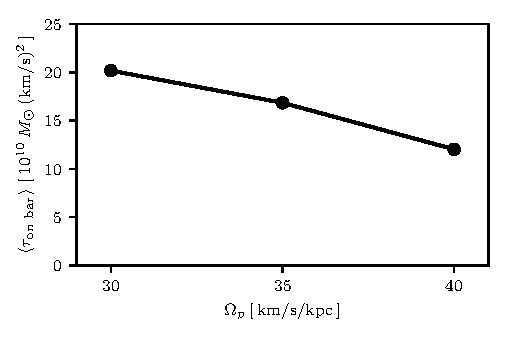
\includegraphics[width=9cm]{ch2/fig/torque_ps.pdf}
    \caption{Average torque exerted by gas on a bar which rotates at a fixed
    pattern speed. Since only gas within the corotation radius is able to infall
    and slower bars have larger corotation radii, slower bars experience a
    larger net torque than faster bars. The setup of the simulations used here
    is identical to the \SMUGGLE{} case discussed earlier, except the \Nbody{} disk
    is rotated as a solid body with a constant angular
    velocity.}
    \label{fig:equil}
\end{figure*}

\begin{figure*}
    \centering
    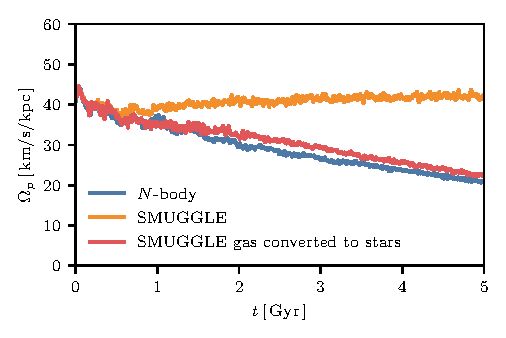
\includegraphics[width=9cm]{ch2/fig/ps_star.pdf}
    \caption{Pattern speed evolution of a model in which we instaneously
    add stars instead of gas to the simulation, with the same density profile as
    the gas phase. The pattern speed evolution in this case is qualitatively
    similar to that of the $N$-body case, with a slight offset in the pattern
    speed. This test demonstrates that the stable pattern speed evolution in the
    SMUGGLE case is not simply a consequence of the change in potential imposed
    in our initial conditions.}
\label{fig:ps-star}
\end{figure*}

\section{Stars Instead of Gas}
In the SMUGGLE model considered in this work, we instantaneously added gas to
the $N$-body system after $1.5\,\textrm{Gyr}$ of evolution. One might wonder if
this sudden change to the potential is responsible for the stable pattern speed
evolution. To test whether this is the case, we added mass to the system in the
same way we did for the SMUGGLE model, but using collisionless particles instead
of gas. The result of this experiment is shown in Fig.~\ref{fig:ps-star}. While
there is an offset compared to the pure $N$-body case, we see that the pattern
speed evolution is broadly consistent with a declining pattern speed. This
indicates that the gas phase is responsible for the stable pattern speed.

\begin{figure}
    \centering
    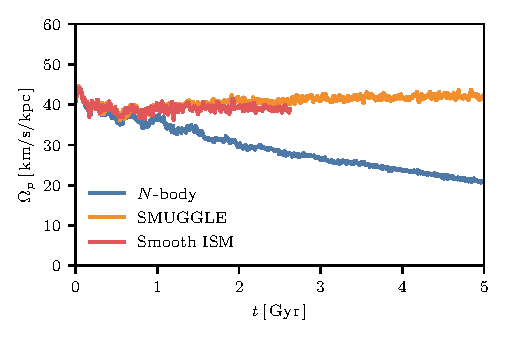
\includegraphics[width=9cm]{ch2/fig/ps_GFM.pdf}
    \caption{Pattern speed evolution of a smooth ISM model. This evolution is
    shown for the fiducial disk in the \Nbody{} (blue), \SMUGGLE{} (orange), and
    smooth ISM (red) cases. The smooth ISM model is an older model for the ISM
    which treats its multiphase nature in a subgrid fashion
    \citep{2003MNRAS.339..289S}. This fundamentally differs from the \SMUGGLE{}
    model, which explicitly resolves the hot and cold phases of the ISM
    \citep{2019MNRAS.489.4233M}. The pattern speed in the smooth ISM case is
    broadly similar to the evolution in the \SMUGGLE{} case. This shows that the
    stability of the pattern speed is not simply a result of our assumed model
    for the ISM.}
\label{fig:GFM}
\end{figure}

\section{Smooth Interstellar Medium}
We performed a simulation of the same disk but with a simpler model of the
interstellar medium \citep{2003MNRAS.339..289S}, closer to standard methods used
in cosmological simulations of galaxy formation and described in more detail in
Section~\ref{ch2:sec:methods}. The result of this test is presented in
Fig.~\ref{fig:GFM}. We find that the pattern speed evolution is nearly the same
in this case, and so conclude that our result is not sensitive to the details of
the model for the interstellar medium.

\section{Semi-Analytic Model Parameters}
\label{ch2:app:sam}
Our semi-analytic model consisted of a three-component bar-disk-halo system. We
describe here the parameters we chose for these components. The parameters of
the disk and halo were chosen to match closely what we used in our fiducial
simulations. The system can thus be understood as being roughly similar to the
Milky Way, though no careful analysis has been performed to ensure the closest
match possible.

For the dark matter halo, we used a Hernquist potential
\citep{1990ApJ...356..359H} with mass $10^{12}\,\Msun$ and a scale length of
$26.2\,\textrm{kpc}$. For the stellar disk, we used a Miyamoto-Nagai disk
\citep{1975PASJ...27..533M} with mass $4.8\times10^{10}\,\Msun$, radial scale
length of $2.67\,\textrm{kpc}$, and vertical scale length of
$0.32\,\textrm{kpc}$. For the bar, we used the quadrupole potential described in
\citet{2022MNRAS.513..768C}. We used their fiducial parameter values --
specifically, we set $A=0.02$, $b=0.28$, and $v_c = 235\,\kms$. Our initial
pattern speed is always set to $40\,\kms/\textrm{kpc}$.

We integrated our model for $5\,\textrm{Gyr}$ with a timestep of
$0.01\,\textrm{Gyr}$.

\section{Comparison to the Milky Way}
\label{ch2:app:milkyway}
For several Gyr, our fiducial disk exhibits several properties in reasonable
agreement to the Milky Way. This is uncommon in models of galaxies that include
the gas phase of the disk but no circumgalactic medium. As mentioned earlier,
the pattern speed seems to match the observed pattern speed of the Milky Way's
bar \citep{2019MNRAS.490.4740B}. We briefly summarize some of the other ways our
disk is comparable to the Milky Way.

We computed the circular velocity curve of our model using the \texttt{AGAMA}
package \citep{2019MNRAS.482.1525V}. We fit the baryonic component (stellar
disk, bulge, gas, and newly formed stars) with an axisymmetric cylindrical
spline with $20$ grid points in both the radial and vertical direction spanning
$0.2$ to $50\,\textrm{kpc}$ in the radial direction and from $0.02$ to
$10\,\textrm{kpc}$ in the vertical direction. We fit the dark matter halo using
an axisymmetric multipole fit with a maximum angular harmonic coefficient
of $l=2$, to account for the compression of the halo by the disk. We plot
the circular velocity curve at $t=1\,\textrm{Gyr}$ in Fig.~\ref{fig:vcirc}
compared to observational estimates \citep{2019ApJ...871..120E}. The \SMUGGLE{}
disk (which includes additional mass in the form of gas) has a slightly higher
circular velocity than the \Nbody{} disk which, itself, is slightly higher than
the observational estimates. Overall, though, the circular velocity curves
between our model and that observed in the Milky Way are broadly consistent.

We also show the evolution of the surface density profile in Fig.~\ref{fig:surf}
We find that in our simulation the atomic and molecular gas surface density and
the SFR surface density is broadly consistent with the expected values for the
Milky Way \citep{2008A&A...487..951K,2022ApJ...929L..18E}. The discrepancy between
$1$ and $4\,\textrm{kpc}$ in the molecular and SFR surface density is probably due
to the fact that the distances to molecular clouds which underlines this work
used a simple kinematic distance based on an axisymmetric model of the Milky
Way \citep{2017ApJ...834...57M}, which is not accurate in the bar region where gas
has large non-circular velocities.

We measured the initial scale height of the atomic gas disk in a bin
extending from $R=7.5\,\textrm{kpc}$ to $R=8.5\,\textrm{kpc}$. The initial
vertical profile is well-fit by a Gaussian with a scale height of
$110\,\textrm{pc}$. At $t=1\,\textrm{Gyr}$, the vertical profile in the same
radial bin is better fit by an exponential profile with scale height of
$74\,\textrm{pc}$. These are somewhat lower than the observed value in the HI
disk of $\sim200\,\textrm{pc}$ \citep{1995ApJ...448..138M, 2017A&A...607A.106M}.
This may be caused by the model in our simulations not driving enough turbulent
pressure, and is an interesting avenue of further investigation.

\begin{figure*}
    \centering
    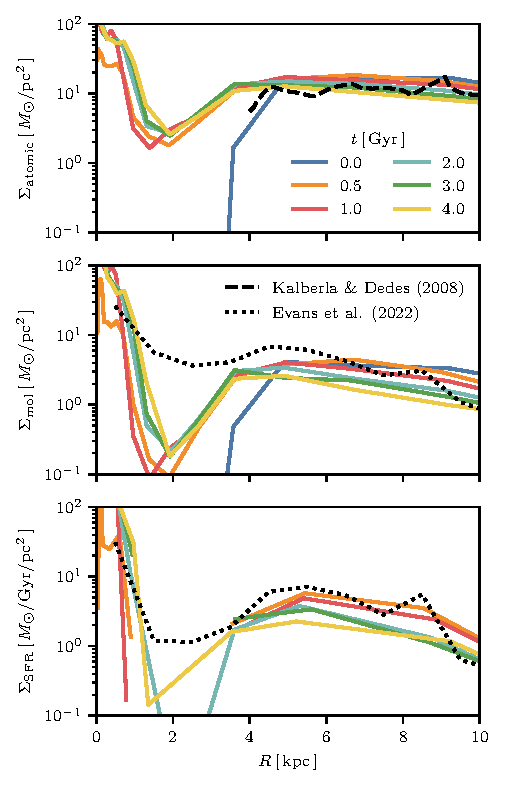
\includegraphics[width=9cm]{ch2/fig/surf_dens.pdf}
    \caption{The time evolution of the atomic gas surface density
    (\textit{upper}), molecular gas surface density (\textit{middle}) and the
    star formation rate (SFR) surface density (\textit{lower}) at various times
    during our fiducial simulation. Colored lines indicate the profiles at
    selected times during the simulation while the black dashed lines indicate
    observations for the atomic gas \citep{2008A&A...487..951K} and black dotted
    lines indicate a model which allows the CO-to-H$_2$ conversion factor
    $X_{\textrm{CO}}$ to vary with metallicity \citep{2022ApJ...929L..18E}.
    Molecular gas surface densities were provided separately (N. Evans, private
    communication). We see that the molecular gas and SFR surface densities are
    within an order of magnitude of the Milky Way's typical values at all times.
    We see a sharp decrease in the gas and SFR surface densities along the
    extent of the bar from $\sim1$ to $\sim4\,\textrm{kpc}$, related to the gas
    inflow in this region.}
    \label{fig:surf}
\end{figure*}

\begin{figure}
    \centering
    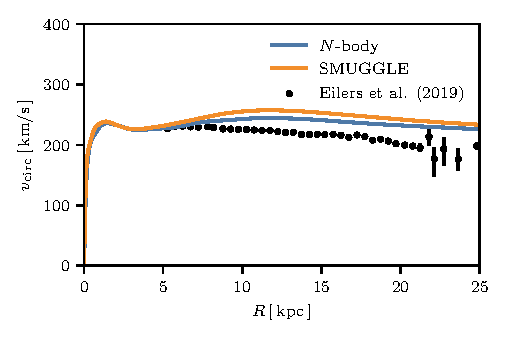
\includegraphics[width=9cm]{ch2/fig/vcirc.pdf}
    \caption{The circular velocity curve of our setups at $t=1\,\textrm{Gyr}$.
    This curve is shown for the \Nbody{} run (blue) and the \SMUGGLE{} run
    (orange) compared to observational estimates for the Milky Way
    \citep{2019ApJ...871..120E}. We see that the circular velocity curve for
    both runs is marginally larger than the Milky Way's, but still comparable.
    The \SMUGGLE{} circular velocity curve is larger than the \Nbody{} curve due
    to the additional mass in the gas phase.}
    \label{fig:vcirc}
\end{figure}

\chapter{Appendix to Chapter~\ref{ch:GSEgas}}\label{ch:app_GSEgas}

\section{Star Formation Histories}\label{ch3:app:all_sfh}
One potential avenue for creating an \FeH{}-dependent star formation gap is through quiescence. This is demonstrated by examining the global SFH in Figure~\ref{fig:all_sfh}, with the panels and colors showing each simulation in the grid ordered by their bimodality score $\mathcal{B}$ in the same way as Figures~\ref{ch3:fig:all_hist} and \ref{ch3:fig:all_scatter}. One can see that there is a global quiescent period in simulations~g, s, and x. Simulations~s and x have a bimodal pattern, while simulation~g has a unimodal pattern. As mentioned in Figure~\ref{ch3:fig:all_scatter}, simulation~g has an age gap but there is not enough star formation at $\FeH\sim0$ before the gap to result in a strong bimodality. Otherwise, while a global quiescent period is sufficient for generating an age gap, most simulations do not have a global quiescent period.

\begin{figure*}
  \centering
  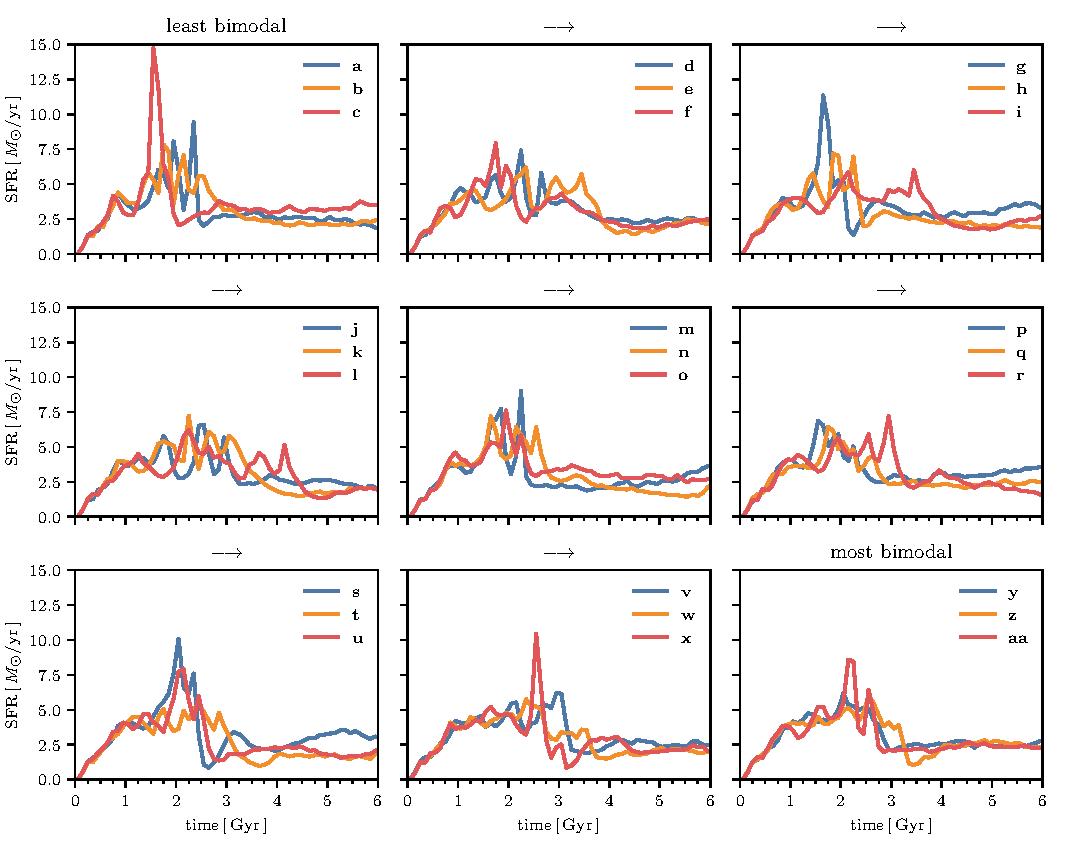
\includegraphics[width=\textwidth]{ch3/sfh.pdf}
  \caption{Global star formation history (SFH) for each simulation, plotted in the same order as Figures~\ref{ch3:fig:all_hist} and \ref{ch3:fig:all_scatter}, with increasing bimodality score $\mathcal{B}$ from left to right. The colors correspond to the same simulations as in previous figures. A global quiescent period, characterized by a significant dip in the SFR, is observed in simulations~g, s, and x. Among these, simulations~s and x exhibit strong bimodal \MgFe{} distributions, while simulation~g remains unimodal due to insufficient early star formation at $\FeH\sim0$ before the quiescent phase. Most other simulations do not display a clear global quiescent period, indicating that such a phase is not strictly necessary for bimodality to emerge.}
  \label{fig:all_sfh}
\end{figure*}

\section{Cause of Suppressed Star Formation}\label{ch3:app:cause_qui}
In Figure~\ref{fig:MdotBH_rsep}, we demonstrate how the orbit of the bimodal simulation is closely related to the strength of BH feedback. On the $y$-axis, we show in blue the black hole accretion rate as a ratio of the maximum (Eddington) accretion rate at that time. In orange we show the orbital separation between the satellite and central galaxies. We see that the accretion rate is high early on at $\sim10\%$. At the time around coalescence at $\sim2\,\Gyr$, the accretion rate rises up to Eddington, before dropping to a much lower value $<10\%$ later on.

In the TNG model, the strength of AGN feedback is directly tied to the BH's accretion rate \citep{2017MNRAS.465.3291W}. Therefore, it is reasonable to suspect that the feedback from the AGN is responsible for removing gas from the galaxy or keeping it above the star forming density threshold.

\begin{figure}
  \centering
  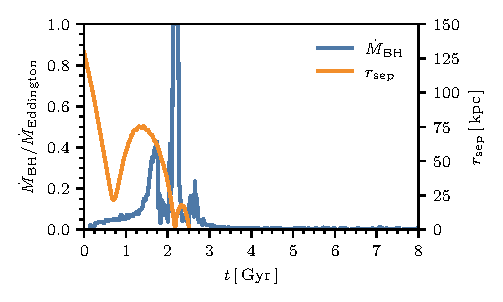
\includegraphics[width=242.26653pt]{ch3/MdotBH_rsep.pdf}
  \caption{Evolution of black hole accretion rate and orbital separation over time in the bimodal simulation. The blue line shows the black hole accretion rate as a fraction of the Eddington rate, while the orange line shows the orbital separation between the satellite and central galaxies. The accretion rate peaks during coalescence at $\sim2\,\Gyr$, suggesting a strong connection between the merger and AGN activity.}
  \label{fig:MdotBH_rsep}
\end{figure}

\section{Abundance Plane of All Simulations}\label{ch3:app:allmerge}
We show summary plots of the abundance planes of all simulations in our orbital grid in Figures~\ref{fig:allmerge0} to \ref{fig:allmerge8}.

\begin{figure*}
  \centering
  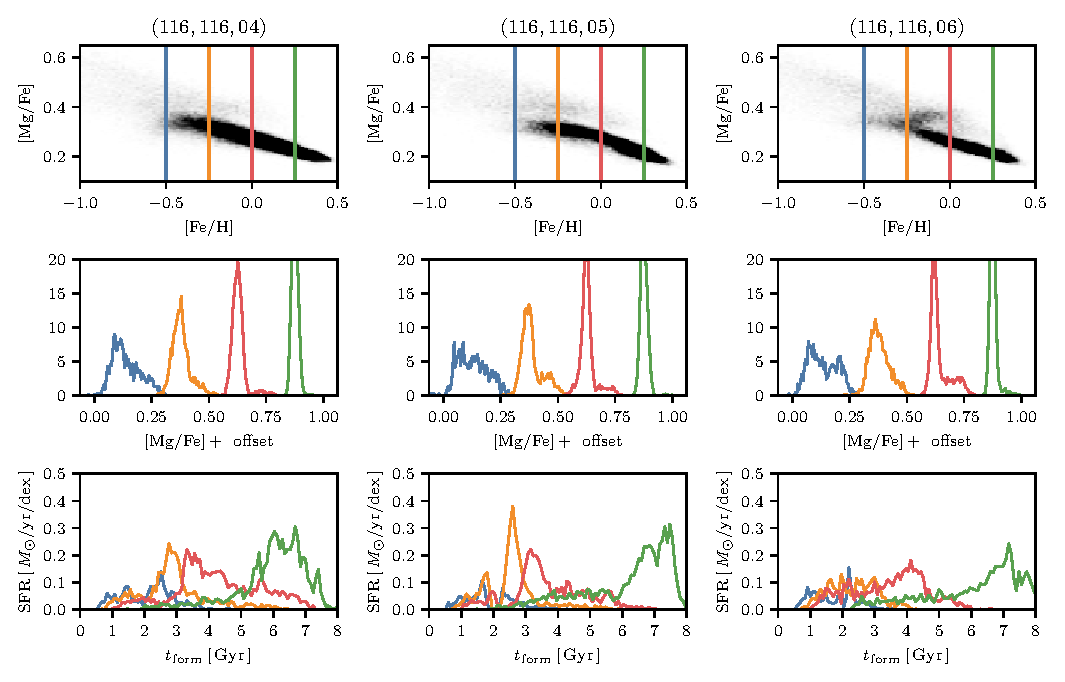
\includegraphics[width=\textwidth]{ch3/allmerge0.pdf}
  \caption{A summary of the abundance plane and star formation history of all simulations within the orbital grid. Each figure shows the outcome of a simulation at a fixed $R_0$ and $V_0$, varying $\eta$. The title of each column shows the $R_0$, $V_0$, and $\eta$ of that simulation, in order. The upper and middle rows replicate Figure~\ref{ch3:fig:fig1}, which show the distribution of stars in the abundance plane of \MgFe{}-\FeH{} as well as 1D histograms at a fixed \FeH{} of $-0.5$, $-0.25$, $0$, and $0.25$. The lower rows replicate Figure~\ref{ch3:fig:before_after_sfh_by_iron}, showing the star formation history at each \FeH{}.}
  \label{fig:allmerge0}
\end{figure*}

\begin{figure*}
  \centering
  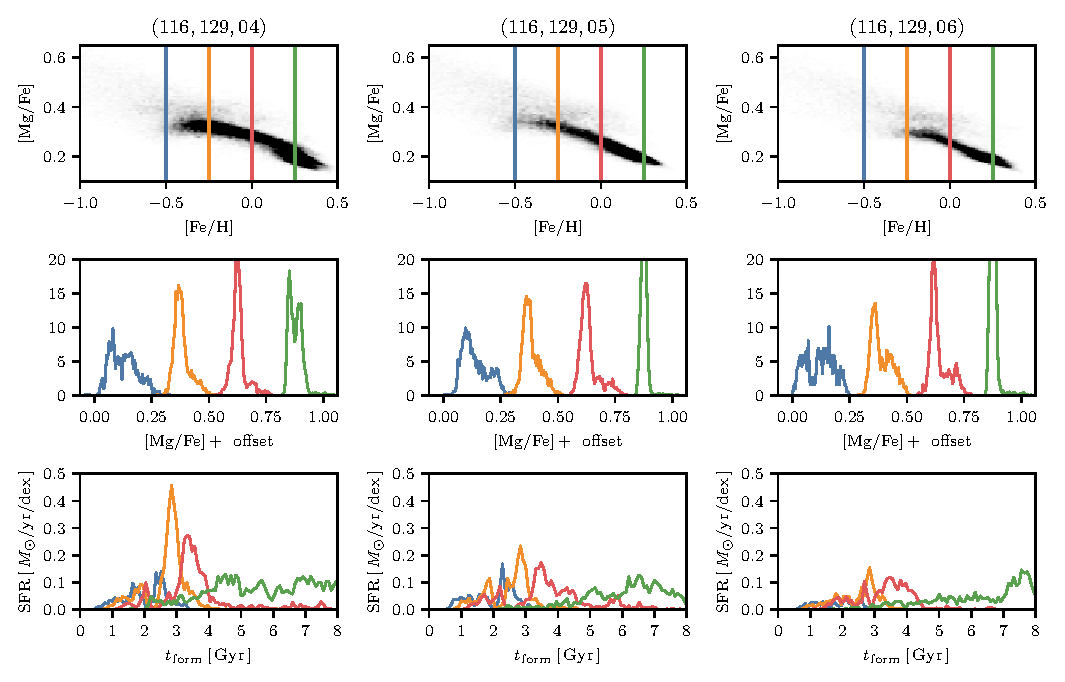
\includegraphics[width=\textwidth]{ch3/allmerge1.pdf}
  \caption{A continuation of Figure~\ref{fig:allmerge0}.}
  \label{fig:allmerge1}
\end{figure*}

\begin{figure*}
  \centering
  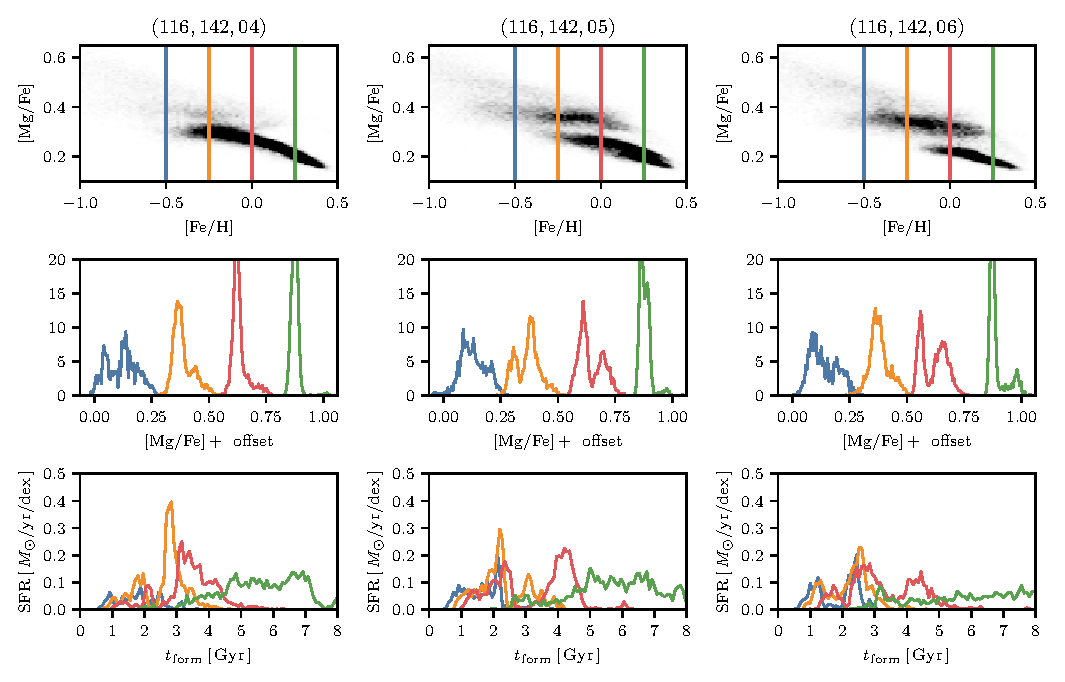
\includegraphics[width=\textwidth]{ch3/allmerge2.pdf}
  \caption{A continuation of Figure~\ref{fig:allmerge0}.}
  \label{fig:allmerge2}
\end{figure*}

\begin{figure*}
  \centering
  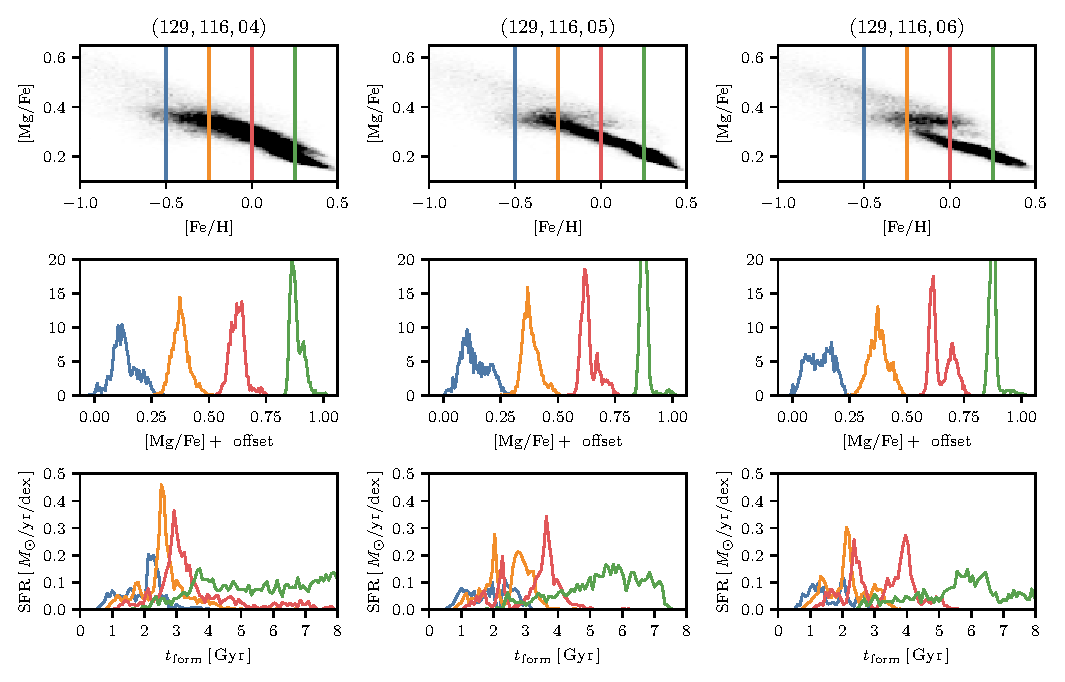
\includegraphics[width=\textwidth]{ch3/allmerge3.pdf}
  \caption{A continuation of Figure~\ref{fig:allmerge0}.}
  \label{fig:allmerge3}
\end{figure*}

\begin{figure*}
  \centering
  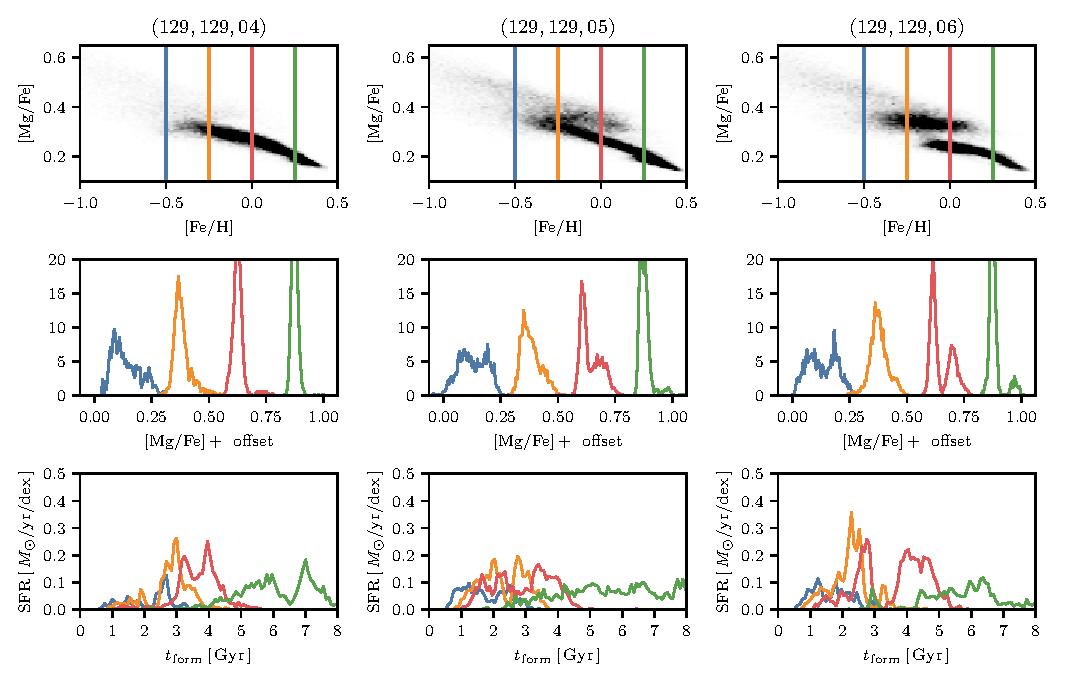
\includegraphics[width=\textwidth]{ch3/allmerge4.pdf}
  \caption{A continuation of Figure~\ref{fig:allmerge0}.}
  \label{fig:allmerge4}
\end{figure*}

\begin{figure*}
  \centering
  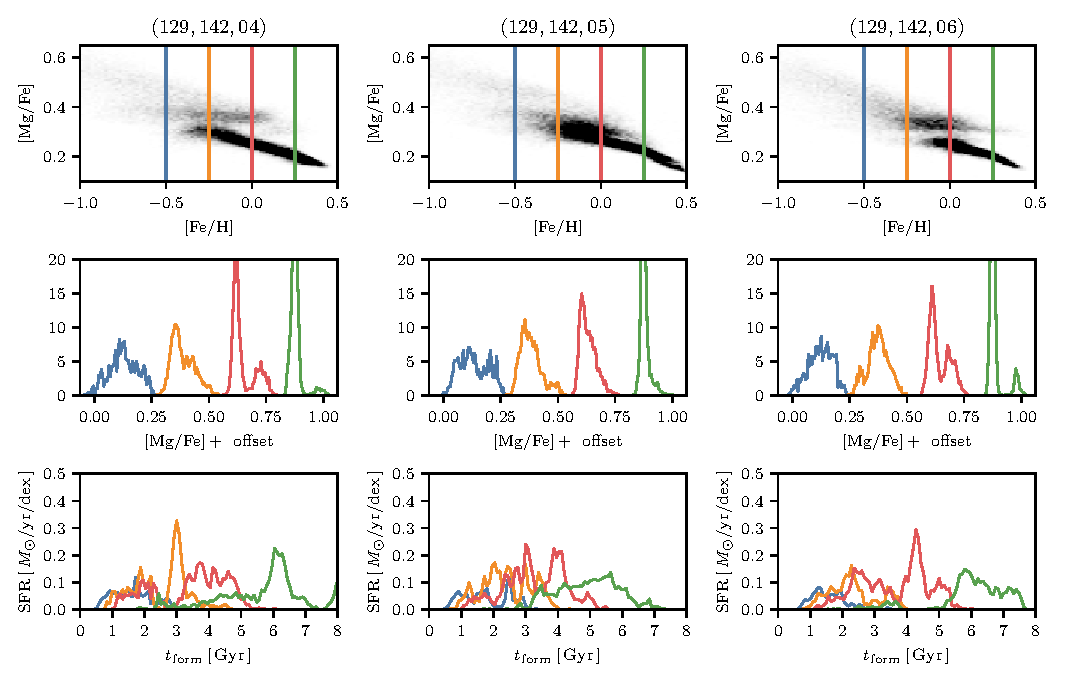
\includegraphics[width=\textwidth]{ch3/allmerge5.pdf}
  \caption{A continuation of Figure~\ref{fig:allmerge0}.}
  \label{fig:allmerge5}
\end{figure*}

\begin{figure*}
  \centering
  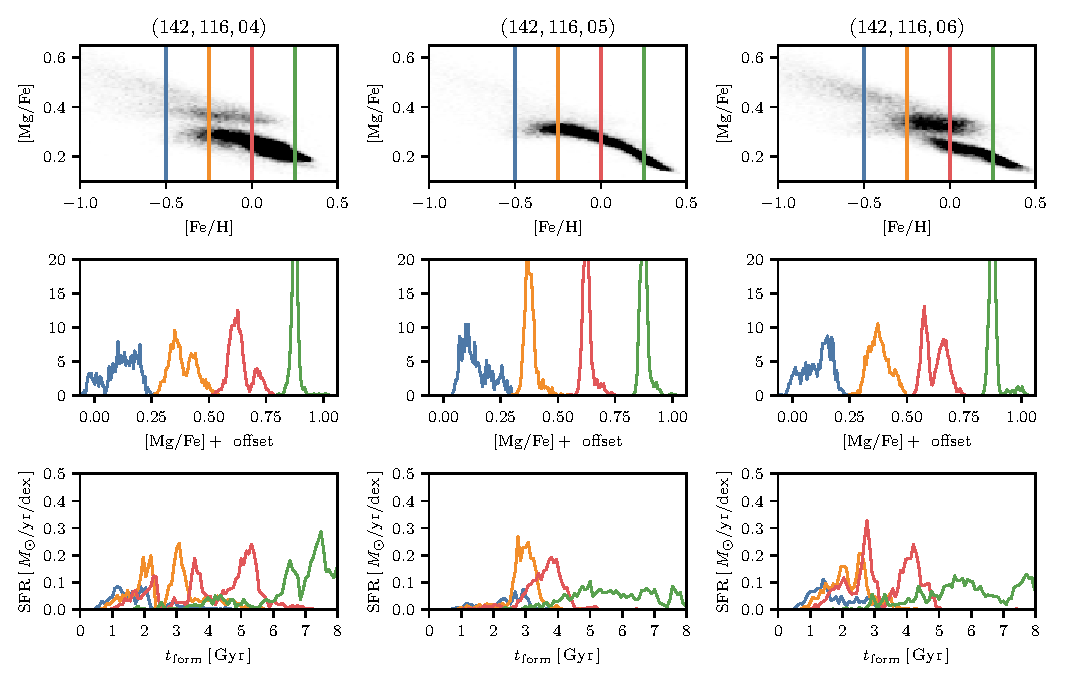
\includegraphics[width=\textwidth]{ch3/allmerge6.pdf}
  \caption{A continuation of Figure~\ref{fig:allmerge0}.}
  \label{fig:allmerge6}
\end{figure*}

\begin{figure*}
  \centering
  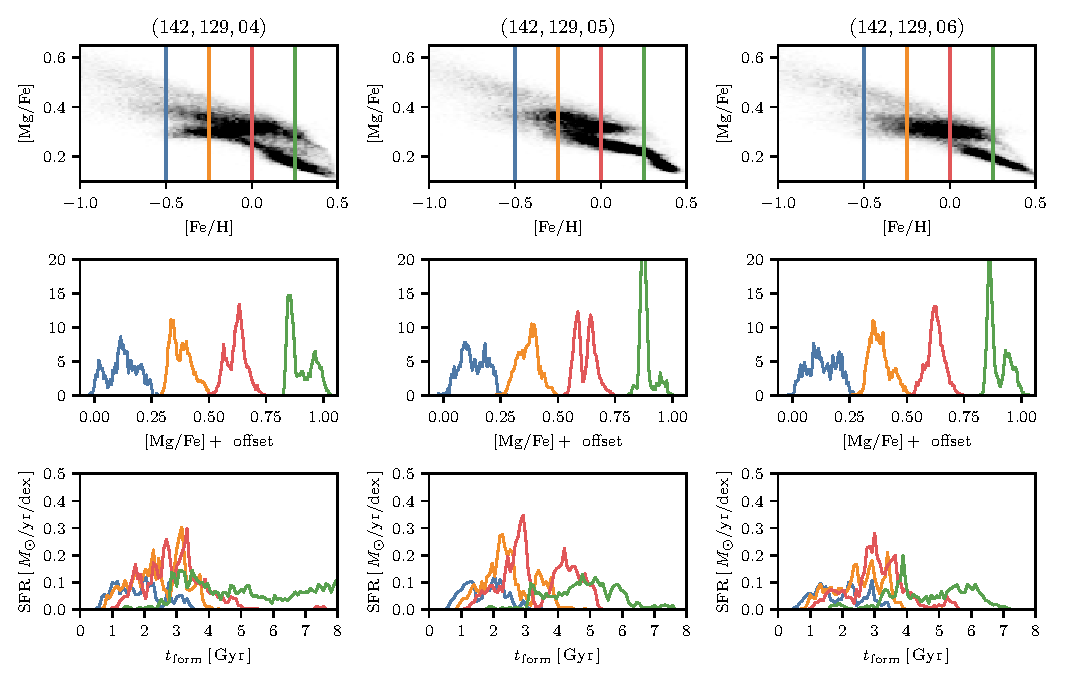
\includegraphics[width=\textwidth]{ch3/allmerge7.pdf}
  \caption{A continuation of Figure~\ref{fig:allmerge0}.}
  \label{fig:allmerge7}
\end{figure*}

\begin{figure*}
  \centering
  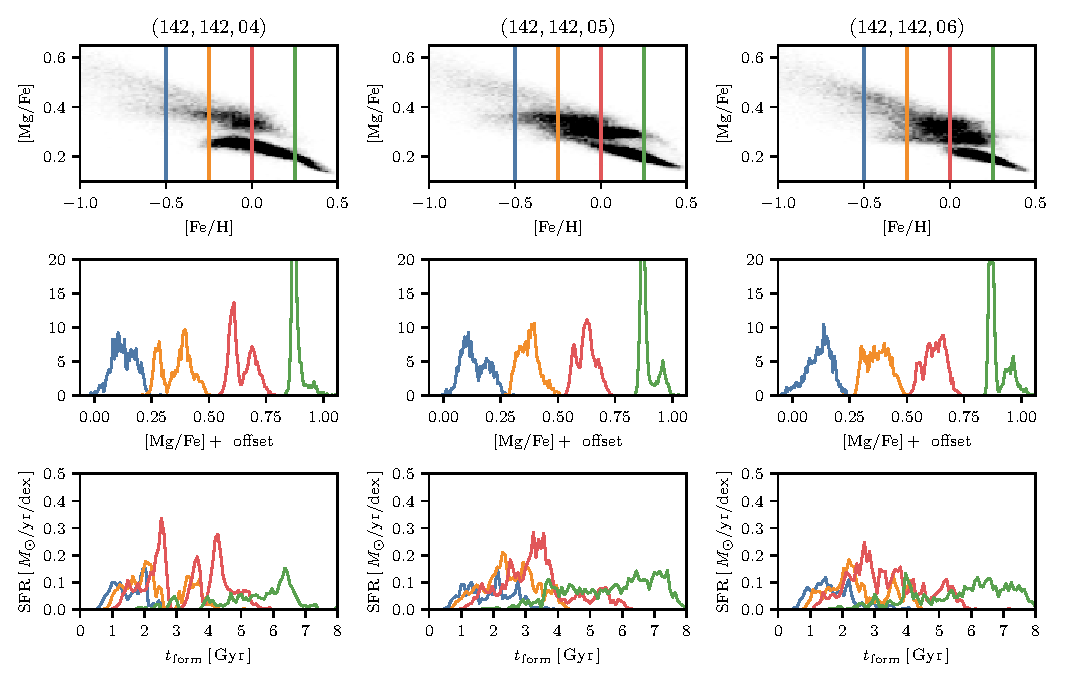
\includegraphics[width=\textwidth]{ch3/allmerge8.pdf}
  \caption{A continuation of Figure~\ref{fig:allmerge0}.}
  \label{fig:allmerge8}
\end{figure*}

\chapter{Appendix to Chapter~\ref{ch:Mgdec}}\label{ch:app_Mgdec}
\section{Observational Errors}\label{ch4:app:obs_err}
In Figure~\ref{fig:alpha}, we assumed observational errors of $12.5\%$ in age and $0.015\,\dex$ in \MgFe{}. In Figure~\ref{fig:obs_err}, we plot the quoted observational errors of the APOKASC-3 (left) and ASPCAP (right) datasets, showing both \FeH{} and \MgFe{} (blue and orange, respectively). We show our $12.5\%$ age error as a black line in the left panel. We take the age error to be the maximum of the upper and lower errors from \citet{2018ApJS..239...32P}. In the right panel, we show blue and orange vertical lines at $0.01$ and $0.015\,\dex$ for \FeH{} and \MgFe{}, respectively. These are approximately the 99th percentiles of each error distribution. As a dashed line we show our $25\%$ age error cut for stars plotted in Figure~\ref{fig:obs_err}. Our assumed errors are generally consistent with the errors quoted in the dataset, with a conservative estimate for the abundance errors.

\begin{figure*}
  \centering
  \includegraphics[width=\columnwidth]{ch4/obs_error.pdf}
  \caption{The observational errors of astroseismic ages from APOKASC-3 (left) and abundances from ASPCAP DR17 (right). We show, on the left, a line indicating a $12.5\%$ error in observed age and on the right a vertical line indicating a $0.01$ and $0.015\,\dex$ error in \FeH{} and \MgFe{}, respectively. On the left, a dashed line indicates the $25\%$ error cut used for inclusion in Figure~\ref{fig:alpha}.}
  \label{fig:obs_err}
\end{figure*}

\section{Random Selection of Subhalos}\label{ch4:app:rand_fig1}
In Figure~\ref{fig:app0}, we show the abundance plane of our fiducial galaxy at $z=0$. This reproduces the middle column of Figure~\ref{fig:fig1}. We also show the effect of our $\alpha$-enhancement procedure on this distribution when applied, from left to right, at redshifts of $1$, $1.5$, and $2$. (The $z=1.5$ column reproduces the right column of Figure~\ref{fig:fig1}). Qualitatively, the time at which the $\alpha$-enhancement is applied does not alter whether substructure arises in this plane. However, when it is applied at lower $z$, the peaks between modes do appear to be slightly further apart.

We show the same figure but with an additional random selection of 16 galaxies in the Milky Way-progenitor mass sample as a figure set (17 images), which is available in the online journal. Six additional galaxies (143882, 167392, 348901, 425719, 439099, and 465255) display bimodalities, though none as prominent as the main galaxy studied in this work. Some substructure is present in many galaxies. In general, the $\alpha$-enhancement increases the strength of substructure in the abundance planes. The fact that bimodalities like in the main galaxy studied in this work do not universally appear in $\alpha$-enhanced galaxies indicates that the $\alpha$-enhancement is not solely responsible for the bimodality.

The timing of the $\alpha$-enhancement does not have a major effect on our fiducial galaxy (Figure~\ref{fig:app0}). However, for some (e.g., the green $\FeH=-0.25$ bin in 439099), structure arises only when the $\alpha$-enhancement is applied at sufficiently low redshift. We interpret this as the presence of some substructure inducing activity between $z=1$ and 2.

\begin{figure*}
  \centering
  \includegraphics[width=\textwidth]{ch4/app_392276.pdf}
  \caption{Abundance plane of the fiducial galaxy at $z=0$ and the effects of $\alpha$-enhancement applied at different redshifts. The leftmost panel shows the fiducial galaxy without enhancement, reproducing the middle column of Figure~\ref{fig:fig1}. The subsequent panels from left to right show the results of applying $\alpha$-enhancement at redshifts of 1, 1.5, and 2, respectively. The $z=1.5$ column reproduces the right column of Figure~\ref{fig:fig1}. The presence of substructure in the abundance plane is consistent across different application times of $\alpha$-enhancement, though applying it at lower redshifts appears to slightly increase the separation between modal peaks. This figure is part of a set of 17 images available in the online journal, showing similar plots for 16 additional galaxies from our Milky Way-progenitor mass sample. The varied responses to $\alpha$-enhancement across the sample, with only six additional galaxies (143882, 167392, 348901, 425719, 439099, and 465255) displaying bimodalities, suggest that while $\alpha$-enhancement generally increases substructure, it is not solely responsible for creating bimodalities in abundance planes.}
  \label{fig:app0}
\end{figure*}

\begin{figure*}
  \centering
  \includegraphics[width=\textwidth]{ch4/app_2.pdf}
  \caption{The same as Figure~\ref{fig:app0}, but for a random galaxy from our initial catalog.}
  \label{fig:app1}
\end{figure*}

\begin{figure*}
  \centering
  \includegraphics[width=\textwidth]{ch4/app_10.pdf}
  \caption{The same as Figure~\ref{fig:app0}, but for a random galaxy from our initial catalog.}
  \label{fig:app2}
\end{figure*}

\begin{figure*}
  \centering
  \includegraphics[width=\textwidth]{ch4/app_143882.pdf}
  \caption{The same as Figure~\ref{fig:app0}, but for a random galaxy from our initial catalog.}
  \label{fig:app3}
\end{figure*}

\begin{figure*}
  \centering
  \includegraphics[width=\textwidth]{ch4/app_167392.pdf}
  \caption{The same as Figure~\ref{fig:app0}, but for a random galaxy from our initial catalog.}
  \label{fig:app4}
\end{figure*}

\begin{figure*}
  \centering
  \includegraphics[width=\textwidth]{ch4/app_289388.pdf}
  \caption{The same as Figure~\ref{fig:app0}, but for a random galaxy from our initial catalog.}
  \label{fig:app5}
\end{figure*}

\begin{figure*}
  \centering
  \includegraphics[width=\textwidth]{ch4/app_300903.pdf}
  \caption{The same as Figure~\ref{fig:app0}, but for a random galaxy from our initial catalog.}
  \label{fig:app6}
\end{figure*}

\begin{figure*}
  \centering
  \includegraphics[width=\textwidth]{ch4/app_348901.pdf}
  \caption{The same as Figure~\ref{fig:app0}, but for a random galaxy from our initial catalog.}
  \label{fig:app7}
\end{figure*}

\begin{figure*}
  \centering
  \includegraphics[width=\textwidth]{ch4/app_398784.pdf}
  \caption{The same as Figure~\ref{fig:app0}, but for a random galaxy from our initial catalog.}
  \label{fig:app8}
\end{figure*}

\begin{figure*}
  \centering
  \includegraphics[width=\textwidth]{ch4/app_404818.pdf}
  \caption{The same as Figure~\ref{fig:app0}, but for a random galaxy from our initial catalog.}
  \label{fig:app9}
\end{figure*}

\begin{figure*}
  \centering
  \includegraphics[width=\textwidth]{ch4/app_425719.pdf}
  \caption{The same as Figure~\ref{fig:app0}, but for a random galaxy from our initial catalog.}
  \label{fig:app10}
\end{figure*}

\begin{figure*}
  \centering
  \includegraphics[width=\textwidth]{ch4/app_439099.pdf}
  \caption{The same as Figure~\ref{fig:app0}, but for a random galaxy from our initial catalog.}
  \label{fig:app11}
\end{figure*}

\begin{figure*}
  \centering
  \includegraphics[width=\textwidth]{ch4/app_465255.pdf}
  \caption{The same as Figure~\ref{fig:app0}, but for a random galaxy from our initial catalog.}
  \label{fig:app12}
\end{figure*}

\begin{figure*}
  \centering
  \includegraphics[width=\textwidth]{ch4/app_494709.pdf}
  \caption{The same as Figure~\ref{fig:app0}, but for a random galaxy from our initial catalog.}
  \label{fig:app13}
\end{figure*}

\begin{figure*}
  \centering
  \includegraphics[width=\textwidth]{ch4/app_510273.pdf}
  \caption{The same as Figure~\ref{fig:app0}, but for a random galaxy from our initial catalog.}
  \label{fig:app14}
\end{figure*}

\begin{figure*}
  \centering
  \includegraphics[width=\textwidth]{ch4/app_547293.pdf}
  \caption{The same as Figure~\ref{fig:app0}, but for a random galaxy from our initial catalog.}
  \label{fig:app15}
\end{figure*}

\begin{figure*}
  \centering
  \includegraphics[width=\textwidth]{ch4/app_576516.pdf}
  \caption{The same as Figure~\ref{fig:app0}, but for a random galaxy from our initial catalog.}
  \label{fig:app16}
\end{figure*}

\chapter{The Emergence of Human Consciousness}
\begin{adjustwidth}{.8cm}{0cm}
\textit{Three things can not hide for long: the Moon, the Sun and the Truth.}

\hspace{9cm} -- Siddhartha Gautama
\end{adjustwidth}

\noindent
We now broaden our interests considerably. One of the great mysteries of our time is that the sun and moon have approximately the same apparent diameter on the sky, an apparent coincidence. However, because the moon is receding from the Earth, a more precise statement is that the coincidence is between the timing of the emergence of human consciousness at a time when the sun and moon have the same apparent diameter.

A natural outcome of the similar size of the sun and moon is the presence of total solar eclipses. However, because they have such similar sizes on the sky, total solar eclipses are quite rare, occurring about once every 375 years for a given spot on Earth \citep[varying somewhat with latitude][]{2002mmam.book.....M}. Given the current recession rate of the moon of $\sim3.8\,\textrm{cm}/\textrm{yr}$, the semi-major axis of the moon would have been $\sim0.02\,\%$ smaller when \textit{Homo erectus} emerged $\sim2\,\Myr$ ago, implying a very minor change to the overall occurrence of total solar eclipses. Assuming a generational turnover of $20\,\textrm{yr}$ \citep{homoerectus_lifespan}, this means that \textit{H. erectus} on average witnessed a solar eclipse about once every 18 generations.\footnote{This estimate is agnostic to whether they had a nomadic or sedentary lifestyle, since any movement patterns would be uncorrelated with impending eclipses. Note also that a given lineage from $2\,\Myr$ ago to the present would encounter about 5k eclipses, assuming 20~years between each generation.} This begs the question of how they would interpret such an event, and if it may lead to any appreciable effect on their long-term evolutionary outcome.

The answer is likely not, but it is even more likely that no one is still reading, so we can continue. Does witnessing totality confer any advantage for the emergence of consciousness? Because there is no genetic bias towards who would witness an eclipse, the effect must be of second-order. As an illustrative example, the attempt of a small child to understand an eclipse might push their brain to develop a slightly higher mental capacity. Some children will be able to develop this capacity at a higher rate than others because of random genetic mutations, and it is those children who are conferred an evolutionary advantage. The fact these events happen on generational timescales only enforce their power.

To be clear, this proposition is by no means a direct cause and effect argument. It is clearly not the case that consciousness emerged during the first-ever solar eclipse. However, the fact that the sun and moon have the same apparent size on the sky, and that solar eclipses happen regularly but with an occurrence that makes them a powerful and mysterious event, may have made the arising of consciousness go from being a $20\sigma$ event to an $18\sigma$ event.

\end{appendices}


\end{document}
